\documentclass[fleqn]{NotesClass}

%% Packages
\usepackage{csquotes}
\usepackage{cancel}
\usepackage[greek, UKenglish]{babel}
\usepackage{mathtools}
\usepackage{subcaption}
\usepackage[version=4]{mhchem}

% Tikz stuff
\usepackage{tikz}
\tikzset{>=latex}
% £xternal
\usetikzlibrary{external}
\tikzexternalize[prefix=tikz-external/]
%\tikzexternaldisable
% Other libraries
\usetikzlibrary{angles}
\usetikzlibrary{quotes}
\usetikzlibrary{3d}
\usetikzlibrary{calc}
\usetikzlibrary{decorations.pathmorphing}

% References, should be last things loaded
\usepackage{hyperref}  % Should be loaded second last (cleveref last)
\colorlet{hyperrefcolor}{blue!60!black}
\hypersetup{colorlinks=true, linkcolor=hyperrefcolor, urlcolor=hyperrefcolor}
\usepackage[
capitalize,
nameinlink,
noabbrev
]{cleveref} % Should be loaded last

% My packages
\usepackage{NotesBoxes}
\usepackage{NotesMaths}


% Title page info
\title{Lagrangian Dynamics}
\author{Willoughby Seago}
\date{September 20, 2021}
% \subtitle{}
% \subsubtitle{}

% Highlight colour
\definecolor{highlight}{HTML}{255029}
\definecolor{complementaryteal}{HTML}{254C50}
\definecolor{complementarypurple}{HTML}{50254C}
\definecolor{complementaryred}{HTML}{502925}
%% Commands
% Text


% Maths
\newcommand*{\e}{\mathrm{e}}
\newcommand*{\vedot}[1]{\dot{\vv{e}}_{\vv{#1}}}
\newcommand*{\eff}{\mathrm{eff}}
\newcommand*{\order}{\mathcal{O}}
\newcommand*{\ext}{\mathrm{ext}}
\newcommand*{\constraint}{\mathrm{constraint}}
\newcommand*{\other}{\mathrm{other}}
\newcommand*{\nodependence}[1]{\textcolor{gray}{\cancel{#1}}}
\newcommand*{\lagrangian}{\mathcal{L}}
\newcommand*{\hamiltonian}{\mathcal{H}}
\DeclarePairedDelimiterX{\poissonbracket}[2]{\{}{\}}{#1, #2}
\DeclarePairedDelimiterX{\commutator}[2]{[}{]}{#1, #2}
\newcommand*{\DL}[1]{\mathcal{D}#1}
\newcommand*{\ident}{I}
\newcommand*{\trans}{\top}

% Include
\includeonly{parts/appendix-odes}

\begin{document}
    \frontmatter
    \titlepage
    \innertitlepage{tikz-external/effective-central-potential.pdf} 
    \tableofcontents
    \mainmatter
    \chapter{Introduction}
    The Lagrangian formalism of classical mechanics was pioneered by Joseph-Louis Lagrange.
    It is an alternative to Newton's formulation of classical mechanics.
    In many ways it is more powerful than Newton's formulation.
    For example, the Lagrangian formalism can easily include constraints on the system and is readily adapted to apply to electromagnetism, quantum mechanics, and relativistic systems.
    A task which is either impossible or incredibly difficult for the Newtonian formalism.
    Another benefit is that the Lagrangian formalism is built upon scalar quantities, which are often easier to work with than vectors.
    
    \part{Preparing for the Lagrangian Formalism}
    \chapter{Newton's Laws and Conservation Laws}
    \section{Newton's Laws}
    Newtonian mechanics is based on Newton's laws, a set of three laws that combined allow us to describe mechanics at everyday scales, that is when things are: not too fast (so no need for special relativity), not too massive (so no need for general relativity), and not too small (so no need for quantum mechanics).
    
    Before we can state Newton's laws we will need a few bits of notation and basic definitions.
    For now we consider point like particles and measure their position relative to some origin, \(O\).
    \begin{ntn}{Basic Quantities}{}
        \begin{itemize}
            \item \(\vv{r}\) denotes the position vector.
            \item \(\vv{v}\) denotes the velocity vector.
            \item \(\vv{a}\) denotes the acceleration vector.
            \item \(\vv{p}\) denotes the linear momentum vector.
            \item Given some differentiable quantity, \(f\), we denote by \(\dot{f}\) the total time derivative, \(\diff{f}/{t}\), and by \(\ddot{f}\) the second total time derivative, \(\diff[2]{f}/{t}\).
            We should not have use of higher time derivatives but if we do then the it should be clear how this dot notation generalises.
        \end{itemize}
    \end{ntn}
    
    \begin{dfn}{Basic Quantities}{}
        \begin{itemize}
            \item The \defineindex{velocity} is defined by \(\vv{v} \coloneqq \dot{\vv{r}}\).
            \item The \defineindex{acceleration} is defined by \(\vv{a} = \dot{\vv{v}} = \ddot{\vv{r}}\).
            \item The \define{momentum}\index{momentum!linear} is defined by \(\vv{p} = m\vv{v}\).
        \end{itemize}
    \end{dfn}
    
    We can now state Newton's laws.
    \paragraph{N1} \defineindex{Newton's first law} (N1)\glossary[acronym]{N1}{Newton's first law} states that in the absence of forces \(\vv{v}\) is constant.
    \paragraph{N2} \defineindex{Newton's second law} (N2)\glossary[acronym]{N2}{Newton's second law} states that in the presence of a force, \(\vv{F}\), the rate of change of linear momentum is \(\dot{\vv{p}} = \vv{F}\).
    A special case of this is when the mass is constant, which we will assume unless stated otherwise, in which case we recover the famous
    \begin{equation}
        \dot{\vv{p}} = m\dot{\vv{v}} = m\vv{a} = \vv{F}.
    \end{equation}
    In Newtonian mechanics we start most problems by assuming that the force, \(\vv{F}\) is either known or can be easily found.
    We then solve N2 for the equations of motion.
    \paragraph{N3} \defineindex{Newton's third law} (N3)\glossary[acronym]{N3}{Newton's third law} comes in two forms, a weak form and a strong form.
    In both we consider the force \(\vv{F_{ab}}\), which is the force on particle \(a\) due to particle \(b\).
    The weak form states that \(\vv{F_{ab}} = -\vv{F_{ba}}\).
    The strong form states that as well as this \(\vv{F_{ab}}\) is directed along \(\vv{r_{ab}} = \vv{r_a} - \vv{r_b}\) where \(\vv{r_a}\) is the position of \(a\) and \(\vv{r_b}\) the position of \(b\).
    
    \subsection{Caveats}
    Newton's laws all come with caveats.
    Obviously, due to the need for quantum mechanics and relativity, Newton's laws aren't always valid.
    So, we need to be careful about when we apply them.
    
    N1 and N2 are only valid in non-accelerating frames, that is when there are no external forces.
    We call these \define{inertial frames}\index{inertial frame}.
    We typically assume frames are inertial unless stated otherwise.
    Apart from linearly accelerating frames it should be noted that rotating frames aren't inertial, even for a constant rotation speed.
    This, as well as the movement around the sun, and movement of the solar system, and movement of the solar system, and the movement of the galaxy and, \dots, means that the Earth is \emph{not} an inertial frame.
    However, it is a sufficiently good approximation of an inertial frame for most of our everyday requirements.
    There are a few cases, such as Foucault's pendulum, where the rotation of the Earth has a non-negligible effect.
    
    Both forms of N3 only hold for types of force.
    For example, since the force from a magnetic field is orthogonal to the velocity, means that in general the strong form of N3 doesn't hold for charged particles.
    
    \section{Conservation Laws}
    Conservation laws are \emph{incredibly} important in physics.
    One advantage of the Lagrangian formalism is how easy it is to find conservation laws with it.
    However, for now we restrict our selves to deriving the most important conservation laws from the Newtonian formalism.
    
    \subsection{Conservation of Linear Momentum}
    Suppose there is no force, so \(\vv{F} = \vv{0}\).
    It immediately follows from N2 that \(\dot{\vv{p}} = \vv{F} = \vv{0}\) and hence \(\vv{p}\) is constant.
    We say that in the absence of external forces linear momentum is conserved.
    A consequence of this is that if \(m\) is a constant then \(\vv{a} = \vv{0}\) and so the particle travels at a constant velocity.
    
    \subsection{Conservation of Angular Momentum}
    \begin{dfn}{Angular Momentum and Torque}{}
        For a particle at position \(\vv{r}\) and linear momentum \(\vv{p}\) we define its \define{angular momentum}\index{momentum!angular} with respect to the origin to be
        \begin{equation}
            \vv{L} \coloneqq r\times \vv{p}.
        \end{equation}
        If a force, \(\vv{F}\), is applied to the particle then we define the \defineindex{torque}, also known as the \defineindex{moment of force} about the origin to be
        \begin{equation}
            \vv{G} \coloneqq \vv{r} \times \vv{F}.
        \end{equation}
    \end{dfn}
    Note that since they are defined via cross products both \(\vv{L}\) and \(\vv{G}\) are axial vectors (aka pseudovectors), meaning that if we change between a left and right handed coordinate system then these vectors change sign.
    
    Applying N2 to the definition of torque we have
    \begin{equation}
        \vv{G} = \vv{r}\times\vv{F} = \vv{r}\times\dot{\vv{p}} = \diff*{(\vv{r}\times\vv{p})}{t} - \dot{\vv{r}}\times\vv{p}
    \end{equation}
    where in the last step we have used the chain rule:
    \begin{equation}
        \diff*{(\vv{r}\times\vv{p})}{t} = \vv{r}\times\dot{\vv{p}} + \dot{\vv{r}}\times\vv{p} \implies \vv{r}\times\dot{\vv{p}} = \diff*{(\vv{r}\times\vv{p})}{t} - \dot{\vv{r}}\times\vv{p}.
    \end{equation}
    We now look at this last term, \(\dot{\vv{r}}\times\vv{p}\), in more detail.
    Noticing that \(\dot{\vv{r}} =\vv{v}\) and \(\vv{p} = m\vv{v}\) we see that this term is zero, since the cross product of any two collinear vectors is zero.
    Hence,
    \begin{equation}
        \vv{G} = \diff*{(\vv{r}\times\vv{p})}{t} = \dot{\vv{L}}
    \end{equation}
    where we have used the definition of angular momentum, \(\vv{L} = \vv{r}\times\vv{p}\).
    From this we see that if \(\vv{G} = \vv{0}\) then \(\dot{\vv{L}} = \vv{0}\) and hence \(\vv{L}\) is constant.
    We say that in the absence of external torques angular momentum is conserved.
    
    \subsection{Conservation of Energy}
    \begin{dfn}{Work Done}{}
        The \defineindex{work done} to move a particle along a path, \(\Gamma\), requiring force \(\vv{F}\) is defined as
        \begin{equation}
            W\coloneqq \int_\Gamma \vv{F}\cdot\dl{\vv{r}}.
        \end{equation}
    \end{dfn}
    
    Consider the work done to move a particle from \(A\) to \(B\) along some path, which we parametrise as a function of \(t\) (which may or may not be time) such that when \(t = t_A\) the particle is at \(A\) and when \(t = t_B\) the particle is at \(B\).
    We will assume a constant mass but the following result holds for a variable mass, the derivation is just more involved.
    \begin{align}
        W_{AB} &= \int_A^B \vv{F}\cdot\dl{\vv{r}}\\
        &= \int_{t_A}^{t_B} \vv{F} \cdot\diff{\vv{r}}{t}\dd{t}\\
        &= \int_{t_A}^{t_B} \dot{\vv{p}}\cdot\vv{v}\dd{t}\\
        &= \int_{t_A}^{t_B} m\dot{\vv{v}}\cdot\vv{v}\dd{t}\\
        &= \frac{m}{2}\int_{t_A}^{t_B} v^2 \dd{t}\\
        &= \frac{m}{2}[v^2]_{t_A}^{t_B}\\
        &= \frac{1}{2}m[v(t_B)]^2 - \frac{1}{2}[v(t_A)]^2\\
        &= T_{B} - T_{A}\label{eqn:W=Tb-Ta}
    \end{align}
    where \(T\coloneqq \frac{1}{2}mv^2\) defines the \defineindex{kinetic energy} in Newtonian mechanics.
    Note that about halfway through the calculation we used
    \begin{equation}
        \diff*{(\vv{v}\cdot\vv{v})}{t} = \vv{v}\cdot\dot{\vv{v}} + \dot{\vv{v}}\cdot\vv{v} = 2\dot{\vv{v}}\cdot\vv{v} \implies \dot{\vv{v}}\cdot\vv{v} = \frac{1}{2}\diff*{(\vv{v}\cdot\vv{v})}{t}.
    \end{equation}
    We can see from this that the work done on a particle is equal to the change in kinetic energy of the particle.
    
    \begin{dfn}{Conservative Force}{}
        The following are equivalent:
        \begin{itemize}
            \item The force \(\vv{F}\) is \define{conservative}\index{conservative force}.
            \item The work done to move a particle from \(A\) to \(B\) is independent of the path taken, that is
            \begin{equation}
                \int_\Gamma \vv{F}\cdot\dl{\vv{r}} = \int_\gamma \vv{F}\cdot\dl{\vv{r}}
            \end{equation}
            where \(\Gamma\) and \(\gamma\) are two paths from \(A\) to \(B\).
            \item The following holds
            \begin{equation}
                \oint \vv{F}\cdot\dl{\vv{r}} = 0
            \end{equation}
            where \(\oint\) denotes an integral over a closed path, that is a path that starts and ends at the same point.
            \item There exists a scalar function, \(V\), such that
            \begin{equation}
                \vv{F} = -\grad V.
            \end{equation}
            \item The following holds
            \begin{equation}
                \curl\vv{F} = \vv{0}.
            \end{equation}
        \end{itemize}
    \end{dfn}
    
    Suppose \(\vv{F}\) is a conservative force.
    Then we can write \(\vv{F} = -\grad V\) for some scalar function \(V\). The negative sign here is just a convention so that we can minimise the potential, instead of maximising, which better aligns with our intuition and the original definition of potentials before this more general notion.
    We can use this to redo the calculation above:
    \begin{align}
        W_{AB} &= \int_{A}^{B}\vv{F}\cdot\dl{\vv{r}}\\
        &= -\int_A^B \grad V \cdot\dl{\vv{r}}\\
        &= -\int_A^B\dd{V}\\
        &= V_B - V_A\label{eqn:W=Vb-Va}
    \end{align}
    where \(V_A\) and \(V_B\) are the value of the potential at \(A\) and \(B\) respectively.
    Note here that we used
    \begin{equation}
        \int\grad V\cdot\dl{\vv{r}} = \int\dd{V}
    \end{equation}
    which is the three dimensional analogue of
    \begin{equation}
        \int \diff{f}{x}\dd{x} = \int\dd{f}
    \end{equation}
    
    Combining \cref{eqn:W=Tb-Ta,eqn:W=Vb-Va} we get
    \begin{equation}
        T_A + V_A = T_B + V_B
    \end{equation}
    we define \(E \coloneqq T + V\) to be the \defineindex{total energy} and since this equation holds for any two points \(A\) and \(B\) this shows that, for a conservative force, the total energy is conserved.
    Since most, but not all, forces we meet in classical mechanics are conservative this is a very useful property.
    
    \chapter{Orbits}
    In this section we apply Newton's laws and conservation laws to one of the systems that motivated their development: orbiting planets.
    More generally we will consider some particle moving in a central force field described by a \defineindex{central potential} \(V(\vv{r}) = V(r)\).
    Our goal is to find an equation for the radial velocity of an orbiting particle.
    
    \section{Central Force}
    Recall that a \defineindex{central force} is one which depends only on the magnitude, \(r\), of the position vector, \(\vv{r}\) and acts along the line to the origin: \(\vv{F}(\vv{r}) = F(r)\vh{r} = -\grad V(r)\).
    Here \(\vh{r} = \vv{r}/r\) is a unit vector in the direction of the position vector.
    
    \subsection{Momenta}
    Assuming that \(\vv{F} \ne \vv{0}\) linear momentum will not be conserved.
    We can easily calculate the torque:
    \begin{equation}
        \vv{G} = \vv{r}\times\vv{F} = \vv{r}\times\vh{r}F = \vv{0}
    \end{equation}
    since the cross product of two collinear vectors is identically zero.
    Since there is no torque the angular momentum, \(\vv{L}\), is conserved.
    In particular the magnitude of the angular momentum, \(L\), is a constant.
    We have that
    \begin{equation}
        \vv{r}\cdot\vv{L} = \vv{r}\cdot(\vv{r}\times\vv{p}) = 0
    \end{equation}
    since \(\vv{r}\times\vv{p}\) is perpendicular to \(\vv{r}\).
    What we have here is of the form \(\vv{r}\) dotted with a constant vector equals a constant.
    This defines a plane perpendicular to the constant vector.
    The physical interpretation of this is that the particle is constrained to motion in the plane with normal \(\vv{L}\) containing the origin.
    
    \subsection{Coordinates}
    Since the particle is constrained to a plane we work in cylindrical polar coordinates, \((r, \varphi, z)\), with the \(\vh{z}\)-axis perpendicular to the plane of motion.
    In these coordinates
    \begin{align}
        x &= r\cos\varphi,\\
        y &= r\sin\varphi,\\
        z &= z,
    \end{align}
    where \(r = \abs{\vv{r}} = \sqrt{x^2 + y^2}\).
    In the plane of motion \(z = 0\).
    
    We define two orthonormal basis vectors, \(\ve{r}\) and \(\ve{\varphi}\), which are parallel and perpendicular, respectively, to the position vector, \(\vv{r}\).
    At the point \((r, \varphi, z)\) these vectors are given in terms of the Cartesian unit vectors, \(\ve{x}\), \(\ve{y}\), and \(\ve{z}\), by
    \begin{align}
        \ve{r} &\coloneqq \hphantom{-}\cos\varphi\ve{x} + \sin\varphi\ve{y}\label{eqn:e_r definition}\\
        \ve{\varphi} &\coloneqq -\sin\varphi\ve{x} + \sin\varphi\ve{y}.
    \end{align}
    The position vector is then
    \begin{equation}
        \vv{r} = x\ve{x} + y\ve{y} = r\ve{r}.
    \end{equation}
    
    \subsection{Velocity}
    The velocity of the particle can be found by differentiating the position vector with respect to time:
    \begin{align}
        \vv{v} &= \dot{\vv{r}}\\
        &= \diff*{(r\ve{r})}{t}\\
        &= \dot{r}\ve{r} + r\vedot{r}
    \end{align}
    Notice that, unlike Cartesian unit vectors, the cylindrical unit vectors are time dependent\footnote{rather, they're position dependent and the position is time dependent} and so we have a second term involving the derivative of the unit vector.
    We can easily work out what this is by differentiating \cref{eqn:e_r definition}:
    \begin{align}
        \vedot{r} &= \diff*{(\cos\varphi\ve{x} + \sin\varphi\ve{y})}{t}\\
        &= -\dot{\varphi}\sin\varphi\ve{x} + \dot{\varphi}\cos\varphi\ve{y}\\
        &= \dot{\varphi}\ve{\varphi}.
    \end{align}
    Substituting this into the velocity we have
    \begin{equation}
        \dot{\vv{r}} = \dot{r}\ve{r} + r\dot{\varphi}\ve{\varphi}.
    \end{equation}
    We can see from this that the radial velocity is \(v_r = \dot{r}\), and the tangential component of the velocity is \(v_\varphi = r\dot{\varphi}\).
    
    \textcolor{highlight}{Be careful}: \(\dot{r} = v_r\) is not the same as \(\abs{\dot{\vv{r}}} = v\) here, for example, if motion is in a circle then \(\dot{r} = 0\) but \(\dot{\vv{r}} \ne \ve{0}\).
    
    \subsection{Using Conservation Laws}
    We can calculate the angular momentum now:
    \begin{align}
        \vv{L} &= \vv{r}\times\vv{p}\\
        &= \vv{r}\times\dot{\vv{r}}m\\
        &= mr[\ve{r} \times (\dot{r}\ve{r} + r\dot{\varphi}\ve{\varphi})]\\
        &= \vv{0} + mr^2\dot{\varphi}\ve{r}\times\ve{\varphi}\\
        &= mr^2\dot{\varphi}\ve{z}.
    \end{align}
    Since the angular momentum is conserved we know that \(L = mr^2\dot{\varphi}\) is constant.
    Inverting this relationship we have \(\dot{\varphi} = L/(mr^2)\), which will be useful in a moment.
    
    The kinetic energy is easy to find once we have an expression for the velocity:
    \begin{align}
        T &= \frac{1}{2}mv^2\\
        &= \frac{1}{2}m\dot{\vv{r}}\cdot\dot{\vv{r}}\\
        &= \frac{1}{2}m(\dot{r}^2 + r^2\dot{\varphi}^2).
    \end{align}
    The total energy is then
    \begin{align}
        E &= T + V\\
        &= \frac{1}{2}m(\dot{r}^2 + r^2\dot{\varphi}^2) + V(r)\\
        &= \frac{1}{2}m\dot{r}^2 + \frac{L^2}{2mr^2} + V(r)\label{eqn:central force orbit energy}
    \end{align}
    where we have substituted for \(\dot{\varphi} = L/(mr^2)\).
    
    Notice that we can now write the total energy as
    \begin{equation}
        E = \frac{1}{2}m\dot{r}^2 + V_\eff(r)
    \end{equation}
    where
    \begin{equation}
        V_{\eff}(f) = \frac{L^2}{2mr^2} + V(r)
    \end{equation}
    is an \defineindex{effective potential}, that is the particle's motion in the radial direction (since we consider a \enquote{kinetic energy} \(m\dot{r}^2/2\), which considers motion only along the radial direction) behaves as if it is a particle constrained to one-dimensional motion in the potential \(V_\eff\).
    
    \subsection{Radial Velocity}
    Solving \cref{eqn:central force orbit energy} for \(\dot{r}\) we find
    \begin{equation}\label{eqn:central potential radial velocity}
        \dot{r} = \pm \left[ \frac{2}{m}\left( E - V(r) - \frac{L^2}{2mr^2} \right) \right]^{1/2}.
    \end{equation}
    Here \(E\) and \(L\) are conserved quantities fixed by the initial conditions.
    Since \(\dot{r}\) is real the quantity in square brackets on the right must be non-negative for all values of \(r\).
    From this we see that \(E \ge V_{\eff}(r)\) for all \(r\).
    
    \section{Inverse Square Law Force}
    We now restrict ourselves to the special case of
    \begin{equation}
        V(r) = -\frac{k}{r}.
    \end{equation}
    The force from this is
    \begin{equation}
        \vv{F}(\vv{r}) = -\frac{k}{r^2}\vh{r},
    \end{equation}
    which is an inverse square law.
    Hence this potential can describe gravitational attraction or electrostatic interactions.
    The effective potential in this case is
    \begin{equation}
        V_\eff(r) = \frac{L^2}{2mr^2} - \frac{k}{r}.
    \end{equation}
    This is plotted in \cref{fig:effective central potential}.
    
    \begin{figure}
        \tikzsetnextfilename{effective-central-potential}
        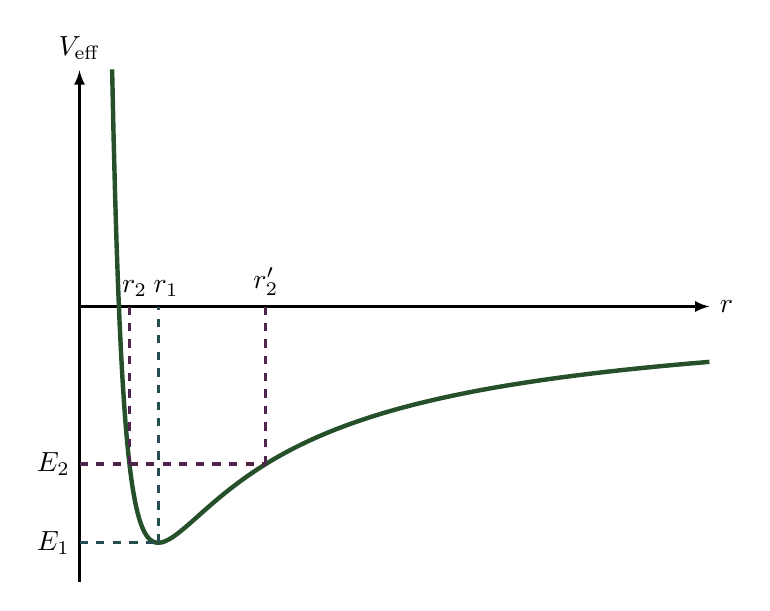
\begin{tikzpicture}
            \draw[->, thick] (0, -3.5) -- (0, 3) node[above] {\(V_\eff\)};
            \draw[->, thick] (0, 0) -- (8, 0) node[right] {\(r\)};
            \draw[domain=0.414:8, highlight, ultra thick, samples=400] plot (\x, {3*(\x^-2 - 2*\x^-1)});
            \draw[complementaryteal, dashed, very thick] (0, -3) -- (1, -3);
            \draw[complementaryteal, dashed, very thick] (1, -3) -- (1, 0);
            \node[above] at (1.1, 0) {\(r_1\)};
            \node[left] at (0, -3) {\(E_1\)};
            \draw[complementarypurple, dashed, very thick] (0, -2) -- (2.366, -2);
            \node[left] at (0, -2) {\(E_2\)};
            \draw[complementarypurple, dashed, very thick] (0.634, -2) -- (0.634, 0);
            \node[above] at (0.7, 0) {\(r_2\)};
            \draw[complementarypurple, dashed, very thick, text=black] (2.366, -2) -- (2.366, 0) node[above] {\(r_2'\)};
        \end{tikzpicture}
        \caption{The effective potential, \(V_{\eff}\).}
        \label{fig:effective central potential}
    \end{figure}
    
    Now consider the particular case where \(E = E_1 = \min V_{\eff}(r)\).
    In this case the particle is constrained to have \(r = r_1\) where \(r_1\) is the value that minimises \(V_\eff\).
    This corresponds to a stable circular orbit.
    
    If instead \(E = E_2 > E_1\) then the particle will be able to move in the radial direction.
    If \(E < 0\) then the particle will be constrained between two values \(r_2\) and \(r_2'\) which are such that \(V_{\eff}(r_2) = V_{\eff}(r_2') = E_2\).
    At \(r_2\) and \(r_2'\) we must have \(\dot{r} = 0\) since these are turning points.
    
    We can treat both of these two cases a bit more formally by considering the effective equation of motion for motion in the radial direction.
    We can find this using energy conservation since this implies \(\dot{E} = 0\):
    \begin{align}
        \diff{E}{t} &= \diff*{\left( \frac{1}{2}m\dot{r}^2 + V_{\eff}(r) \right)}{t}\\
        &= m\dot{r}\ddot{r} + \diff{V_{\eff}}{r}\dot{r}.
    \end{align}
    Since this holds for all \(\dot{r}\) we must have
    \begin{equation}
        m\ddot{r} = -\diff{V_{\eff}}{r}.\label{eqn:EoM central potential}
    \end{equation}
    
    \subsection{Circular Orbit}
    Suppose the particle is in a circular orbit with some fixed radius, \(r = r_1\).
    Then \(\dot{r} = 0\).
    This requires that \(E = V_{\eff}(r_1) = E_1\).
    Therefore a stable circular orbit is possible where the effective potential is a minima or maxima.
    
    Alternatively we know that \(r\) is constant so \(\dot{r}\) and \(\ddot{r}\) are zero meaning that \cref{eqn:EoM central potential} gives
    \begin{equation}
        0=\diff{V_{\eff}}{r}[r=r_1].
    \end{equation}
    
    \subsection{Perturbed Circular Orbit}
    Suppose we have a circular orbit of radius \(r_1\), and we perturb it by moving the particle a small amount, \(\varepsilon\), outwards.
    The radial velocity of the particle is simply
    \begin{equation}
        \dot{r} = \diff*{(r_1 + \varepsilon)}{t} = \dot{\varepsilon}
    \end{equation}

    For small \(\varepsilon\) we can Taylor expand the effective potential about \(r = r_1\):
    \begin{align}
        V_\eff(r) &= V_{\eff}(r_1 + \varepsilon)\\
        &= V_\eff(r_1) + \varepsilon\diff{V_{\eff}}{r}[r=r_1] + \frac{\varepsilon^2}{2}\diff[2]{V_{\eff}}{r}[r=r_1] + \order(\varepsilon^3)\\
        &= V_\eff(r_1) + \frac{k}{2}\varepsilon^2 + \order(\varepsilon^3).
    \end{align}
    Here we have used the fact that \(V_\eff'(r_1) = 0\) as this \(r_1\) is the location of the minimum.
    \(V_\eff(r_1)\) is just a constant and we have defined \(k = V_\eff''(r_1)\).
    Ignoring terms \(\order(\varepsilon^3)\) or smaller and dropping the constant \(V_{\eff}(r_1)\) term we have
    \begin{equation}
        E = \frac{1}{2}m\dot{\varepsilon}^2 + \frac{k}{2}\varepsilon^2.
    \end{equation}
    If \(k > 0\), i.e. \(r_1\) is a local minimum, then this is the energy of a harmonic oscillator of mass \(m\) and spring constant \(k\).
    The small perturbation then leads to the radial position oscillating with angular frequency \(\omega = \sqrt{k/m}\) about \(r_1\).
    
    If \(k < 0\), i.e. \(r_1\) is a local maximum, then the circular orbit is unstable and the perturbation will cause it to turn into some other kind of orbit.
    
    If \(k = 0\) then we can't ignore the \(\order(\varepsilon^3)\) terms in the Taylor expansion.
    
    \subsection{Zones of Motion}
    We showed in the previous example that motion was restricted to the zone \(r_{\mathrm{min}} \le r \le r_{\mathrm{max}}\) where the boundaries are the roots of \(V_{\eff}(r) = E\).
    
    This can be generalised by noticing that \cref{eqn:central potential radial velocity} is of the form
    \begin{equation}
        \dot{r} = \pm \sqrt{g(r)},
    \end{equation}
    in this case \(g(r) = 2(E - V_{\eff}(r))/m\).
    Since \(\dot{r}\) is strictly real this requires \(g(r)\) be positive.
    Therefore whatever happens (barring things like quantum tunnelling) the motion is restricted to th zone \(r_{\mathrm{min}} \le r \le r_{\mathrm{max}}\) where the boundaries are roots of \(g(r) = 0\) at which \(g\) crosses the axis.
    There may be multiple regions in which motion can occur but the system will not be able to move between them unaided.
    
    Analysing various zones of motion can be a powerful tool that allows us to find information about a system without needing to solve for the full trajectory, which is often a difficult task.
    To show that a coordinate is restricted to some zone first look for equations of the form \(\dot{r} = \pm\sqrt{g(r)}\).
   
    \chapter{Dynamics of a Particle System}
    In this section we will consider a system of \(N\) particles, each labelled by some index \(a = 1, \dotsc, N\).
    We suppose that the \(a\)th particle has constant mass \(m_a\) and its position is \(\vv{r_a}\).
    
    We start with Newton's second law for an individual particle:
    \begin{equation}
        m_a\ddot{\vv{r}}_{\vv{a}} = \vv{F_a}.
    \end{equation}
    The force \(\vv{F_a}\) is due to two different sources.
    First there is the external force, \(\vv{F_a^{\ext}}\), which may be, for example, gravity.
    There is also then the force due to interactions with all of the other particles, perhaps due to an electromagnetic interaction.
    We use \(\vv{F_{ab}}\) to denote the force on particle \(a\) due to particle \(b\).
    The total internal force on \(a\) is then given by summing over this interaction for all particles distinct from \(a\).
    The net force on the particle is then
    \begin{equation}
        \vv{F_a} = \vv{F_a^{\ext}} + \sum_{b \ne a} \vv{F_{ab}}.
    \end{equation}
    
    \section{Centre of Mass Motion}
    Summing Newton's law over all particles we get
    \begin{equation}
        \sum_{a} m_a\ddot{\vv{r}}_{\vv{a}} = \sum_a\vv{F_a} = \sum_a \vv{F_a^{\ext}} + \sum_a \sum_{b\ne a} \vv{F_{ab}}.
    \end{equation}
    Focussing on this last term with a double sum we see that it is possible to write it as a single sum over pairs of particles,
    \begin{equation}
        \sum_{a}\sum_{b\ne a} \vv{F_{ab}} = \sum_{\text{pairs}} (\vv{F_{ab}} + \vv{F_{ba}}).
    \end{equation}
    To see this consider the explicit example of three particles:
    \begin{align}
        \sum_{a=1}^{3}\sum_{\substack{b\in\{1, 2, 3\}\\b\ne a}} \vv{F_{ab}} &= \vv{F_{12}} + \vv{F_{13}} + \vv{F_{21}} + \vv{F_{23}} + \vv{F_{31}} + \vv{F_{32}}\\
        &= (\vv{F_{12} + \vv{F_{21}}}) + (\vv{F_{13}} + \vv{F_{31}}) + (\vv{F_{23}} + \vv{F_{32}}).
    \end{align}
    
    It follows, assuming the weak form of Newton's third law, that \(\vv{F_{ba}} = -\vv{F_{ab}}\) and hence
    \begin{equation}
        \sum_{a}\sum_{b\ne a} \vv{F_{ab}} = \sum_{\text{pairs}}(\vv{F_{ab}} + \vv{F_{ba}}) = \sum_{\text{pairs}} (\vv{F_{ab}} - \vv{F_{ab}}) = \vv{0}.
    \end{equation}
    So, all internal forces cancel pairwise.
    Hence
    \begin{equation}
        \sum_a m_a\ddot{\vv{r}}_{\vv{a}} = \sum_a \vv{F_{a^{\ext}}} \eqqcolon \vv{F^{\ext}}
    \end{equation}
    where we have defined \(\vv{F^{\ext}}\) to be the net external force on the system.
    Defining the total mass
    \begin{equation}
        M \coloneqq \sum_a m_a
    \end{equation}
    we can define the \defineindex{centre of mass} to be
    \begin{equation}
        \vv{R} \coloneqq \frac{1}{M}\sum_a m_a\vv{r_a}.
    \end{equation}
    We can think of it as the average position of the particles weighted by their masses.
    
    Differentiating this definition twice leads to
    \begin{equation}
        M\ddot{\vv{R}} = \vv{F^{\ext}}.
    \end{equation}
    We can also define the total linear momentum
    \begin{equation}
        \vv{P} \coloneqq \sum_a \vv{p_a} = \sum_a m_a \dot{\vv{r}}_{\vv{a}} = M\dot{\vv{R}}.
    \end{equation}
    From this we see that
    \begin{equation}
        \dot{\vv{P}} = \vv{F^{\ext}}.
    \end{equation}
    This means that the centre of mass acts as a point particle obeying Newton's second law in the presence of the net external force.
    We use this implicitly whenever we do dynamics since all bodies are really made up of many particles but we almost exclusively consider rigid bodies to be point particles at their centre of mass.
    
    \section{Angular Motion}
    Starting with Newton's second law, this time in the form \(\dot{\vv{p_a}} = \vv{F_a}\), we can take the cross product with \(\vv{r_a}\) and sum over all particles giving
    \begin{equation}\label{eqn:angular motion system of particles}
        \sum_a \vv{r_a}\times\dot{\vv{p}}_{\vv{a}} = \sum_a \vv{r_a}\times\vv{F_a}.
    \end{equation}

    Using the trick of recognising the left hand side as half of a product rule we have
    \begin{equation}
        \vv{r_a}\times\dot{\vv{p}}_{\vv{a}} = \diff*{(\vv{r_a}\times\vv{p_a})}{t} - \dot{\vv{r}}_{\vv{a}}\times\vv{p_a} = \diff{\vv{L_a}}{t} - \dot{\vv{r_a}} \times \vv{p_a}.
    \end{equation}
    The second term is zero since \(\vv{p_a} = m_a\dot{\vv{r}}_{\vv{a}}\) and hence we have
    \begin{equation}
        \dot{\vv{L}} \coloneqq \sum_a \vv{L_a} = \sum_a \vv{r_a}\times\dot{\vv{p}}_{\vv{a}}.
    \end{equation}
    
    Returning to the right hand side of \cref{eqn:angular motion system of particles} we have
    \begin{equation}
        \sum_a \vv{r_a}\times\vv{F_a} = \sum_a \vv{r_a} \times \vv{F_a^{\ext}} + \sum_{a}\sum_{b\ne a}\vv{r_a}\times\vv{F_{ab}}.
    \end{equation}
    Using the weak form of Newton's third law we can again move to a sum over pairs of particles and the last term becomes
    \begin{equation}
        \sum_{a}\sum_{b\ne a} \vv{r_a}\times \vv{F_{ab}} = \sum_{\text{pairs}} (\vv{r_a}\times \vv{F_{ab}} + \vv{r_b}\times\vv{F_{ba}}) = \sum_{\text{pairs}} (\vv{r_a} - \vv{r_b})\times\vv{F_{ab}}.
    \end{equation}
    Assuming the strong form of Newton's third law this is \(\vv{0}\) since \(\vv{r_a} - \vv{r_b}\) and \(\vv{F_{ab}}\) both point along the line between the two particles.
    In this case the total angular momentum obeys
    \begin{equation}
        \dot{\vv{L}} = \sum_a \vv{r_a}\times\vv{F_a^{\ext}} = \sum_a \vv{G_a^{\ext}} \eqqcolon \vv{G^{\ext}}
    \end{equation}
    where \(\vv{G_a^{\ext}}\) is the external torque on the \(a\)th particle and \(\vv{G^{\ext}}\) is the net external torque.
    That is, these torques are due to external forces.
    
    It should be noted that both \(\vv{L}\) and \(\vv{G}\) depend on our choice of origin.
    
    \section{Energy}
    For a single particle we have
    \begin{equation}
        \vv{F}\cdot\dl{\vv{r}} = \dd{\left( \frac{1}{2}mv^2 \right)} = \dd{T}.
    \end{equation}
    Here \(T\) is the kinetic energy.
    For \(N\) particles we then have
    \begin{align}
        \dd{T} &= \sum_a \dd{T_a}\\
        &= \sum_a \vv{F_a}\cdot\dl{\vv{r_a}}\\
        &= \sum_a \vv{F_a^{\ext}}\cdot\dl{\vv{r_a}} + \sum_{\text{pairs}} \vv{F_{ab}}\cdot(\dl{\vv{r_a}} - \dl{\vv{r_b}}).
    \end{align}
    Again, we have converted a sum over \(a\) and \(b \ne a\) into a sum over pairs of particles.
    
    If the external force is conservative then there is a potential function of the form \(V(\vv{r_1}, \dotsc, \vv{r_N})\) such that
    \begin{equation}
        \vv{F_a^{\ext}} = -\grad[a] V
    \end{equation}
    where \(\grad[a]\) is the gradient with respect to \(\vv{r_a}\).
    It then follows that
    \begin{equation}
        \sum_a\vv{F_a^{\ext}}\cdot\dl{\vv{r_a}} = -\dl{V}.
    \end{equation}
    
    If the internal forces are conservative then there is a potential function of the form \(U(\vv{r_1}, \dotsc, \vv{r_N})\) such that
    \begin{equation}
        \vv{F_{ab}} = -\grad[a] U.
    \end{equation}
    The weak form of Newton's third law then gives us
    \begin{equation}
        \vv{F_{ba}} = -\grad[b]U = \grad[a]U.
    \end{equation}
    The only way that this can hold is if the potential depends only on the vector \(\vv{r_{ab}} = \vv{r_a} - \vv{r_b}\), which connects the two particles.
    
    Defining \(\grad[ab]\) as the gradient with respect to \(\vv{r_{ab}}\) this becomes
    \begin{equation}
        \vv{F_{ab}} = -\grad[ab]U = \grad[ba] U.
    \end{equation}
    We then have
    \begin{equation}
        \sum_{\text{pairs}} \vv{F_{ab}} \cdot(\dl{\vv{r_a}} - \dl{\vv{r_b}}) = -\sum_{\text{pairs}}\grad[ab]U\cdot\dl{\vv{r_{ab}}} = -\dd{U}.
    \end{equation}
    
    Combining the results of this section we have
    \begin{equation}
        \dd{T} = -\dd{V} - \dd{U} \implies \dd{T} + \dd{V} + \dd{U} = 0.
    \end{equation}
    What this means is that the total change in energy, which is the change in kinetic energy, and external and internal potential energies, is zero.
    So, assuming conservative forces and the weak form of Newton's third law energy is conserved.
    
    \chapter{Transforming Between Frames}
    \section{Galilean Transformations}
    A \defineindex{Galilean transformation} is a non-relativistic transformation between inertial frames.
    Suppose that frame \(S'\) moves at constant velocity, \(\vv{V}\), with respect to the frame \(S\) and that the origin of \(S'\) is related to the origin of \(S\) by \(O' = O + \vv{b}\) at time \(t = 0\).
    Note that it is common to assume \(\vv{b} = \vv{0}\) and the origins coincide at \(t = 0\), and also that the axes of the two frames are parallel and motion is in the \(x\) direction.
    This is called the standard configuration but we will deal with this slightly more general case.
    
    Let \(\vv{r}\) be a position vector in frame \(S\), and let \(\vv{r'}\) be the same position in frame \(S'\).
    Notice that these two vectors refer to the same point in different frames.
    In the language of coordinate transforms this means that we transform between frames with passive transformations.
    It follows from the geometry of our set up that at time \(t = 0\) \(\vv{r} = \vv{r'} + \vv{b}\).
    At some later time \(t\) we then have 
    \begin{equation}
        \vv{r} = \vv{r'} + \vv{b} + t\vv{V}.
    \end{equation}
    This is the Galilean transformation for positions.
    
    Differentiating this we get
    \begin{equation}
        \vv{v} = \vv{v'} + \vv{V}
    \end{equation}
    where \(\vv{v}\) and \(\vv{v'}\) are the velocity of the point in frames \(S\) and \(S'\), respectively.
    This is the Galilean transformation for velocities.
    
    Suppose now that this point is the position of one of our particles from the previous chapter.
    Multiplying the velocity transform by the mass, \(m_a\), we have
    \begin{equation}
        \vv{p_a} = \vv{p_a'} + m_a\vv{V}
    \end{equation}
    where \(\vv{p_a}\) and \(\vv{p_a'}\) are the momentum of the particle as measured in frames \(S\) and \(S'\) respectively.
    Differentiating this we have
    \begin{equation}
        \dot{\vv{p}}_{\vv{a}} = \dot{\vv{p}}\vv{_a'} = \vv{F_a},
    \end{equation}
    which shows us that force is Galilean invariant.
    
    From this the transformation for the properties of the entire system follow.
    In particular
    \begin{equation}
        \vv{P} = \vv{P'} + M\vv{V}, \qqand \dot{\vv{P}} = \dot{\vv{P}}\vv{'} = \vv{F^{\ext}}.
    \end{equation}
    This means that Newton's laws are unaffected by a Galilean transformation and are the same in any inertial frame.
    That is they are Galilean invariant.
    
    \subsection{Centre of Momentum Frame}
    \begin{dfn}{Centre of Momentum Frame}{}
        We define the \defineindex{centre of momentum frame} (CoM frame)\glossary[acronym]{CoM}{centre of momentum} as the \emph{inertial} frame chosen \emph{instantaneously} such that 
        \begin{equation}
            \vv{P'} = \sum_{a}\vv{p_a'} = \sum_{a} m_a\dot{\vv{r}}\vv{_a'} = \vv{0}.
        \end{equation}
        That is, the total momentum is instantaneously zero.
    \end{dfn}
    
    The centre of mass frame is only defined at a single time, this is so that it is an inertial frame.
    
    We often choose the centre of mass to be the origin of the centre of momentum frame, that is \(\vv{R'} = \vv{0}\).
    Taking the position of each particle and multiplying by its mass before summing over all particles gives us
    \begin{equation}
        \sum_a m_a\vv{r_a} = \sum_a m_a\vv{r_a'} + \sum_a m_at\vv{V} + \sum_a m_a\vv{b}
    \end{equation}
    or in terms of global properties
    \begin{equation}
        M\vv{R} = M\vv{R'} + Mt\vv{V} + M\vv{b}.
    \end{equation}
    Taking the origin as the centre of mass we find
    \begin{equation}
        \vv{b} = \vv{R} - t\vv{V}.
    \end{equation}
    
    A related concept is the \defineindex{centre of mass frame} which is the frame with its origin at the centre of mass at all times.
    This frame will be non-inertial if there is a net external force.
    
    \subsection{Intrinsic Angular Momentum}
    The angular momentum of a single particle at time \(t = 0\) is given by
    \begin{equation}
        \vv{L_a} = \vv{r_a} \times \vv{p_a} = (\vv{r_a'} + \vv{b})\times \vv{p_a'} = \vv{r_a'}\times\vv{p_a'} + \vv{b}\times\vv{p_a'} = \vv{L_a'} + \vv{b}\times\vv{p_a'}.
    \end{equation}
    The total angular momentum at some time \(t\) is then
    \begin{align}
        \vv{L} &= \sum_a \vv{r_a} \times \vv{p_a}\\
        &= \sum_a (\vv{r'_a} + t\vv{V} + \vv{b})\times (\vv{p_a'} + m_a\vv{V})\\
        &= \vv{L'} + M\vv{R'} \times \vv{V} + (t\vv{V} + \vv{b}) \times \vv{P'} + M(t\vv{V} + \vv{b})\times\vv{V}.
    \end{align}
    Define \(\vv{J} = \vv{L'}\) to be the \defineindex{intrinsic angular momentum}, that is the angular momentum due to the \emph{internal} motion of the particles in the centre of momentum frame.
    In this frame we also have \(\vv{P'} = \vv{0}\), \(\vv{R'} = \vv{0}\), \(t\vv{V} + \vv{b} = \vv{R}\), and \(\vv{P} = M\vv{V}\) and so we get
    \begin{equation}
        \vv{L} = \vv{J} + \vv{R} \times \vv{P}.
    \end{equation}
    
    What this shows is that the angular momentum in some frame, \(S\), is the intrinsic angular momentum of the particles, plus the angular momentum due to the motion of the centre of mass.
    From this we also see that \(\vv{L}\) depends on the choice of origin (unless \(\vv{P} = \vv{0}\).
    
    Performing a similar calculation for the external torque we find
    \begin{equation}
        \vv{G^{\ext}} = (\vv{G^{\ext}})' + \vv{b}\times\vv{F^{\ext}}.
    \end{equation}
    Notice that the extra term from moving the origin \emph{doesn't} vanish in the torque expression and therefore we must always specify the origin of the centre of momentum frame when we discuss torque.
    
    \subsection{Kinetic Energy Transformation}
    In frame \(S\) the kinetic energy is
    \begin{align}
        T &= \sum_a \frac{1}{2}m_av_a^2\\
        &= \sum_a \frac{1}{2}m_a(\vv{v_a}' + \vv{V})\cdot (\vv{v_a'} + \vv{V})\\
        &= \sum_a\frac{1}{2}m_a(v_a')^2 + \sum_a m_a\vv{v_a'}\cdot\vv{V} + \sum_a \frac{1}{2}m_aV^2\\
        &= T' + \sum_a m_a\vv{v_a'}\cdot\vv{V} + \frac{1}{2}MV^2.
    \end{align}
    Taking \(S'\) to be the centre of momentum frame this central term vanishes is \(\vv{P'}\cdot\vv{V} = 0\), and we have
    \begin{equation}
        T = T' + \frac{1}{2}MV^2
    \end{equation}
    So, the kinetic energy in some frame, \(S\), is the kinetic energy in the centre of momentum frame plus a contribution due to motion of the centre of mass.
    
    \section{Rotating Frame}\label{sec:rotating frame}
    Occasionally we will have need to work in a rotating frame.
    Note that rotating frames are necessarily non-inertial so the work from earlier on in this chapter \emph{does not apply}.
    We will consider only the simplest example of a frame, \(R\), rotating with respect to some inertial frame, \(S\), with constant angular velocity, \(\vv{\omega}\).
    Further we set up the axes and time such that at time \(t = 0\) the axes and origins of \(R\) and \(S\) are coincident.
    We will use the notation \([f]_X\) to denote the quantity \(f\) as measured in frame \(X\).
    
    Consider a position vector in \(R\), \([\vv{r}]_{R}\).
    Quantities without subscripts are taken to have been measured at time \(t = 0\) and hence are the same in both frames.
    If this is stationary in \(R\) then from \(S\) it is seen as rotating with velocity
    \begin{equation}
        [\vv{v}]_S = \vv{\omega} \times \vv{r}
    \end{equation}
    where \(\vv{r} = [\vv{r}(t = 0)]_R = [\vv{r}(t = 0)]_S\) is the position at time \(t = 0\).
    If the position instead has some nonzero velocity in \(R\) then the velocity in \(S\) is
    \begin{equation}
        [\dot{\vv{r}}]_S = [\dot{\vv{r}}]_R + \vv{\omega}\times\vv{r}.
    \end{equation}
    
    Consider a general vector, \(\vv{A}\).
    In a short time, \(\dl{t}\), in the rotating frame
    \begin{equation}
        [\vv{A}]_R \to [\vv{A}]_R + [\dl{\vv{A}}]_R,
    \end{equation}
    and in the stationary frame
    \begin{equation}
        [\vv{A}]_S \to ([\vv{A}]_R + [\dl{\vv{A}}]_R) + \vv{\omega}\times\vv{A}\dl{t}.
    \end{equation}
    Together these imply that
    \begin{equation}
        [\dl{\vv{A}}]_S = \dl{\vv{A}} + \vv{\omega}\times\vv{A}\dl{t}.
    \end{equation}
    Or, equivalently
    \begin{equation}
        [\dot{\vv{A}}]_S = [\dot{\vv{A}}]_R + \vv{\omega}\times\vv{A}.
    \end{equation}
    Setting \(\vv{A} = \vv{r}\) we recover the equation for velocity transformations in a rotating frame.
    
    Now consider the case of \(\vv{A} = m[\dot{\vv{r}}]_S\).
    We have
    \begin{align}
        m\left[ \diff*{[\dot{\vv{r}}]_S}{t} \right]_S = m\left[ \diff*{[\dot{\vv{r}}]_S}{t} \right]_S.
    \end{align}
    Hence
    \begin{equation}
        m[\ddot{\vv{r}}]_S = m\left[ \diff{}{t}([\dot{\vv{r}}]_R + \vv{\omega}\times\vv{r}) \right]_R + m\vv{\omega} \times [[\dot{\vv{r}}]_R + \vv{\omega}\times\vv{r}]_S.
    \end{equation}
    The left hand side is simply the mass times the acceleration in the inertial frame, \(S\), and hence we can apply Newton's second law and write this term as \(\vv{F}\), the force on the particle.
    We can expand the right hand side and we get
    \begin{equation}
        \vv{F} = m[\ddot{\vv{r}}]_R + m\vv{\omega}\times[\dot{\vv{r}}]_R + m\vv{\omega}\times\vv{\omega}\times[\dot{\vv{r}}]_R + m\vv{\omega}\times(\vv{\omega}\times\vv{r}).
    \end{equation}
    
    Rearranging this we have
    \begin{equation}
        m[\ddot{\vv{r}}]_R = \vv{F} - m\vv{\omega}\times(\vv{\omega}\times\vv{r}) - 2m\vv{\omega}\times[\dot{\vv{r}}]_R
    \end{equation}
    which is equivalent to
    \begin{equation}
        m\vv{a} = \vv{F} - m\vv{\omega}\times(\vv{\omega} \times \vv{r}) - 2m\vv{\omega}\times\vv{v}
    \end{equation}
    where \(\vv{v}\) and \(\vv{a}\) are the velocity and acceleration in the rotating frame.
    
    This is similar in form to Newton's second law and so we identify the two extra terms as \define{fictitious forces}\index{fictitious force}.
    The first is the \defineindex{centrifugal force} and the second the \defineindex{Coriolis force}.
    While these aren't real forces, they arise due to an attempt to treat the non-inertial rotating frame as inertial, they do have observable effects.
    The centrifugal force always acts to cause objects to fly outwards in the rotating frame.
    The Coriolis force acts to cause objects moving in a plane perpendicular to the axis of rotation to be deflected at right angles.
    
    \chapter{Degrees of Freedom and Constraints}
    \section{Degrees of Freedom}
    \begin{dfn}{Degrees of Freedom}{}
        The \define{degrees of freedom}\index{degree of freedom} of a system are a set of variables the values of which are precisely enough to specify the state of the system.
    \end{dfn}
    
    \begin{exm}{Single Particle}{}
        A single particle has three degrees of freedom.
        These correspond to its location.
        There are several equally valid choices of degrees of freedom.
        We could use the three Cartesian coordinates, cylindrical coordinates, spherical coordinates, or many more.
    \end{exm}
    
    The degrees of freedom aren't always as simple as the coordinates of the particles.
    
    \begin{exm}{Pendulum}{}
        A simple pendulum has only one degree of freedom, which we most commonly take to be the angle to the vertical.
        We see from this that constraints, such as being on the end of a rod of fixed length that can only move in a plane, can reduce the number of degrees of freedom.
    \end{exm}
    
    \begin{exm}{Rigid Body}{}
        A \defineindex{rigid body} is a collection of particles fixed such that the particles positions relative to each other are fixed.
        Despite being made of arbitrarily many particles a rigid body has only six degrees of freedom.
        We need to specify location and orientation, this then fixes the position of all particles.
        Most commonly we do this by defining the centre of mass, which takes three degrees of freedom, and the orientation, which can be elegantly done with three Euler angles.
    \end{exm}
    
    The example of a rigid body shows how we can greatly reduce the number of variables to deal with by considering degrees of freedom instead of the coordinates of every particle.
    
    \section{Constraint Forces}
    We have already seen one constraint in our examples above, the pendulum was constrained to motion in a plane that kept it a fixed distance from the point at which it is connected.
    Another example of a constraint may be a particle on the floor, or constrained to move within a box.
    
    Consider some particle, \(a\), with position vector \(\vv{r_a}\), moving subject to some constraint.
    The motion is constrained by a constraint force, \(\vv{F_{\constraint}}\).
    This force acts at right angles to the motion and hence do no work for an instantaneous displacement since \(\vv{F_{\constraint}} \cdot \delta\vv{r} = 0\) for some small displacement, \(\delta\vv{r}\), we will make this more rigorous shortly.
    An example here might be a ball constrained to role down a tube.
    The walls of the tube exert a normal force on the ball only when it is in contact.
    When the ball is in contact with the wall it can only move parallel to the wall and hence perpendicular to the force.
    
    \subsection{Holonomic Constraints}
    \begin{dfn}{Holonomic Constraint}{}
        A holonomic constraint is one which can be written as
        \begin{equation}
            f(\vv{r_1}, \vv{r_2}, \dotsc, \vv{r_N}, t) = 0.
        \end{equation}
        Here \(f\) is an algebraic function of the coordinates and time.
        Specifically this is \emph{not} a differential equation or an inequality.
    \end{dfn}
    
    An example of a holonomic constraint might be a particle on the floor.
    This is equivalent to the constraint that \(z = 0\), where we choose the origin to be on the floor and the \(z\)-axis to be vertical.
    Another example is two particles constrained to be a fixed distance, \(\rho\), apart, since we can write this as \(\abs{\vv{r_a} - \vv{r_b}} = \rho\).
    
    Holonomic constraints can include an explicit time dependence, for example a particle on the floor of a lift is constrained to \(z = vt\) where \(v\) is the speed of the lift which started at \(z = 0\) at time \(t = 0\).
    
    \begin{exm}{Rolling Cylinder}{}
        Consider a cylinder of radius \(a\) rolling down an inclined plane.
        We can set up coordinates such that \(x'\) points down the plane and \(y'\) is normal to the plane.
        In general there are three degrees of freedom.
        The position of the centre of the cylinder, \((x', y')\), and the angle through which it is rotated, \(\vartheta\).
        
        If we impose \defineindex{rolling conditions}, that is that the sphere doesn't bounce, so \(y' = a\), and doesn't slide, so \(x' = a\vartheta + C\) for some constant offset \(C\).
        This gives us two holonomic constraints.
        Notice that the number of degrees of freedom is reduced to 1.
        We can specify either \(x'\) or \(\vartheta\), and are free to choose which, as the other degrees of freedom will then be fixed.
    \end{exm}
    
    \begin{figure}
        \tikzsetnextfilename{rolling-cylinder}
        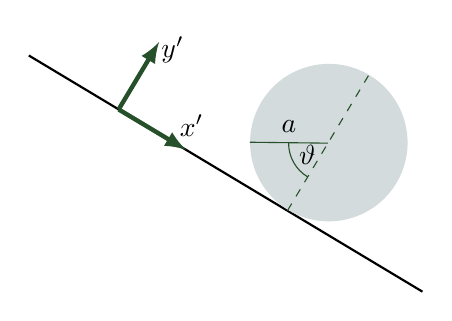
\begin{tikzpicture}
            \draw[thick] (0, 3) -- (5, 0);
            \fill[complementaryteal!20, rotate around={-31.3:(5, 0)}] (3, 1) circle [radius = 1];
            \begin{scope}[rotate around={-30.96:(5, 0)}]
                \draw[highlight, ultra thick, ->] (0.5, 0) -- (1.5, 0);
                \draw[highlight, ultra thick, ->] (0.5, 0) -- (0.5, 1);
                \node at (1.4, 0.3) {\(x'\)};
                \node at (0.7, 1) {\(y'\)};
                \draw[highlight, dashed] (3, 0) -- (3, 2);
                \draw[highlight, text=black] (3, 1) -- (2.144, 0.5) node[midway, above] {\(a\)};
                \path (2.144, 0.5) coordinate (A) -- (3, 1) coordinate (B) -- (3, 0) coordinate (C) pic [draw, "\(\vartheta\)", angle radius=0.5cm, highlight, text=black] {angle=A--B--C};
            \end{scope}
        \end{tikzpicture}
        \caption{A cylinder of radius \(a\) rolls down an inclined plane. There are initially three degrees of freedom, \(x'\), \(y'\), and \(\vartheta\), which is reduced to one degree of freedom by imposing rolling conditions.}
    \end{figure}
    
    In general each holonomic constraint decreases the number of degrees of freedom by one.
    
    \subsection{Nonholonomic Constraints}
    Unsurprisingly \defineindex{nonholonomic constraints} are those which aren't holonomic, that is they can't be written as a simple algebraic equation of the coordinates and time.
    Most often they come in the form of inequalities or differential equations.
    
    \begin{exm}{Inequality Constraint}{}
        A particle is constrained to move in a rectangular box of width \(a\) and height \(b\).
        This is a nonholonomic constraint since the constraint is equivalent to
        \begin{equation}
            0 \le x \le a, \qqand 0 \le y \le b.
        \end{equation}
        Notice that this is a two dimensional problem and as such there are initially two degrees of freedom.
        After imposing the constraint there are still two degrees of freedom.
    \end{exm}
    
    \begin{exm}{Differential Constraint}{}
        Consider a hoop of radius \(a\) rolling along a plane.
        This has five degrees of freedom, the location of the centre of the hoop, \((x, y, z)\), the angle through which the hoop is rotated, \(\varphi\), and the direction in which the hoop roles, for example the angle of this line to the \(x\)-axis, \(\vartheta\).
        
        Unlike the one-dimensional case introducing rolling constraints only reduces the number of degrees of freedom by 1.
        We have now fixed \(z = a\).
        Intuitively this is because the extra freedom of an second dimension allows us to return to the same spot with a different angle of rotation by rolling in a circle with a non-integer ratio of its radius to \(a\).
        Mathematically this is because the constraints we now have are that a small change in the angle, \(\dl{\varphi}\), corresponds to a change \(\dl{r} = a\dl{\varphi}\), where \(\dl{r}\) is a small displacement along the direction of rolling.
        Decomposing into \(x\) and \(y\) changes we have that \(\dl{x} = a\cos\vartheta\dl{\varphi}\) and \(\dl{y} = a\sin\vartheta\dl{\varphi}\).
        This gives the nonholonomic constraints
        \begin{equation}
            \dot{x} = a\dot{\varphi}\cos\vartheta, \qqand \dot{y} = a\dot{\varphi}\sin\vartheta.
        \end{equation}
        These constraints \emph{cannot} be integrated to get holonomic constraints as \(\vartheta\) is a function of time.
        
        Note that we can write the rolling constraint for the one-dimensional example in a differential equation form as \(\dot{x}' = a\dot{\vartheta}\), but this can immediately be integrated to give \(x' = a\vartheta + C\) for some constant \(C\) and so this is still a holonomic constraint.
    \end{exm}

    \begin{figure}
        \tikzsetnextfilename{rolling-in-plane}
        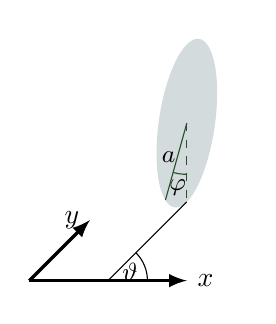
\begin{tikzpicture}
            \draw[very thick, ->] (0, 0, 2) -- (0, 0, 0) node [left] {\(y\)};
            \draw[very thick, ->] (0, 0, 2) -- (2, 0, 2) node [right] {\(x\)};
            \fill[very thick, complementaryteal!20, canvas is yz plane at x=2] (2, 2) circle [radius = 1];
            \draw[highlight, dashed, canvas is yz plane at x=2] (2, 2) -- (1, 2);
            \draw[highlight, canvas is yz plane at x=2, text=black] (2, 2) -- (2 - 1.41/2, 2 + 1.41/2);
            \node at (2, 1.8, 2.6) {{\small\(a\)}};
            \path[canvas is yz plane at x=2] (1, 2) coordinate (C) -- (2, 2) coordinate (B) -- (2 - 1.41/2, 2 + 1.41/2) coordinate (A);
            \draw pic [draw, highlight, angle radius=0.65cm] {angle};
            \node at (2, 1.3, 2.3) {{\small\(\varphi\)}};
            \draw (2, 1, 2) -- (1, 0, 2);
            \path[canvas is xz plane at y=0] (2, 2) coordinate (A) -- (1, 2) coordinate (B) -- (2, 0) pic [draw, "{\small\(\vartheta\)}"] {angle};
        \end{tikzpicture}
        \caption{A hoop rolling in the plane has five initial degrees of freedom, \(x\), \(y\), \(z\), \(\varphi\), and \(\vartheta\). Introducing rolling constraints reduces this to four degrees of freedom by fixing \(z = a\).}
    \end{figure}
    
    \chapter{Generalised Quantities}
    Often our degrees of freedom are coordinates, in particular Cartesian coordinates.
    However, this isn't always the case, for example the angle through which a body has rotated is not a Cartesian coordinate.
    Our goal in this chapter is to come up with a generalisation for several classical quantities, specifically coordinates, velocities, and force, which keep the key properties but allow us to be more general.
    We will also see generalised momentum in later chapters.
    
    \begin{ntn}{}{}
        Given some indexed quantity, \(x_i\), with \(i = 1, \dotsc, N\) we will use \(\{x\}\) as shorthand for \(x_1, x_2, \dotsc, x_N\).
    \end{ntn}

    \section{Generalised Coordinates}
    Consider some system of particles in three dimensions.
    Particle \(a\) has three coordinates, \(\vv{r_a} = (x_a, y_a, z_a)\).
    Given a list of all of the particles coordinates,
    \begin{equation}
        x_1, y_1, z_1, x_2, y_2, z_2, \dotsc, x_N, y_N, z_N,
    \end{equation}
    we have \(3N\) coordinates, for which we use the shorthand \(x_i\) with \(i = 1, \dotsc, 3N\).
    
    In the presence of holonomic constraints these \(x_i\) are not all independent.
    If we have \(M\) holonomic constraints then there are \(3N - M\) independent variables, \(q_i\), which describe the state of the system at a given time.
    We can view these as functions of the form
    \begin{equation}\label{eqn:q as func of x}
        q_i = q_i(x_1, x_2, \dotsc, x_{3N}, t) = q_i(\{x\}, t), \qquad\text{for } i = 1, \dotsc, 3N - M.
    \end{equation}
    A general aim in this course will be to generate \(3N - M\) second order differential equations in these \(q_i\).
    These are the \define{equations of motion}\index{equation of motion} (EoM)\glossary[acronym]{EoM}{equation of motion}.
    The variables \(\{q\}\) are our \define{generalised coordinates}\index{generalised coordinate}.
    
    We assume that the relation in \cref{eqn:q as func of x} is invertible and so we have
    \begin{equation}
        x_i = x_i(q_1, q_2, \dotsc, q_{3N-M}, t) = x_i(\{q\}, t), \qquad\text{for } i = 1, \dotsc, 3N.
    \end{equation}
    This allows us to recover information about the original system by solving the equations of motion for \(\{q\}\).
    The important point is that \(q_i\) can be individually varied, which we will use to derive the equations of motion, whereas we cannot vary all \(x_i\) without changing at least one other \(x_j\).
    
    \subsection{Generalised Velocities}
    The \define{generalised velocities}\index{generalised velocity} are simply the time derivatives of the generalised coordinates.
    That is, \(\dot{q}_i\), or collectively \(\{\dot{q}\}\).
    
    It should be noted that until we apply the equations of motion we can treat \(\{q\}\) and \(\{\dot{q}\}\) independently as we are considering arbitrary motion of the system.
    This means that we can just treat \(\{\dot{q}\}\) as another set of variables until we start solving the equations of motion.
    
    \section{Generalised Force}
    Consider an infinitesimal change in the coordinates, \(x_i \to x_i + \dl{x_i}\).
    This is a \defineindex{generalised displacement}.
    A simple application of the chain rule gives us
    \begin{equation}
        \dl{x_i} = \sum_j \diffp{x_i}{q_j}\dl{q_j} + \diffp{x_i}{t}\dl{t}.
    \end{equation}
    
    We define a \defineindex{virtual displacement} to be an instantaneous, infinitesimal displacement with no \(\dl{t}\) component.
    To distinguish from a normal displacement we write this as \(\delta x_i\).
    Again applying the chain rule, with the \(\dl{t}\) component vanishing, we have
    \begin{equation}
        \delta x_i = \sum_j \diffp{x_i}{q_j}\dl{q_j}.
    \end{equation}
    
    The work done in a virtual displacement due to forces \(F_i\) in the direction of \(\delta x_i\) is
    \begin{equation}
        \delta W = \sum_i F_i\delta x_i.
    \end{equation}
    We can split the force into a constraint force, and other sources of force, \(F_i^{\other}\).
    Since constraint forces do no work the work done reduces to
    \begin{equation}
        \delta W = \sum_{i} F_{i}^{\other} \delta x_i.
    \end{equation}
    We can write this in terms of \(\{\delta q\}\) using the chain rule:
    \begin{equation}
        \delta W = \sum_j \sum_i F_i^{\other} \diffp{x_i}{q_j}\delta q_j = \sum_j Q_j \delta q_j
    \end{equation}
    where we have defined the \defineindex{generalised force}
    \begin{equation}
        Q_j \coloneqq \sum_{i}F_i^{\other} \diffp{x_i}{q_j}.
    \end{equation}
    
    It should be noted that generalised quantities do not necessarily have the same dimensions as the quantity they generalise.
    For example an angle is dimensionless but may be a valid generalised coordinate, \(q\), where we would expect coordinates to have dimensions of length.
    The work done has units of energy so in this case the generalised force, \(Q\), must have units of energy so that the product \(qQ\) has units of energy.
    
    \begin{exm}{Particle on a Hoop}{exm:particle on a hoop}
        A particle of mass \(m\) slides under gravity around a smooth vertical hoop of radius \(a\).
        Taking the centre of the hoop as the origin in Cartesian coordinates we have two coordinates, \((x, z)\), to describe the position of the particle.
        We also have one holonomic constraint, that \(x^2 + z^2 = a^2\).
        Hence, there is one degree of freedom.
        
        The sensible choice for a generalised coordinate here is an angle.
        For no particular reason we choose the angle to the vertical measuring anticlockwise.
        This quantity, \(\vartheta\), is related to the Cartesian position by
        \begin{equation}
            x = -a\sin\vartheta, \qqand z = a\cos\vartheta.
        \end{equation}
    
        The force on the particle consists of a constraint force from the hoop, and the force due to gravity, \(\vv{F^{\other}} = (0, -mg)\).
        The work done on the particle in a virtual displacement, \(\delta\vartheta\), is
        \begin{align}
            \delta W &= \left[ F_x^{\other} \diffp{x}{\vartheta} + F_z^{\other} \diffp{z}{\vartheta} \right]\delta\vartheta\\
            &= 0 + (-mg)\diffp*{(a\cos\vartheta)}{\vartheta}\delta\vartheta\\
            &= (mga\sin\vartheta)\delta\vartheta.
        \end{align}
        From this we identify the generalised force
        \begin{equation}
            Q_{\vartheta} = mga\sin\vartheta.
        \end{equation}
        
        This has dimensions of energy, so \(\vartheta Q_\vartheta\) has units of energy also.
    \end{exm}
    
    \section{Functions of \texorpdfstring{\(\{q\}\), \(\{\dot{q}\}\), and \(t\)}{\{q\}, \{q-dot\}, and t}}
    We will often deal with functions of \(\{q\}\), \(\{\dot{q}\}\), and \(t\).
    For example the kinetic energy,
    \begin{equation}
        T = \sum_i \frac{1}{2}m_i\dot{x}_i^2.
    \end{equation}
    Since \(x_i = x_i(\{q\}, t)\) in generalised coordinates the kinetic energy can depend explicitly on \(\{q\}\) and \(\{\dot{q}\}\), for example in polar coordinates we saw that the kinetic energy was
    \begin{equation}
        T = \frac{1}{2}m(\dot{r}^2 + r^2\dot{\varphi}^2).
    \end{equation}
    This depends on the generalised coordinate \(r\) and the generalised velocities \(\dot{r}\) and \(\dot{\varphi}\).
    
    For such functions we can write a small increment, \(\dl{f}\), as
    \begin{equation}
        \dl{f} = \sum_j \diffp{f}{q_j} \dl{q_j} + \sum_j \diffp{f}{\dot{q}_j} \dl{\dot{q}_j} + \diffp{f}{t}\dl{t}.
    \end{equation}
    Note that we are treating \(\{q\}\) and \(\{\dot{q}\}\) as independent variables here since we have not yet imposed the equations of motion.
    
    \begin{ntn}{}{}
        When a function, \(f\), nominally depends on the variables \(a, b, c, \dotsc\) but actually is independent of a given variable, say \(b\), and we wish to emphasise this we will do so by writing \(f(a, c, \dotsc) = f(a, \nodependence{b}, c, \dotsc)\).
    \end{ntn}
    
    We now consider the special case where there is no dependence on the generalised velocities, that is \(f = f(\{q\}, t) = f(\{q\}, \nodependence{\{\dot{q}\}}, t)\).
    For this function \(\diffp{f}/{\dot{q}_j} = 0\) and so
    \begin{equation}
        \dl{f} = \sum_j \diffp{f}{q_j} \dl{q_j} + \diffp{f}{t}\dl{t}.
    \end{equation}
    This means that
    \begin{equation}
        \dot{f} = \diff{f}{t} = \sum_j \diffp{f}{q_j}\diff{q_j}{t} + \diffp{f}{t} = \sum_j \diffp{f}{q_j}\dot{q}_j + \diffp{f}{t}.
    \end{equation}
    From this we see that \(\dot{f} = \dot{f}(\{q\}, \{\dot{q}\}, t)\).
    Note that the partial derivatives of \(f\) in this expression are also independent of the velocities, the only contribution is from the \(\dl{q_j}\) terms in \(\dl{f}\):
    \begin{equation}
        \diffp{f}{q_j} = f_{q_j}(\{q\}, \nodependence{\{\dot{q}\}}, t), \qqand \diffp{f}{t} = f_t(\{q\}, \nodependence{\{\dot{q}\}}, t).
    \end{equation}
    
    Taking the partial derivative of \(\dot{f}\) with respect to \(\dot{q}_j\) we have
    \begin{equation}
        \diffp{\dot{f}}{\dot{q}_j} = \diffp*{}{q_j} \left[ \sum_j \diffp{f}{q_j}\dot{q}_j + \diffp{f}{t} \right] = \diffp{f}{q_j}.
    \end{equation}
    This gives us the so called \defineindex{cancellation of dots} rule:
    \begin{equation}\label{eqn:cancellation of dots}
        \diffp{\dot{f}}{\dot{q}_j} = \diffp{f}{q_j}.
    \end{equation}
    This \emph{only} applies if \(f\) is independent of \(\{\dot{q}\}\).
    
    Another result we will need is
    \begin{equation}\label{eqn:commuting derivatives}
        \diff*{\left( \diffp{f}{q_j} \right)}{t} = \diffp*{\left( \diff{f}{t} \right)}{q_j} = \diffp{\dot{f}}{q_j}
    \end{equation}
    referred to as the \defineindex{commuting derivatives rule}.
    
    
    \part{Lagrangian Mechanics}
    \chapter{Lagrange's Equations}
    Finally, the time has come to derive the key object of our studies in this course and also the equations that make it so useful.
    We shall do so by a method that is rather displeasing since it starts with a random quantity that just so happens to be useful.
    Later in the course we will see a derivation using the calculus of variations that doesn't require a premonition of the answer.
    
    \section{Derivation}
    We start by noting that the Cartesian coordinates are functions of the generalised coordinates and \emph{not} the generalised velocities: \(x_i = x_i(\{q\}, \nodependence{\{\dot{q}\}}, t)\).
    Because of this we can use the cancellation of dots rule (\cref{eqn:cancellation of dots}):
    \begin{equation}
        \diffp{\dot{x}_i}{\dot{q}_j} = \diffp{x_i}{q_j}.
    \end{equation}
    This holds for all \(i\) and \(j\).
    
    Now consider the magic quantity
    \begin{equation}
        \mathcal{M} = \diff{}{t}\left( m_i\dot{x}_i \diffp{\dot{x}_i}{\dot{q}_j} \right).
    \end{equation}
    Note that we are \emph{not} employing the Einstein summation convention in this course.
    
    Applying the cancellation of dots rule we get
    \begin{align}
        \mathcal{M} &= \diff{}{t} \left( m_i\dot{x}_i \diffp{x_i}{q_j} \right)\\
        &= \diff*{(m_i\dot{x}_i)}{t}\diffp{x_i}{q_j} + m_i\dot{x}_i\diff{}{t}\left( \diffp{x_i}{q_j} \right)\\
        &= \diff*{(m_i\dot{x}_i)}{t}\diffp{x_i}{q_j} + m_i\dot{x_i}\diffp{\dot{x_i}}{q_j}\\
        &= \diff*{(m_i\dot{x}_i)}{t}\diffp{x_i}{q_j} + \diff{}{q_j}\left( \frac{1}{2}m_i\dot{x}_i^2 \right).
    \end{align}
    Here we have applied the commuting derivatives rule (\cref{eqn:commuting derivatives}) since \(x_i\) has no dependence on the velocities.
    The last equality can be shown by expanding out the last derivative with the product rule.
    
    Instead of using the cancellation of dots rule we can instead write the magic quantity as
    \begin{equation}
        \mathcal{M} = \diff{}{t}\left[ \diff{}{\dot{q}_j} \left( \frac{1}{2}m_i\dot{x}_i^2 \right) \right].
    \end{equation}
    Again, this can be shown by expanding the partial derivative.
    
    Equating these two forms of the magic quantity we have
    \begin{equation}
        \mathcal{M} = \diff{}{t}\left[ \diff{}{\dot{q}_j} \left( \frac{1}{2}m_i\dot{x}_i^2 \right) \right] = \diff*{(m_i\dot{x}_i)}{t}\diffp{x_i}{q_j} + \diff{}{q_j}\left( \frac{1}{2}m_i\dot{x}_i^2 \right).
    \end{equation}
    Using Newton's second law we identify
    \begin{equation}
        \diff*{(m_i\dot{x}_i)}{t} = \dot{p}_i = F_i.
    \end{equation}
    Similarly we can identify
    \begin{equation}
        T_i = \frac{1}{2}m_i\dot{x}_i^2
    \end{equation}
    as the kinetic energy due to motion along the \(i\)th coordinate.
    Hence the magic quantity is
    \begin{equation}
        \mathcal{M} = \diff{}{t}\left( \diffp{T_i}{\dot{q}_j} \right) = F_i\diffp{x_i}{q_j} + \diffp{T_i}{q_j}.
    \end{equation}
    
    Next we sum over all \(i\).
    In doing so since derivatives are linear operators we end up with 
    \begin{equation}
        T(\{q\}, \{\dot{q}\}, t) = \sum_i T_i = \sum_i \frac{1}{2}m_i\dot{x}_i^2,
    \end{equation}
    which is the total kinetic energy.
    We can also identify
    \begin{equation}
        Q_j(\{q\}, \{\dot{q}\}, t) = \sum_i F_i\diffp{x_i}{q_j},
    \end{equation}
    the generalised force conjugate to the \(q_j\) coordinate.
    Note that the constraint forces don't contribute to this so we are free to replace \(F_i\) with \(F_i^{\other}\), the non-constraint forces.
    The constraint forces are accounted for when we reduce the number of variables by moving to generalised coordinates.
    
    Putting this all together we get
    \begin{equation}
        \diff{}{t} \left( \diffp{T}{\dot{q}_j} \right) - \diffp{T}{q_j} = Q_j.
    \end{equation}
    These\footnote{yes these, there are \(3N - M\) equations here, one for every \(j = 1, \dotsc, 3N - M\).} are \defineindex{Lagrange's equations of motion} in their most general form.
    They are derived from Newton's laws and are completely equivalent to them.
    However, it is often easier to use these equations as the constraint forces are automatically included.
    
    \begin{exm}{Particle on a Hoop}{}
        Consider the particle on a hoop from \cref{exm:particle on a hoop}.
        The particles speed is \(a\dot{\vartheta}\) and so the kinetic energy of the particle is
        \begin{equation}
            T(\vartheta, \dot{\vartheta}, t) = \frac{1}{2}ma^2 \dot{\vartheta}^2.
        \end{equation}
        We have \(\diffp{T}/{\vartheta} = 0\) and \(\diffp{T}/{\dot{\vartheta}} = ma^2\dot{\vartheta}\).
        Putting this in Lagrange's equation of motion we get
        \begin{equation}
            \diff*{(ma^2\dot{\vartheta})}{t} = mga\sin\vartheta.
        \end{equation}
        Other methods, such as conservation of energy, will give us the same result, although with more work.
    \end{exm}
    
    \section{The Lagrangian}\label{sec:the lagrangian}
    Recall that in an instantaneous virtual displacement the work done is
    \begin{equation}
        \delta W = \sum_j Q_j \delta q_j.
    \end{equation}
    Suppose we only have conservative forces.
    Then there is a potential energy function, \(V\), such that
    \begin{equation}
        \delta W = -\delta V.
    \end{equation}
    
    Suppose also that \(V = V(\{q\}, \nodependence{\{\dot{q}\}}, t)\), i.e. there is no velocity dependence\footnote{we will treat velocity dependent potentials separately later, an example of such a potential is the potential energy of an electromagnetic field for a charged particle.}.
    We then have
    \begin{equation}
        \delta W = \sum_j Q_j \delta q_j = -\delta V = -\sum_j \diffp{V}{q_j}\delta q_j.
    \end{equation}
    Since the generalised coordinates are by definition independent we can vary them individually keeping the others fixed.
    The only way to be able to do this and have the result above hold is if we have
    \begin{equation}
        Q_j = -\diffp{V}{q_j}
    \end{equation}
    for all \(j\).
    Notice the similarity to \(\vv{F} = -\grad V\), except that instead of having to consider the gradient, which becomes horrible if our coordinates are independent, such as for spherical coordinates, we can consider just single derivatives.
    
    Lagrange's equations can then be written as
    \begin{equation}
        \diff{}{t}\left( \diffp{T}{\dot{q}_j} \right) = \diffp{T}{q_j} = -\diffp{V}{q_j}.
    \end{equation}
    Since \(V = V(\{q\}, \nodependence{\{\dot{q}\}}, t)\) we have \(\diffp{V}/{\dot{q}_j} = 0\) so we are free to insert terms proportional to this at will.
    Doing so we get
    \begin{equation}
        \diff{}{t}\left( \diff{}{q_j}(T - V) \right) - \diff{}{q_j}(T - V) = 0.
    \end{equation}
    Introducing the quantity
    \begin{equation}
        \lagrangian \coloneqq T - V
    \end{equation}
    we get the form of Lagrange's equations for conservative forces with a velocity independent potential, called the \defineindex{Euler--Lagrange equations}:
    \begin{equation}
        \diff{}{t}\left( \diffp{\lagrangian}{\dot{q}_j} \right) - \diffp{\lagrangian}{q_j} = 0.
    \end{equation}
    These hold for
    \begin{equation}
        \lagrangian(\{q\}, \{\dot{q}\}, t) = T(\{q\}, \{\dot{q}\}, t) - V(\{q\}, t).
    \end{equation}
    These are the key equations of the entire course.
    
    \subsection{Notes}
    Notice the minus sign in \(\lagrangian = T - V\).
    Its not clear \emph{why} the difference between kinetic and potential energy is such a useful quantity, but it is as we shall see shortly.
    
    The time derivative is a total derivative, and therefore must be applied using the chain rule for \(f(\{q\}, \{\dot{q}\}, t)\):
    \begin{equation}
        \diff{f}{t} = \sum_j \diffp{f}{q_j}\dot{q}_j + \sum_j \diffp{f}{\dot{q}_j} \ddot{q}_j + \diffp{f}{t}.
    \end{equation}
    
    The Lagrangian is always differentiated to get the equations of motion.
    Therefore \(\lagrangian\) and \(\lagrangian + C\) will give the same equations for any constant \(C\).
    In particular we are free to ignore any additive constant in the potential energy, as we are accustomed to doing.
    
    Technically the potential we are considering, \(V(\{q\}, \nodependence{\{\dot{q}\}}, t)\), is not conservative in the standard meaning of the word as the explicit time dependence means that energy need not be conserved.
    However, the important properties of path independence apply instantaneously and this is what we used above.
    
    \subsection{Generalisations}
    There are several ways to generalise the Euler-Lagrange equations.
    We shall mention a few here.
    \begin{itemize}
        \item We have only considered holonomic constraints so far.
        We can also consider non-holonomic constraints.
        These do not decrease the degrees of freedom and instead must be imposed explicitly after solving the equations of motion.
        
        \item Not all forces are conservative, for example friction.
        Given a non-conservative force we can separate \(\{Q\}\) into conservative and non-conservative parts.
        The conservative part acts the same as it does for an entirely conservative force and we are unable to get rid of the non-conservative force through a potential so it remains:
        \begin{equation}
            \diff{}{t}\left( \diffp{\lagrangian}{\dot{q}_j} \right) - \diffp{\lagrangian}{q_j} = Q_j^{\text{non-conservative}}.
        \end{equation}
        
        Such non-conservative forces are macroscopic anyway meaning they don't appear in fundamental theories of matter and the Lagrangian formalism is well suited for these applications.
        
        \item If there are velocity dependent forces we have two choices.
        Both involve going back to the more general form of Lagrange's equations.
        We can always work directly from these but for common velocity dependent forces, such as the Lorentz force of electromagnetism, it can be advantageous to do some of the heavy lifting up front and derive a modified Lagrangian that behaves in the expected way, accounting for this velocity dependence.
        Indeed, setting up a Lagrangian is often the start point of a field theory.
    \end{itemize}
    
    \chapter{Lagrangian Methods in Action}
    \section{Single Particle}
    \subsection{Cartesian Coordinates}
    Consider an unconstrained particle in a potential \(V(\vv{r})\).
    There are three degrees of freedom.
    Taking these to be the three Cartesian coordinates we get the Lagrangian
    \begin{equation}
        \lagrangian = T - V = \sum_{i=1}^{3} \frac{1}{2}m\dot{x}_i^2 - V(\{x\}).
    \end{equation}
    We then have
    \begin{gather}
        \diffp{\lagrangian}{\dot{x}_j} = m\dot{x}_j\\
        \diffp{\lagrangian}{x_j} = \diffp{V}{x_j}\\
        \implies \diff*{(mx_j)}{t} = -\diff{V}{x_j}.
    \end{gather}
    This is simply Newton's second law with force \(\vv{F} = -\grad V\).
    Notice that if the mass is time dependent we still get the correct result.
    
    \subsection{Plane Polar Coordinates}
    Consider a particle constrained to move in a plane with a conservative potential.
    There are two degrees of freedom, which we take to be \(r\) and \(\vartheta\), the coordinates in plane polar coordinates.
    The radial velocity is \(v_r = \dot{r}\) and the tangential velocity is \(v_{\vartheta} = r\dot{\vartheta}\).
    Since these are orthogonal coordinates the velocity is just \(v = \sqrt{v_r^2 + v_\vartheta^2}\).
    Hence the Lagrangian is
    \begin{equation}
        \lagrangian = \frac{1}{2}m(\dot{r}^2 + r^2\dot{\vartheta}^2) - V(r, \vartheta).
    \end{equation}
    Considering first \(r\) we get
    \begin{gather}
        \diffp{\lagrangian}{\dot{r}} = m\dot{r},\\
        \diffp{\lagrangian}{r} = mr\dot{\vartheta} - \diffp{V}{r}.
    \end{gather}
    Assuming a time independent mass this gives us the radial equation of motion
    \begin{equation}
        m(\ddot{r} - r\dot{\vartheta}^2) = -\diff{V}{r}.
    \end{equation}
    We can identify the left hand side as \(ma_r\) where \(a_r\) is the radial acceleration.
    
    Now for \(\vartheta\) we have
    \begin{gather}
        \diffp{\lagrangian}{\dot{\vartheta}} = mr^2\dot{\vartheta} \implies \diff*{\left( \diffp{\lagrangian}{\dot{\vartheta}} \right)}{t} = 2mr\dot{r}\dot{\vartheta} + mr^2\ddot{\vartheta},\\
        \diffp{\lagrangian}{\vartheta} = -\diffp{V}{\vartheta}.
    \end{gather}
    This gives the tangential equation of motion
    \begin{equation}
        mr(2\dot{r}\dot{\vartheta} + mr\ddot{\vartheta}) = -\diffp{V}{\vartheta}.
    \end{equation}
    We can identify the left hand side as \(mra_{\vartheta}\), where \(a_{\vartheta}\) is the tangential acceleration.
    
    \section{Atwood's Machine}\label{sec:atwood's machine}
    \defineindex{Atwood's machine} is a smooth pulley with a light inextensible string.
    Attached to each end of the string is are two masses, \(m\) and \(M\).
    See \cref{fig:atwood machine}.
    
    \begin{figure}
        \tikzsetnextfilename{atwood}
        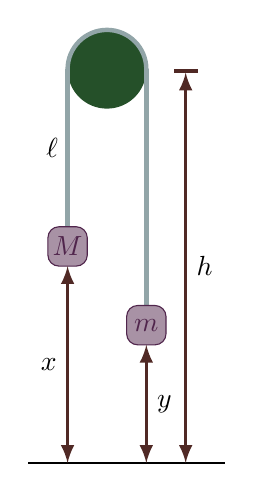
\begin{tikzpicture}
            \fill[highlight] (0, 0) circle [radius = 0.5cm];
            \draw[ultra thick, complementaryteal!50] (0.5, 0) -- ++ (0, -3);
            \draw[ultra thick, complementaryteal!50] (-0.5, 0) -- ++ (0, -2);
            \draw[ultra thick, complementaryteal!50] (0.5, 0) arc(0:180:0.5);
            \draw[rounded corners, complementarypurple, fill=complementarypurple!50] (0.25, -3) rectangle (0.75, -3.5) node[midway] {\(m\)};
            \draw[rounded corners, complementarypurple, fill=complementarypurple!50] (-0.25, -2) rectangle (-0.75, -2.5) node[midway] {\(M\)};
            \draw (-1, -5) -- (1.5, -5);
            \draw[complementaryred, <->, very thick] (0.5, -5) -- (0.5, -3.5) node[right, black, midway] {\(y\)};
            \draw[complementaryred, <->, very thick] (-0.5, -5) -- (-0.5, -2.5) node[left, black, midway] {\(x\)};
            \draw[complementaryred, <->|, very thick] (1, -5) -- (1, 0) node[right, black, midway] {\(h\)};
            \node[left] at (-0.5, -1) {\(\ell\)};
        \end{tikzpicture}
        \caption{Atwood's machine.}
        \label{fig:atwood machine}
    \end{figure}
    
    There are two degrees of freedom, we take them to be \(x\) and \(y\), the heights of \(M\) and \(m\) respectively, above some fixed floor a distance \(h\) below the pulley.
    There is one holonomic constraint:
    \begin{equation}
        x + y + \ell = 2h,
    \end{equation}
    where \(\ell\) is the length of the string\footnote{we can either assume the radius of the pulley is negligible or we can slightly redefine our coordinates to account for the part of the string that goes over the pulley.}.
    After applying this constraint we have one remaining degree of freedom.
    We take this to be \(x\).
    This lets us write
    \begin{equation}
        y = 2h - x - \ell.
    \end{equation}
    Differentiating this we have
    \begin{equation}
        \dot{y} = -\dot{x}.
    \end{equation}
    The total kinetic energy is just the kinetic energy of the two masses:
    \begin{equation}
        T = \frac{1}{2}M\dot{x}^2 + \frac{1}{2}m\dot{y}^2 = \frac{1}{2}M\dot{x}^2 + \frac{1}{2}m(-\dot{x})^2 = \frac{1}{2}(M + m)\dot{x}^2.
    \end{equation}
    The potential energy is gravitational potential energy of the two blocks, we define the floor as where the potential is zero.
    \begin{equation}
        V = Mgx + mgy = Mgx + mg(2h - x - \ell) = (M - m)gx + \text{constant}.
    \end{equation}
    Since we always differentiate the Lagrangian it is invariant under addition (or removal) of a constant term so we discard the constant.
    The Lagrangian for the system is then
    \begin{equation}
        \lagrangian = \frac{1}{2}(M - m)\dot{x}^2 - (M - m)gx.
    \end{equation}
    Hence,
    \begin{gather}
        \diffp{\lagrangian}{\dot{x}} = (M - m)\dot{x},\\
        \diffp{\lagrangian}{x} = -(M - m)g.
    \end{gather}
    Hence the equation of motion for the system is
    \begin{equation}
        (M - m)\ddot{x} = -(M - m)g \implies \ddot{x} = -\frac{M - m}{M + m}g.
    \end{equation}
    
    Notice that we don't have to consider the tension in the string, which is a real pain with the Newtonian derivation.
    
    \subsection{Atwood's Monkey}
    \defineindex{Atwood's monkey} is a modification of Atwood's machine where the mass \(M\) is replaced with a monkey of mass \(M\) which climbs up the rope at a known velocity, \(\dot{\varphi}(t)\), which is such that at time \(t\) the monkey is a distance \(\varphi(t)\) from the end of the rope.
    
    Again we initially have two degrees of freedom, \(x\) and \(y\), where now \(x\) is the distance of the monkey above the floor and \(y\) is still the height of \(m\).
    We have one holonomic constraint,
    \begin{equation}
        x + y + \ell - \varphi(t) = 2h.
    \end{equation}
    This allows us to eliminate \(y\):
    \begin{equation}
        y = 2h - x - \ell + \varphi(t).
    \end{equation}
    Differentiating this we now have
    \begin{equation}
        \dot{y} = -\dot{x} + \dot{\varphi}(t).
    \end{equation}
    The kinetic energy is then
    \begin{align}
        T &= \frac{1}{2}M\dot{x}^2 + \frac{1}{2}m\dot{y}^2\\
        &= \frac{1}{2}M\dot{x}^2 + \frac{1}{2}m(-\dot{x} + \dot{\varphi})^2\\
        &= \frac{1}{2}(M + m)\dot{x}^2 + \frac{1}{2}m\dot{\varphi}^2 - m\dot{x}\dot{\varphi}.
    \end{align}
    The potential energy is
    \begin{align}
        V &= Mgx + mgy\\
        &= Mgx + mg(2h - x - \ell + \varphi)\\
        &= (M - m)gx + mg\varphi + \text{constant}.
    \end{align}
    The Lagrangian is then
    \begin{equation}
        \lagrangian = \frac{1}{2}(M + m)\dot{x}^2 + \frac{1}{2}m\dot{\varphi}^2 - m\dot{x}\dot{\varphi} - (M - m)gx - mg\varphi.
    \end{equation}
    We then have
    \begin{gather}
        \diffp{\lagrangian}{\dot{x}} = (M + m)\dot{x} - m\dot{\varphi} \implies \diff*{\left( \diffp{\lagrangian}{\dot{x}} \right)}{t} = (M + m)\ddot{x} - m\ddot{\varphi},\\
        \diffp{\lagrangian}{x} = -(M - m)g.
    \end{gather}
    The equation of motion for the system is then
    \begin{equation}
        (M + m)\ddot{x} - m\ddot{\varphi} = -(M - m)g \implies \ddot{x} = -\frac{M - m}{M + m}g + \frac{m}{M + m}\ddot{\varphi}.
    \end{equation}
    We can integrate this to get
    \begin{equation}
        x(t) = -\frac{1}{2}\frac{M - m}{M + m}gt^2 + \frac{m}{M + m}\varphi(t) + At + B
    \end{equation}
    for constants of integration \(A\) and \(B\), which are fixed by the initial conditions.
    
    Notice that the monkey does work on the system and so energy is not conserved.
    
    \section{Particle and Wedge}
    Consider a particle on a smooth wedge, which in turn is on a smooth table.
    What is the acceleration of the wedge?
    Suppose the particle has mass \(m\), the wedge has mass \(M\), and the wedge angle is \(\varphi\).
    
    \begin{figure}
        \tikzsetnextfilename{block-wedge}
        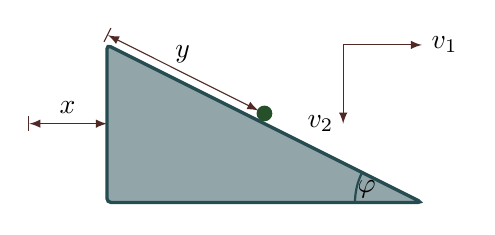
\begin{tikzpicture}
            \fill[complementaryteal!50, very thick, rounded corners=0.05cm] (0, 0) coordinate (C) -- (4, 0) coordinate (B) -- (0, 2) coordinate (A) -- cycle;
            \path pic [draw, "\(\varphi\)", angle radius=0.85cm, angle eccentricity=0.85, complementaryteal, thick, text=black] {angle};
            \draw[complementaryteal, very thick, rounded corners=0.05cm] (0, 0) -- (4, 0) -- (0, 2) -- cycle;
            \fill[highlight] (2, 1.13) circle [radius = 0.1cm];
            \draw[complementaryred, |<->] (0, 2.13) -- ++ (-26.6:2.15) node[midway, above, black] {\(y\)};
            \draw[complementaryred, |<->] (-1, 1) -- (0, 1) node[midway, above, black]  {\(x\)};
            \draw[complementaryred, <->] (4, 2) node[black, right] {\(v_1\)} -- (3, 2) -- (3, 1) node[black, left] {\(v_2\)};
        \end{tikzpicture}
        \caption{A particle on a wedge which is free to move.}
        \label{fig:particle wedge}
    \end{figure}
    
    There are two degrees of freedom.
    We choose them to be the position of the wedge and how far down the wedge the particle has slid.
    See \cref{fig:particle wedge}.
    Note that these are \emph{not} orthogonal.
    We have been asked to find out the acceleration of the wedge and we have chosen its position as one of our generalised coordinates.
    It is generally a good idea to have desired quantities as generalised coordinates.
    
    The kinetic energy has two contributions, first from the particle
    \begin{equation}
        \frac{1}{2}M\dot{x}^2,
    \end{equation}
    and from the particle,
    \begin{equation}
        \frac{1}{2}m(v_1^2 + v_2^2) = \frac{1}{2}m[(\dot{x} + \dot{y}\cos\varphi)^2 + (\dot{y}\sin\varphi)^2] = \frac{1}{2}m(\dot{x}^2 + \dot{y}^2 + 2\dot{x}\dot{y}\cos\varphi).
    \end{equation}
    The potential energy is provided by the particles gravitational potential energy, so its given by
    \begin{equation}
        V = -mgy\sin\varphi,
    \end{equation}
    taking the top of the ramp as zero potential energy.
    
    The Lagrangian for the system is
    \begin{equation}
        \lagrangian = \frac{1}{2}M\dot{x}^2 + \frac{1}{2}m(\dot{x}^2 + \dot{y}^2 + 2\dot{x}\dot{y}\cos\varphi) + mgy\sin\varphi.
    \end{equation}
    First consider \(x\):
    \begin{gather}
        \diffp{\lagrangian}{\dot{x}} = M\dot{x} + m\dot{x} + 2\dot{y}\cos\varphi \implies \diff*{\left( \diffp{\lagrangian}{\dot{x}} \right)}{t} = M\ddot{x} + m\ddot{x} + 2\ddot{y}\cos\varphi,\\
        \diffp{\lagrangian}{x} = 0.
    \end{gather}
    Hence
    \begin{equation}
        (M + m)\ddot{x} +m\ddot{y}\cos\varphi = 0.
    \end{equation}
    For \(y\) we get
    \begin{equation}
        \diffp{\lagrangian}{\dot{y}} = m\dot{y} + 2\dot{x}\cos\varphi \implies \diff*{\left( \diffp{\lagrangian}{\dot{y}} \right)}{t} = m\ddot{y} + 2\ddot{x}\cos\varphi,\\
        \diffp{\lagrangian}{y} = mg\sin\varphi,
    \end{equation}
    Hence
    \begin{equation}
        m\ddot{y} + 2\ddot{x}\cos\varphi = mg\sin\varphi.
    \end{equation}
    We now have two simultaneous equations in \(\ddot{x}\) and \(\ddot{y}\).
    Rearranging the first to give \(\ddot{y}\) and substituting into the second we can solve for \(\ddot{x}\) and we get
    \begin{equation}
        \ddot{x} = \frac{g\sin\varphi}{\cos\varphi - (m + M)\sec(\varphi)/m}.
    \end{equation}
    
    \section{Pendula}
    \subsection{Simple Pendulum}
    Consider a \defineindex{simple pendulum} consisting of a mass, \(m\), on the end of a light, rigid rod of length \(a\), fixed at the other end and constrained to move in a plane.
    Let \(\vartheta\) be the angle the pendulum makes to the vertical.
    
    \begin{figure}
        \tikzsetnextfilename{simple-pendulum}
        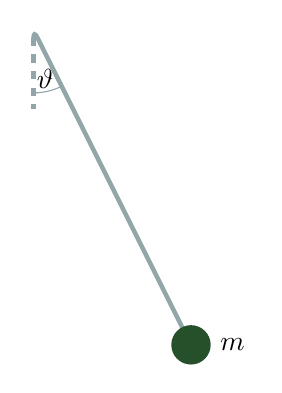
\begin{tikzpicture}
            \draw[ultra thick, complementaryteal!50, rounded corners=0.1cm] (2, -4) coordinate (C) -- (0, 0) coordinate (B) -- (0, -0.2) coordinate (A);
            \draw[ultra thick, complementaryteal!50, dashed] (0, -0.1) -- (0, -1);
            \fill[highlight] (2, -4) circle[radius=0.25cm];
            \path pic [draw, "\(\vartheta\)", angle radius=0.8cm, angle eccentricity=0.8, complementaryteal!50, text=black] {angle};
            \node[right] at (2.25, -4) {\(m\)};
        \end{tikzpicture}
        \caption{Simple pendulum.}
    \end{figure}
    
    The kinetic energy of the system is
    \begin{equation}
        T = \frac{1}{2}ma^2\dot{\vartheta}^2.
    \end{equation}
    The potential energy of the system is the gravitational potential energy of the bob.
    With a bit of trigonometry we can show that the distance of the pendulum bob below the attachment is \(a\cos\vartheta\), and hence the potential energy is
    \begin{equation}
        V = -mga\cos\vartheta.
    \end{equation}

    The Lagrangian of the system is
    \begin{equation}
        \lagrangian = \frac{1}{2}ma^2\dot{\vartheta}^2 + mga\cos\vartheta.
    \end{equation}
    Hence
    \begin{gather}
        \diffp{\lagrangian}{\dot{\vartheta}} = ma^2\dot{\vartheta} \implies \diff*{\left( \diffp{\lagrangian}{\dot{\vartheta}} \right)}{t} = ma^2\ddot{\vartheta},\\
        \diffp{\lagrangian}{\vartheta} = -mga\sin\vartheta.
    \end{gather}
    Hence the equation of motion for a pendulum is
    \begin{equation}
        ma^2\ddot{\vartheta} = -mga\sin\vartheta.
    \end{equation}
    With the small angle approximation we recover the familiar simple harmonic motion equation
    \begin{equation}
        \ddot{\vartheta} = -\omega^2\vartheta
    \end{equation}
    with \(\omega = \sqrt{g/a}\).
    
    \subsection{Spherical Pendulum}
    The \defineindex{spherical pendulum} is like the simple pendulum but no longer restricted to swing in a plane.
    Instead we have an extra degree of freedom, which we take to be the angle, \(\varphi\), about the vertical through which the pendulum swings.
    
    \begin{figure}
        \tikzsetnextfilename{spherical-pendulum}
        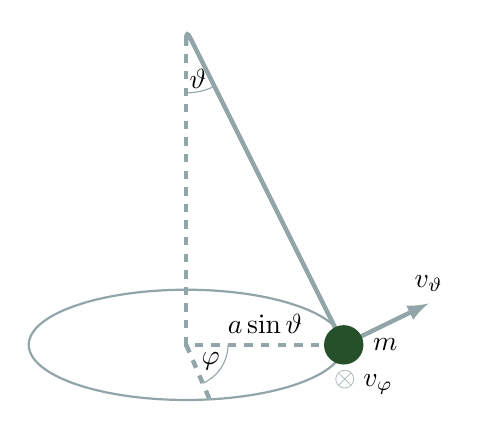
\begin{tikzpicture}
            \draw[thick, complementaryteal!50] (0, -4) circle [x radius = 2cm, y radius = 0.7cm];
            \draw[->, ultra thick, complementaryteal!50] (2, -4) -- ++ (26:1.2) node[above, black] {\(v_\vartheta\)};
            \draw[ultra thick, complementaryteal!50, rounded corners=0.1cm] (2, -4)
            coordinate (C) -- (0, 0) coordinate (B) -- (0, -0.2) coordinate (A);
            \draw[ultra thick, complementaryteal!50, dashed] (0, -0.1) -- (0, -4) -- (2, -4) node[midway, above, black] {\(a\sin\vartheta\)};
            \fill[highlight] (2, -4) circle[radius=0.25cm];
            \path pic [draw, "\(\vartheta\)", angle radius=0.8cm, angle eccentricity=0.8, complementaryteal!50, text=black] {angle};
            \draw[complementaryteal!50, ultra thick, dashed] (0, -4) coordinate (B) -- (0.3, -4.7) coordinate (A);
            \path pic [draw, "\(\varphi\)", complementaryteal!50, text=black, angle radius=0.53cm, angle eccentricity=0.7] {angle};
            \node[right] at (2.25, -4) {\(m\)};
            \node[below] at (2.25, -4.2) {\(\textcolor{complementaryteal!50}{\otimes}\;v_\varphi\)};
        \end{tikzpicture}
        \caption{Spherical Pendulum.}
    \end{figure}
    
    The kinetic energy of the pendulum is
    \begin{equation}
        T = \frac{1}{2}m(v_{\vartheta}^2 + v_{\varphi}^2)
    \end{equation}
    where \(v_{\vartheta} = a\dot{\vartheta}\) and \(v_{\varphi} = a\dot{\varphi}\sin\vartheta\), since \(a\sin\vartheta\) is the radius of the circle defined by \(\vartheta\) being constant and varying \(\varphi\).
    That is
    \begin{equation}
        T = \frac{1}{2}ma^2\dot{\varphi}^2\sin^2\vartheta + \frac{1}{2}ma^2\dot{\vartheta}^2.
    \end{equation}
    The potential energy is the same as for the simple pendulum,
    \begin{equation}
        V = -mga\cos\vartheta.
    \end{equation}

    The Lagrangian for the system is
    \begin{equation}
        \lagrangian = \frac{1}{2}ma^2\dot{\varphi}^2\sin^2\vartheta + \frac{1}{2}ma^2\dot{\vartheta}^2 + mga\cos\vartheta.
    \end{equation}
    Considering \(\vartheta\) we have
    \begin{gather}
        \diffp{\lagrangian}{\dot{\vartheta}} = ma^2\dot{\vartheta} \implies \diff*{\left( \diffp{\lagrangian}{\dot{\vartheta}} \right)}{t} = ma^2\ddot{\vartheta},\\
        \diffp{\lagrangian}{\vartheta} = ma^2\dot{\varphi}^2\sin\vartheta\cos\vartheta - mga\sin\vartheta
    \end{gather}
    giving the equation of motion
    \begin{equation}\label{eqn:spheirical pendulum theta eom}
        ma^2\ddot{\vartheta} = ma^2\dot{\varphi}^2\sin\vartheta\cos\vartheta - mgas\sin\vartheta.
    \end{equation}
    
    Now considering \(\varphi\) we have
    \begin{gather}
        \diffp{\lagrangian}{\dot{\varphi}} = ma^2\dot\varphi\sin^2\vartheta \implies \diff*{\left( \diffp{\lagrangian}{\dot{\varphi}} \right)}{t} = ma^2\ddot{\varphi}\sin^2\vartheta +2ma^2\dot{\varphi}\dot{\vartheta}\sin\vartheta\cos\vartheta\\
        \diffp{\lagrangian}{\varphi} = 0.
    \end{gather}
    Hence the equation of motion for \(\varphi\) is
    \begin{equation}\label{eqn:spherical pendulum phi eom}
        ma^2\ddot{\varphi}\sin^2\vartheta +2ma^2\dot{\varphi}\dot{\vartheta}\sin\vartheta\cos\vartheta = 0.
    \end{equation}
    
    We have two coupled differential equations.
    Integrating \cref{eqn:spherical pendulum phi eom} gives
    \begin{equation}
        ma^2\dot{\varphi}\sin^2\vartheta = \text{constant}.
    \end{equation}
    We can identify this constant as \(L_z\), the \(z\) component of the angular momentum.
    This equation implies conservation of angular momentum about the vertical axis.
    
    We can then substitute in \(\dot{\varphi}\) into \cref{eqn:spheirical pendulum theta eom} in terms of the angular momentum giving
    \begin{equation}
        ma^2\ddot{\vartheta} = ma^2\sin\vartheta\cos\vartheta \left( \frac{L_z}{a^2\sin^2\vartheta} \right)^2 - mag\sin\vartheta.
    \end{equation}
    Multiplying through by \(\dot{\vartheta}\) we can integrate both sides with respect to \(t\) which gives
    \begin{equation}
        \frac{1}{2}ma^2\dot{\vartheta}^2 = mga\cos\vartheta - \frac{L_z^2}{2ma^2\sin^2\vartheta} + \text{constant}.
    \end{equation}
    Rearranging we get
    \begin{equation}
        \frac{1}{2}ma^2\dot{\vartheta}^2 + \frac{L_z^2}{2ma^2\sin^2\vartheta} - mga\cos\vartheta = \text{constant}.
    \end{equation}
    We can identify this constant as the energy, \(E\), in particular the first two terms are the \(\vartheta\) and \(\varphi\) contributions to the kinetic energy and the last term is the potential energy.
    
    \subsubsection{Notes}
    Conservation of \(L_z\) arises because the Lagrangian is invariant under rotations about the \(z\) axis, we can see this because the Lagrangian is independent of \(\varphi\).
    This gives us a general rule
    \begin{equation}
        \diffp{\lagrangian}{q} = 0 \implies \diffp{\lagrangian}{\dot{q}} = \text{constant}.
    \end{equation}

    We will also show later that time independence of the Lagrangian (or equivalently invariance under time translations) implies conservation of energy.
    In fact every symmetry (i.e. something that leaves the Lagrangian invariant) implies a conservation law and vice versa.
    This is \defineindex{Noether's theorem}, a concept we will return to later.
    
    In this case it may have been easier to give the conservation laws by inspection:
    \begin{align}
        L_z &= ma^2 \dot{\varphi} \sin^2\vartheta = \text{constant},\\
        E &= \frac{1}{2}ma^2\dot{\vartheta}^2 + \frac{L_z^2}{2ma^2\sin^2\vartheta} - mga\cos\vartheta = \text{constant}.
    \end{align}
    This gives us two first order differential equations which are the two \define{first integrals}\index{first integral} of Lagrange's equations.
    Each symmetry will give a first integral, which gets us a fair way to solving the system.
    
    If there are as many symmetries as degrees of freedom, as is the case here, then we can often write down a set of first order differential equations like this without having to consider Lagrange's equations at all.
    We call systems where this is possible \defineindex{integrable}.
    
    \chapter{Calculus of Variations}
    \section{Functionals}
    \begin{dfn}{Functional}{}
        A \defineindex{functional} is a quantity that depends on the value of a function over some finite interval.
    \end{dfn}
    \begin{ntn}{Functionals}{}
        We typically denote functionals with capital letters, for example \(I\).
        If the functional depends on the value of the function \(y\), which is itself a function of \(s\), then we denote this either \(I[y(s)]\) or \(I[y]\), if \(s\) is obvious, with square brackets to distinguish it from a function.
    \end{ntn}
    
    Often, but not always, functionals are defined as integrals of functions.
    For example, the following are both functionals
    \begin{equation}
        I[y(s)] = \int_{s_1}^{s_2} \abs{y(s)}^2 \dd{s}, \qqand L[y(s)] = \int_{s_1}^{s_2} \sqrt{1 + \left( \diff{y}{x} \right)^2} \dd{s}.
    \end{equation}
    The following are \emph{not} functionals, they are merely functions
    \begin{equation}
        \sin(y(s)), \qqand y'(s) = \diff{y}{s}.
    \end{equation}
    Notice that the value of the derivative does depend on the value of \(y\) at both \(s\) and \(s + \dl{s}\), but for infinitesimal \(\dl{s}\) and so the interval over which \(y'\) depends on \(y\) is not finite.
    
    \section{Euler's Equation}\label{sec:Euler's equation}
    Consider a functional of the form
    \begin{equation}
        I[y(s)] = \int_a^b F(y(s), y'(s), s) \dd{s}
    \end{equation}
    where \(F\) is a function of the variables \(y\), \(y'\), and \(s\).
    We treat these as three independent variables.
    
    The \defineindex{calculus of variations} asks the question \enquote{what path, \(y\), maximises or minimises \(I[y(s)]\) subject to fixed endpoints \(y(a)\) and \(y(b)\)?}
    
    To answer this question we consider a small change in the path,
    \begin{equation}
        y(s) \to y(s) + \eta (s),
    \end{equation}
    where \(\eta(s)\) is small and vanishes at the endpoints, \(\eta(a) = \eta(b) = 0\), so that the endpoints remain fixed.
    We then answer this question by finding out when the change in \(I\) is zero, that is when
    \begin{equation}
        \delta I = I[y(s) + \eta(s)] - I[y(s)] \stackrel{?}{=} 0,
    \end{equation}
    since, as with functions, this corresponds to when the derivative is zero and hence the functional achieves some extreme value.
    
    To find this in the most general case consider
    \begin{equation}
        I[y(s) + \eta(s)] = \int_a^b F(y(s) + \eta(s), y'(s) + \eta'(s), s) \dd{s}.
    \end{equation}
    We can Taylor expand this for small \(\eta\) giving
    \begin{equation}
        I[y(s) + \eta(s)] \approx \int_a^b \left[ F(y(s), y'(s), s) + \eta(s)\diffp{F}{y} + \eta'(s)\diffp{F}{y'} \right] \dd{s}.
    \end{equation}
    Identifying the first term as \(I[y(s)]\) we see that we have
    \begin{equation}
        \delta I = \int_a^b \left[ \eta(s)\diffp{F}{y} + \eta'(s)\diffp{F}{y'} \right]\dd{s}.
    \end{equation}
    Consider the second term,
    \begin{equation}
        \int_a^b \eta'(s) \diffp{F}{y'} \dd{s}.
    \end{equation}
    Integrating by parts we get
    \begin{equation}
        \left[ \eta(s) \diffp{F}{y'} \right]_a^b - \int_a^b \eta(s)\diff*{\left( \diffp{F}{y'} \right)}{s} \dd{s} = - \int_a^b \eta(s)\diff*{\left( \diffp{F}{y'} \right)}{s} \dd{s}.
    \end{equation}
    The first term vanishes since \(\eta(a) = \eta(b) = 0\).
    We then have
    \begin{equation}
        \delta I = \int_a^b \left[ \diffp{F}{y} - \diff*{\left( \diffp{F}{y'} \right)}{s} \right] \eta(s) \dd{s}.
    \end{equation}
    We are looking for \(\delta I\) to vanish for arbitrary small changes, \(\eta\), in the path, and therefore conclude we must have
    \begin{equation}
        \diffp{F}{y} - \diff*{\left( \diffp{F}{y'} \right)}{s}.
    \end{equation}
    This is \defineindex{Euler's equation}.
    
    Notice that if we identify \(F = \lagrangian\), \(y = q\), and \(s = t\) we get Lagrange's equation.
    For this reason these two equations are often referred to as the \defineindex{Euler--Lagrange equation}.
    We will come back to what this means later.
    
    \section{First Integrals}
    Suppose that \(F\) doesn't depend on \(y\).
    From Euler's equation we have
    \begin{equation}
        \diffp{F}{y} = \implies \diff*{\left( \diffp{F}{y'} \right)}{s} = 0 \implies \diffp{F}{y'} = \text{constant.}
    \end{equation}
    
    This can often be used to to more easily solve Euler's equation.
    A similar, but less obvious, result is in the next lemma.
    
    \begin{lma}{}{}
        If \(F\) doesn't depend explicitly on \(s\), so that
        \begin{equation}
            \diffp{F}{s} = 0,
        \end{equation}
        then
        \begin{equation}
            y' \diffp{F}{y'} = F = \text{constant.}
        \end{equation}
        \begin{proof}
            Consider the total derivative
            \begin{equation}
                \diff{F}{s} = \diffp{F}{y}y' + \diffp{F}{y'}y'' + \diffp{F}{s} = \diffp{F}{y}y' + \diffp{F}{y'}y''.
            \end{equation}
            Where the final derivative vanishes by the hypothesis.
            Using Euler's equation we can substitute for the first derivative giving
            \begin{equation}
                \diff{F}{s} = \left[ \diff*{\left( \diffp{F}{y'} \right)}{s} \right]y' + \diffp{F}{y'}y''.
            \end{equation}
            Notice then that by the chain rule we have
            \begin{equation}
                \diff*{\left( \diffp{F}{y'}y' \right)}{s} = \left[ \diff*{\left( \diffp{F}{y'} \right)}{s} \right]y' + \diffp{F}{y'}y''
            \end{equation}
            and so
            \begin{equation}
                \diff{F}{s} = \diff*{\left( y'\diffp{F}{y'} \right)}{s}.
            \end{equation}
            It then follows that
            \begin{equation}
                \diff*{\left( y'\diffp{F}{y'} \right)}{s} - \diff{F}{s} = \diff{}{s}\left( y'\diffp{F}{y'} - F \right) = 0.
            \end{equation}
            From this we get the desired
            \begin{equation}
                y'\diffp{F}{y'} - F = \text{constant.}
            \end{equation}
        \end{proof}
    \end{lma}
    
    \section{Examples}
    In this section we solve a few classic calculus of variation problems.
    
    \subsection{Shortest Path}
    \textit{Given two points \((x_1, y_1)\) and \((x_2, y_2)\) in the plane what is the shortest path between them?}
    
    Suppose we have a path described by \(y(x)\), we are assuming here that the path doesn't double back on itself, which is reasonable for the shortest path, and therefore can be a function of \(x\).
    If this were not the case we would need to parametrise \(y\) and \(x\) in terms of some third variable.
    
    Consider a small step along the \(x\)-direction, \(\dl{x}\).
    If we are to stay on the path we will need to make a small step in the \(y\)-direction, \(\dl{y}\).
    The resulting step length along the path is
    \begin{equation}
        \dl{s} = \sqrt{\dl{x}^2 + \dl{y}^2} = \dl{x}\sqrt{1 + \left( \diff{y}{x} \right)^2}.
    \end{equation}
    The length of a path is then described by the functional
    \begin{equation}
        L[y(s)] = \int_{x_1}^{x_2} \dd{s} = \int_{x_1}^{x_2} \sqrt{1 + \left( \diff{y}{x} \right)^2}\dd{x} = \int_{x_1}^{x_2} \sqrt{1 + (y'(x))^2} \dd{x}.
    \end{equation}

    This is of the required form to apply Euler's equation with
    \begin{equation}
        F(y(x), y'(x), x) = \sqrt{1 + (y'(x))^2}.
    \end{equation}
    This is independent of \(y\) and so we have
    \begin{equation}
        \diffp{F}{y'} = \text{constant.}
    \end{equation}
    That is
    \begin{equation}
        \diffp{F}{y'} = \frac{y'}{\sqrt{1 + y'^2}} = p
    \end{equation}
    for some constant, \(p\).
    Inverting this we have
    \begin{equation}
        y' = \frac{p}{\sqrt{1 - p^2}} = m
    \end{equation}
    for some constant \(m\).
    Hence \(y = mx + c\), that is the shortest line between two points is a straight line.
    With the initial condition \(y(x_1) = y_1\) and \(y(x_2) = x_2\) we get \(y_1 = mx_1 + c\) and \(y_2 = mx_2 + c\).
    Subtracting one from the other we have
    \begin{equation}
        y_1 - y_2 = m(x_1 - x_2) \implies m = \frac{y_1 - y_2}{x_1 - x_2},
    \end{equation}
    which is simply the gradient of the line as expected.
    Similarly by considering \(y(0) = c\) we see that \(c\) is the \(y\)-intercept.
    
    Here we used the Euclidean metric, \(s^2 = \sum_{i,j}\delta_{ij}x_jx_i\), if instead we used a more general metric, \(s^2 = \sum_{ij} g_{ij}x_jx_i\), then we would get the general equations for a geodesic, which is just the fancy word for the shortest path in a given geometry.
    
    \subsection{Brachistochrone}
    \textit{A smooth wire connects two points, \((x_1, y_1)\) and \((x_2, y_2)\), which are in a plane with gravity acting downwards in the negative \(y\) direction. Find the path such that a bead sliding down the wire from \((x_1, y_1)\), initially at rest, reaches \((x_2, y_2)\), in the least possible time.}
    
    \begin{rmk}
        This problem was the original reason Euler invented variational calculus.
        Brachistochrone comes from the Greek \textit{\textgreek{βράχιστος}} (\textit{brákhistos}) for \textit{shortest} and \textit{\textgreek{χρόνος}} (\textit{khrónos}) for \textit{time}.
    \end{rmk}
    
    Again, we assume the path doesn't double back on itself so we look for a function \(y(x)\) which minimises the transit time, \(\tau[y(x)]\).
    In order to find the correct functional, \(\tau\), we consider the velocity at some point, \(x\), along the path..
    At \((x_1, y_1)\) the velocity is \(0\), since the particle is at rest.
    At \((x, y)\) the velocity is \(v(x)\).
    We can then apply conservation of energy and we find that
    \begin{equation}
        0 + mgy_1 = \frac{1}{2}mv^2 + mgy(x) \implies v = \sqrt{2g (y_1 - y(x))}.
    \end{equation}
    
    The time, \(\dl{\tau}\), taken to fall along a section of the path of length \(\dl{s}\) is \(\dl{\tau} = \dl{s}/v\).
    Again we have \(\dl{s} = \sqrt{1 + y'^2}\dl{x}\).
    Putting this together we have
    \begin{equation}
        \tau[y] = \int_{x_1}^{x_2} \dl{\tau} = \int_{x_1}^{x_2} \frac{1}{v}\dd{s} = \int_{x_1}^{x_2} \sqrt{\frac{1 + y'^2}{2g(y_1 - y)}} \dd{x}.
    \end{equation}
    This is of the form required to apply Euler's equation with
    \begin{equation}
        F(y(x), y'(x), x) = \sqrt{\frac{1 + y'^2}{2g(y_1 - y)}}.
    \end{equation}
    
    This has no explicit \(x\) dependence and hence
    \begin{equation}
        y'\diffp{F}{y'} - F = \text{constant.}
    \end{equation}
    We have
    \begin{equation}
        \diffp{F}{y'} = \frac{y'}{2g(y_1 - y)}\sqrt{\frac{1 + y'^2}{2g(y_1 - y)}} = \frac{Fy'}{1 + y'^2} \implies y'\diffp{F}{y'} = \frac{Fy'^2}{1 + y'^2}.
    \end{equation}
    From this we have
    \begin{equation}
        y'\diffp{F}{y'} - F = \frac{Fy'^2}{1 + y'^2} - F = -\frac{F}{1 + y'^2} = \text{constant.}
    \end{equation}
    Substituting in \(F\) and rearranging we get
    \begin{equation}
        \frac{1}{\sqrt{2g(y_1 - y)(1 + y'^2)}} = \text{constant.} \implies (y_1 - y)(1 + y'^2) = \text{constant.}
    \end{equation}
    This is the answer as far as variational calculus is concerned, a differential equation that can be solved for the path.
    Euler, being Euler, recognised it as the equation of a cycloid, which is given parametrically by
    \begin{equation}
        x = a(2\psi - \sin(2\psi)) + x_1, \qqand y = a(\cos(2\psi) - 1) + y_1
    \end{equation}
    where \(\psi\) is the angle the curve makes to the the upward vertical.
    The cycloid starts vertical, which gives a large initial acceleration, and then levels out to give a relatively short path once the ring is going quickly.
    It should be noted that a cycloid is the path traced by a point on a circle rolling along the \(x\)-axis.
    
    \begin{figure}
        \tikzsetnextfilename{brachistochrone}
        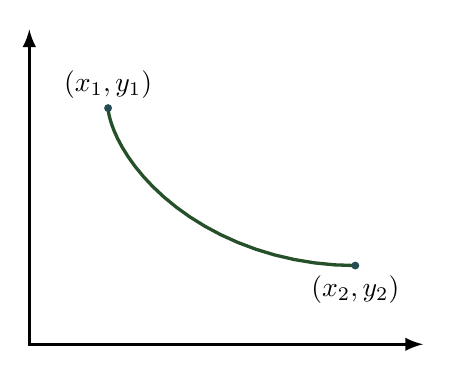
\begin{tikzpicture}
            \draw[domain=0:3.14, very thick, highlight] plot ({\x - sin(\x r) + 1}, {cos(\x r) + 2});
            \draw[very thick, ->] (0, 0) -- (0, 4);
            \draw[very thick, ->] (0, 0) -- (5, 0);
            \draw[very thick] (1, 0) -- (0, 0) -- (0, 1);
            \fill[complementaryteal] (1, 3) circle [radius=0.05cm] node[black, above] {\((x_1, y_1)\)};
            \fill[complementaryteal] (4.14, 1) circle [radius=0.05cm] node[black, below] {\((x_2, y_2)\)};
        \end{tikzpicture}
        \caption{The Brachistochrone}
    \end{figure}
    
    \subsection{Soap Film}
    \epigraph{\ldots minimise its surface area, something something, energy!}{Matt Parker on why the bubble is shaped to minimise its surface area \cite{parker2021}.}
    \epigraph{Sadly, that's super difficult}{Matt Parker, on doing this calculation \cite{parker2021}.}
    \textit{Two wire rings of radius \(a\) are held at separation \(2d\). What axially symmetric shape, \(\rho(z)\), minimises the surface area, \(A\), of a soap film connecting them?}
    
    \begin{rmk}
        Minimising the surface area gives the shape of the soap film since the surface tension acts to minimise surface area. We assume that the shape is axially symmetric and so it is only the distance from the axis at some point along the axis that we need to know.
    \end{rmk}
    
    Consider taking a small step, \(\dl{z}\), along the axis of symmetry.
    In order to stay on the soap film a small step, \(\dl{\rho}\), must be taken along the soap film.
    The resulting step along the soap film is
    \begin{equation}
        \dl{s} = \sqrt{\dl{z}^2 + \dl{\rho}^2} = \dl{z} \sqrt{1 + \rho'(z)^2}.
    \end{equation}
    Multiplying by \(2\pi\) gives the area corresponding to this range of \(z\) values and so integrating we have
    \begin{equation}
        A[\rho(z)] = \int_{z=-d}^{z=d} 2\pi \rho(z) \dd{s} = 2\pi \int_{-d}^{d} \rho\sqrt{1 + \rho'^2} \dd{z}.
    \end{equation}

    This is of form required to apply Euler's equation with
    \begin{equation}
        F(\rho(z), \rho'(z), z) = \rho\sqrt{1 + \rho'^2}.
    \end{equation}
    This has no explicit \(z\) dependence and so
    \begin{equation}
        \rho'\diffp{F}{\rho'} - F = \text{constant} = C.
    \end{equation}
    From this we get
    \begin{equation}
        \rho' \frac{\rho \rho'}{\sqrt{1 + \rho'^2}} - \rho\sqrt{1 + \rho'^2} = C.
    \end{equation}
    This can be simplified to
    \begin{equation}
        \rho = -C\sqrt{1 + \rho'^2} \implies \diff{\rho}{z} = \sqrt{\left( \frac{\rho(z)}{C} \right)^2 - 1}.
    \end{equation}
    This is the solution as far as calculus of variations is concerned.
    This can be solved by separation of variables to find
    \begin{equation}
        \rho(z) = C\cosh\left( \frac{z - z_0}{C} \right)
    \end{equation}
    where \(z_0\) is a constant of integration.
    Including the boundary condition that \(\rho(\pm d) = a\) we get \(z_0 = 0\) and hence
    \begin{equation}
        \frac{a}{C} = \cosh\left( \frac{d}{C} \right).
    \end{equation}
    This cannot he solved analytically and numerically we find it has answers only if \(d/a < 0.663\dots\).
    We interpret this as meaning that if the rings are moved too far apart then the soap film pops, and instead fills the rings in flat discs, although the mathematics would suggest an infinitely thin strand connecting the two discs along the axis, but this doesn't happen in reality.
    
    \begin{figure}
        \tikzsetnextfilename{soap-film}
        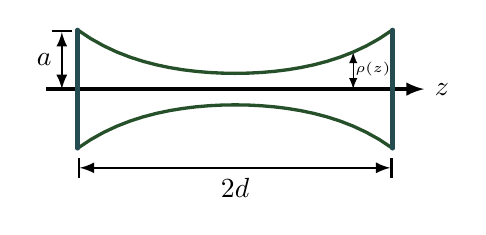
\begin{tikzpicture}
            \draw[very thick, ->] (-2.4, 0) -- (2.4, 0) node[right] {\(z\)};
            \draw[<->|, thick] (-2.2, 0) -- (-2.2, 0.752) node[left, midway] {\(a\)};
            \draw[|<->|, thick] (-2, -1) -- (2, -1) node[midway, below] {\(2d\)};
            \draw[<->] (1.5, 0) -- (1.5, 0.47);
            \node[font=\tiny] at (1.75, 0.26) {\(\rho(z)\)};
            \draw[domain=-2:2, very thick, highlight] plot (\x, {0.2*cosh(\x)});
            \draw[domain=-2:2, very thick, highlight] plot (\x, {-0.2*cosh(\x)});
            \draw[ultra thick, line cap=round, complementaryteal] (2, -0.752) -- (2, 0.752);
            \draw[ultra thick, line cap=round, complementaryteal] (-2, -0.752) -- (-2, 0.752);
        \end{tikzpicture}
        \caption{Soap film between two rings.}
    \end{figure}
    
    \section{Calculus of Variations for Many Variables}
    Now consider a functional of many paths given by
    \begin{equation}
        I[\{y(s)\}] = \int_a^b F(\{y\}, \{y'\}, s) \dd{s}.
    \end{equation}
    With \(\{y\} = y_1, y_2, \dotsc, y_p\) being a set of \(p\) linearly independent functions of the variable \(s\).
    
    Consider a small variation \(y_i \to y_i + \eta_i\), where \(\eta_i\) vanishes at the endpoints.
    We then have
    \begin{equation}
        F(\{y + \eta\}, \{y' + \eta'\}, s) \approx F(\{y\}, \{y'\}, s) + \sum_{i=1}^{p} \diffp{F}{y_i}\eta_i(s) + \sum_{i=1}^{p} \diffp{F}{y_i'}\eta_i'(s).
    \end{equation}
    Requiring that \(\delta I = 0\) and following the same derivation as the single variable case in \cref{sec:Euler's equation} we get a set of \(p\) equations, one for each \(y_i\), which are
    \begin{equation}
        \diff*{\left( \diffp{F}{y_j'} \right)}{s} - \diffp{F}{y_j} = 0.
    \end{equation}
    
    We can similarly derive first integrals the obvious one being if for some specific \(i\) \(F\) doesn't depend on \(y_i\) then we have
    \begin{equation}
        \diffp{F}{y_i'} = \text{constant.}
    \end{equation}
    There is one of these equations for each variable, \(y_i\), upon which \(F\) does not depend.
    
    If \(F\) doesn't depend on \(s\) then
    \begin{equation}\label{eqn:first integral second kind multivariable}
        \sum_i y_i'\diffp{F}{y_i'} - F = \text{constant.}
    \end{equation}
    There is only one equation here which includes all \(y_i\).
    
    \section{Hamilton's Principle}
    Earlier we commented that Lagrange's equations are just the Euler--Lagrange equations with \(F = \lagrangian\), \(y_i = q_i\), and \(s = t\).
    This implies that we can view Lagrangian mechanics as the result of demanding that the following functional is stationary:
    \begin{equation}
        S[\{q(t)\}] \coloneqq \int_{t_1}^{t_2} \lagrangian(\{q\}, \{\dot{q}\}, t) \dd{t}.
    \end{equation}
    We call this the \defineindex{action}.
    \defineindex{Hamilton's principle} states that the action is stationary, that is
    \begin{equation}
        \delta S = 0.
    \end{equation}
    
    Note that Hamilton's principle as stated here involves choosing two times, \(t_1\) and \(t_2\), and requiring that \(\delta S = 0\) while keeping \(\{q(t_1)\}\) and \(\{q(t_2)\}\) fixed.
    Our preferred boundary conditions would involve one time, \(t_1\), and fixing the initial positions, \(\{q(t_1)\}\), and velocities, \(\{\dot{q}_i(t_1)\}\).
    Fortunately we can start from Hamilton's principle, derive the Lagrange equations, and then solve them for any boundary conditions we wish, so this isn't a problem.
    
    The most general form of Hamilton's principle states that
    \begin{equation}
        \delta \int \lagrangian \dd{t} = 0,
    \end{equation}
    which is coordinate independent, and hence means that it doesn't mean what choice we make for our generalised coordinates.
    
    \subsection{Hamilton's Principle from Newtonian Mechanics}
    Consider a system of \(N\) particles in three dimensions, so we have \(3N\) degrees of freedom.
    The kinetic energy in Cartesian coordinates is
    \begin{equation}
        T = \sum_i \frac{1}{2}m_i\dot{x}_i^2.
    \end{equation}
    
    Newton's second law can then be written as
    \begin{equation}
        \sum_{i} m_i\ddot{x}_i = \diff*{\left( \diffp{T}{\dot{x}_i} \right)}{t} = -\diffp{V}{x_i}
    \end{equation}
    assuming a conservative force, and hence a potential, \(V = V(\{x\}, \nodependence{\{\dot{x}\}}, t)\).
    We can therefore write
    \begin{equation}
        \diff*{\left( \diffp{T}{\dot{x}_i} \right)}{t} = -\diffp{V}{x_i} + \diffp{T}{x_i} + \diff*{\left( \diffp{V}{\dot{x}_i} \right)}{t}
    \end{equation}
    where the two extra terms are both zero.
    Defining the Lagrangian to be \(\lagrangian \coloneqq T - V\) and rearranging this we have
    \begin{equation}
        \diff*{\left( \diffp{\lagrangian}{\dot{x}_i} \right)}{t} - \diffp{\lagrangian}{x_i} = 0.
    \end{equation}
    
    We can then construct the action
    \begin{equation}
        S = \int \lagrangian(\{x\}, \{\dot{x}\}, t) \dd{t},
    \end{equation}
    and then Hamilton's principle gives us \(\delta S = 0\) in Cartesian coordinates.
    However, Hamilton's principle is coordinate independent and so \(\delta S = 0\) holds for any choice of generalised coordinates, \(\{\tilde{q}\}\).
    We have not yet applied any constraints and so there must be \(3N\) coordinates at this stage.
    
    Suppose we have \(M\) holonomic constraints, which can be expressed in Cartesian coordinates as a set of \(M\) algebraic equalities
    \begin{equation}
        f_\alpha(\{x\}, t) = 0
    \end{equation}
    where \(\alpha = 1, \dotsc, \alpha\).
    We can then specify our choice of \(3N\) coordinates, \(\{\tilde{q}\} = (\tilde{q}_1, \tilde{q}_2, \dotsc, \tilde{q}_{3N})\), as we wish.
    We make the following choice:
    \begin{equation}
        \{\tilde{q}\} = (q_1, q_2, \dotsc, q_{3N - M}, f_1, f_2, \dotsc, f_M) = \{q, f\}.
    \end{equation}
    In other words we choose \(M\) of our constraints to be precisely the values held constant by our constraints.
    We are therefore left with \(3N - M\) generalised coordinates, \(\{q\}\), which are linearly independent of each other and of the constraints.
    
    Hamilton's principle states that for unconstrained motion we have \(\delta S = 0\) and hence
    \begin{equation}
        \delta \int \lagrangian(\{q, f\}, \{\dot{q}, \dot{f}\}, t) \dd{t} = 0.
    \end{equation}
    For constrained motion we demand that \(f_\alpha = 0\), and hence \(\dot{f}_\alpha = 0\), for all \(\alpha\).
    It then follows that if we define \(\lagrangian(\{q\}, \{\dot{q}\}, t) \coloneqq \lagrangian(\{q, 0\}, \{\dot{q}, 0\}, t)\) we have
    \begin{equation}
        \delta\int \lagrangian(\{q\}, \{\dot{q}\}, t) \dd{t}.
    \end{equation}
    
    Hence Hamilton's principle applies to constrained motion in arbitrary generalised coordinates.
    From this we can derive the Euler--Lagrange equations
    \begin{equation}
        \diff*{\left( \diffp{\lagrangian}{\dot{q}_i} \right)}{t} - \diffp{\lagrangian}{q_i} = 0.
    \end{equation}
    So we have derived the key equations for Lagrangian mechanics in a new way.
    
    This will be useful when we come to consider modifications, such as allowing velocity dependent potentials, where we will use Hamilton's principle as a starting point.
    
    \chapter{Symmetries and Conservation Laws}
    In this section we will study the Lagrangian, and Euler--Lagrange equations, and look for symmetries which leave the Lagrangian, and equations of motion, invariant.
    
    \section{Invariance Properties of the Lagrangian}
    \subsection{Invariance Under Change of Generalised Coordinates}
    Consider two sets of generalised coordinates, \(\{q\}\) and \(\{q'\}\), for the same system.
    Let \(\lagrangian = \lagrangian(\{q\}, \{\dot{q}\}, t)\) be the Lagrangian in the first set of coordinates and \(\lagrangian' = \lagrangian'(\{q'\}, \{\dot{q}'\}, t)\) the Lagrangian in the second set of coordinates.
    Numerically for the same state we have \(\lagrangian = \lagrangian'\), since both are equal to \(T - V\), which is a physical property independent of the coordinates we choose to define it.
    However, the equations of motion depend on the \emph{form} of the Lagrangian, not just its numerical value, and so we cannot just assume that being numerically equal means the same equations of motion will be produced.
    We need to prove that the two Lagrangians are \define{equivalent}\index{equivalent Lagrangians}, by which we mean they lead to the same equations of motion.
    
    \begin{thm}{Invariance of the Lagrangian Under Change of Generalised Coordinates}{}
        Consider two sets of generalised coordinates, \(\{q\}\) and \(\{q'\}\), describing the same system.
        Then the Lagrangians \(\lagrangian(\{q\}, \{\dot{q}\}, t)\) and \(\lagrangian'(\{q'\}, \{\dot{q}'\}, t)\) are equivalent.
        
        \begin{proof}
            We start with \(\lagrangian\), for which we know that the Euler--Lagrange equations hold:
            \begin{equation}
                0 = \diff*{\left( \diffp{\lagrangian}{\dot{q}_j} \right)}{t} - \diffp{\lagrangian}{q_j}.
            \end{equation}
            If we can derive the Euler--Lagrange equations but for \(\lagrangian'\), \(q'\), and \(\dot{q}'\), from this then the two Lagrangians are equivalent.
            
            For the first step notice that since \(\lagrangian\) and \(\lagrangian'\) are numerically equal we can replace \(\lagrangian\) with \(\lagrangian'\) giving
            \begin{equation}
                0 = \diff*{\left( \diffp{\lagrangian'}{\dot{q}_j} \right)}{t} - \diffp{\lagrangian'}{q_j}.
            \end{equation}
            Applying the chain rule we get
            \begin{equation}\label{eqn:invariance of lagrangian under change of generalised coords}
                0 = \diff{}{t} \bigg[ \sum_i \diffp{\lagrangian'}{\dot{q}_i'}\underbrace{\diffp{q_i'}{\dot{q}_j}}_{=0} + \sum_i \diffp{\lagrangian'}{\dot{q}_i'}\diffp{\dot{q}_i'}{\dot{q}_j}\bigg] - \sum_i \diffp{\lagrangian'}{q_i'}\diffp{q_i'}{q_j} - \sum_i \diffp{\lagrangian'}{\dot{q}_i'}\diffp{\dot{q}_i'}{q_j}.
            \end{equation}
            Noticing that we can write \(q_i' = q_i'(\{q\}, \nodependence{\{\dot{q}\}}, t)\) the first term vanishes.
            The time derivative then distributes over the second term and applying the chain rule the second term becomes
            \begin{equation}
                \left[ \diff{}{t}\diffp{\lagrangian'}{\dot{q}_i'} \right] \diffp{\dot{q}_i'}{\dot{q}_j} + \diffp{\lagrangian'}{\dot{q}_i'} \left[ \diff{}{t} \diffp{\dot{q}_i'}{\dot{q}_j} \right].
            \end{equation}
            Applying the cancellation of dots rule we have \(\diffp{\dot{q}_i'}/{\dot{q}_j} = \diffp{q_i'}/{q_j}\).
            We can also apply the commuting derivatives rule to the second term after the cancellation of dots rule giving \(\diffp{\dot{q}_i'}{q_j}\).
            Then this whole term becomes
            \begin{equation}
                \left[ \diff{}{t}\diffp{\lagrangian'}{\dot{q}_i'} \right] \diffp{q_i'}{q_j} + \diffp{\lagrangian'}{\dot{q}_i'} \diffp{\dot{q}_i'}{q_j}.
            \end{equation}
            Substituting this back into \cref{eqn:invariance of lagrangian under change of generalised coords} we have
            \begin{equation}
                0 = \sum_i\left( \left[ \diff{}{t}\diffp{\lagrangian'}{\dot{q}_i'} \right]\diffp{q_i'}{q_j} + \textcolor{highlight}{\diffp{\lagrangian'}{\dot{q}_i'}\diffp{\dot{q}_i'}{q_j}} - \diffp{\lagrangian'}{q_i'}\diffp{q_i'}{q_j} - \textcolor{highlight}{ \diffp{\lagrangian'}{\dot{q}_i'}\diffp{\dot{q}_i'}{q_j}} \right).
            \end{equation}
            Noticing that the second and third term cancel and factoring out the common \(\diffp{q_i'}{q_j}\) we get
            \begin{equation}
                0 = \sum_i\left[ \diff*{\left( \diffp{\lagrangian'}{\dot{q}_i'} \right)}{t} - \diffp{\lagrangian'}{q_i'} \right]\diffp{q_i'}{q_j}.
            \end{equation}
            Since we can vary \(q_i'\) individually and this must always hold we must have that for every \(i\)
            \begin{equation}
                \diff*{\left( \diffp{\lagrangian'}{\dot{q}_i'} \right)}{t} - \diffp{\lagrangian'}{q_i} = 0.
            \end{equation}
            These are exactly the Euler--Lagrange equations for \(\lagrangian'\) in terms of \(\{q\}\) and \(\{\dot{q}\}\).
            This proves the two Lagrangians are equivalent.
        \end{proof}
    \end{thm}
    
    \subsection{Invariance Under Addition of a Total Derivative}
    \begin{thm}{Invariance of the Lagrangian Under Addition of a Total Derivative}{}
        Let \(F = F(\{q\}, \nodependence{\{\dot{q}\}}, t)\) be a function of the generalised position and time, but not the generalised velocities.
        Then the Lagrangians \(\lagrangian\) and \(\lagrangian' = \lagrangian + \diff{F}/{t}\) are equivalent.
        \begin{proof}
            Consider the Euler--Lagrange equations for \(\lagrangian'\):
            \begin{equation}
                0 = \diff*{\left( \diffp{\lagrangian'}{\dot{q}} \right)}{t} - \diffp{\lagrangian'}{q}.
            \end{equation}
            Substituting in for the definition of \(\lagrangian'\) and using the linearity of the derivative we have
            \begin{equation}
                0 = \diff*{\left( \diffp{\lagrangian}{\dot{q}} \right)}{t} + \diff*{\left( \diffp{\dot{F}}{\dot{q}} \right)}{t} - \diffp{\lagrangian}{q} - \diffp{\dot{F}}{q}.
            \end{equation}
            Notice that since \(F\) is a function of the positions \(\dot{F}\) may be a function of the velocities.
            This means we may have \(\diffp{\dot{F}}{\dot{q}} \ne 0\).
            We can simplify this by taking the second term, applying the cancellation of dots rule and then the commuting derivatives rule which gives
            \begin{equation}
                0 = \diff*{\left( \diffp{\lagrangian}{\dot{q}} \right)}{t} + \textcolor{highlight}{\diffp{\dot{F}}{q}} - \diffp{\lagrangian}{q} - \textcolor{highlight}{\diffp{\dot{F}}{q}}.
            \end{equation}
            Noticing that the second and third terms cancel we are left with
            \begin{equation}
                0 = \diff*{\left( \diffp{\lagrangian}{\dot{q}} \right)}{t} - \diffp{\lagrangian}{q}.
            \end{equation}
            This is the Euler--Lagrange equation for \(\lagrangian\), \(q\), and \(\dot{q}\), and so \(\lagrangian\) and \(\lagrangian' = \lagrangian + \dot{F}\) are equivalent.
        \end{proof}
    \end{thm}
    
    \section{Generalised Momenta}
    \begin{dfn}{Generalised Momenta}{}
        The \defineindex{generalised momentum}, or \define{canonical momentum}\index{canonical momentum|see{generalised momentum}} conjugate to the generalised coordinate \(q\) is
        \begin{equation}
            p \coloneqq \diffp{\lagrangian}{\dot{q}}.
        \end{equation}
    \end{dfn}
    
    Using this definition we can write Lagrange's equation as
    \begin{equation}
        \diff{p}{t} = \diffp{\lagrangian}{q}.
    \end{equation}
    
    \begin{exm}{}{}
        Consider a single particle in Cartesian coordinates in a a velocity independent potential.
        We have
        \begin{equation}
            \lagrangian = \frac{1}{2}m\sum_i \dot{x}_i^2 - V(\{x\}, \nodependence{\{\dot{x}\}}, t)
        \end{equation}
        and so
        \begin{equation}
            p_i = m\dot{x}_i
        \end{equation}
        which means that the conjugate momentum of \(x_i\) is just the component of the linear momentum in the \(x_i\) direction.
    \end{exm}
    
    \begin{exm}{}{}
        Consider a rotating object.
        The kinetic energy will be of the form
        \begin{equation}
            T = T_{\mathrm{linear}} + \frac{1}{2}I\dot{\vartheta}^2
        \end{equation}
        where the linear component of the kinetic energy, \(T_{\mathrm{linear}}\), is independent of \(\dot{\vartheta}\), and \(I\) is the moment of inertia.
        For a velocity independent potential we then have
        \begin{equation}
            p_{\vartheta} = I\dot{\vartheta}
        \end{equation}
        which is the angular momentum.
    \end{exm}
    
    These two examples justify calling \(\diffp{\lagrangian}/{q}\) the generalised \emph{momentum}, however, it should be noted that \(\diffp{\lagrangian}/{q}\) cannot always be identified as a momentum.
    
    Notice that if the Lagrangian doesn't depend on a specific coordinate, \(q_j\), then \(\diffp{\lagrangian}/{q_j} = 0\) and so
    \begin{equation}
        \diff{p_j}{t} = 0 \implies p_j = \mathrm{constant}.
    \end{equation}
    So \(p_j\) is conserved.
    In this case we call \(q_j\) a \defineindex{cyclic coordinate} or \defineindex{ignorable coordinate}.
    We call the conserved momentum a \defineindex{constant of motion}.
    
    We can view \(\diffp{\lagrangian}/{q_j}\) as a symmetry of the Lagrangian meaning that we are free to change \(q_j\) by some constant amount and without changing the resulting physics.
    For example conservation of linear momentum in the \(x_i\) direction corresponds to the ability to make the translation \(x_i \to x_i + \Delta x\) without changing anything, and conservation of angular momentum when rotating about \(\ve{\vartheta}\) corresponds to the ability to make the rotation \(\vartheta \to \vartheta + \Delta \vartheta\) without changing anything.
    This leads to Noether's theorem, which informally states that every symmetry of the Lagrangian leads to a conserved quantity and vice versa.
    A more formal statement relates invariance of the Lagrangian under a given Lie group to a conserved current.
    
    \section{The Energy Function}
    \begin{dfn}{Energy Function}{}
        We define the \defineindex{energy function} as
        \begin{equation}
            h(\{q\}, \{\dot{q}\}, t) = \sum_{j} \diffp{\lagrangian}{\dot{q}_j} - \lagrangian(\{q\}, \{\dot{q}\}, t) = \sum_{j} p_j\dot{q}_j - \lagrangian.
        \end{equation}
    \end{dfn}
    
    If the Lagrangian has no explicit time dependence, so \(\lagrangian = \lagrangian(\{q\}, \{\dot{q}\}, \nodependence{t})\), then we have a first integral similar to the one in \cref{eqn:first integral second kind multivariable}, giving
    \begin{equation}
        h = \sum_{j}\dot{q}_j\diffp{\lagrangian}{\dot{q}_j} - \lagrangian = \text{constant}.
    \end{equation}
    This means that \(h\) is a conserved quantity.
    In terms of Noether's theorem this corresponds to invariance of the Lagrangian under time translation.
    
    Numerically \(h\) has the same value as the Hamiltonian, \(\hamiltonian\), but \(h\) is a function of the position, velocity, and time, whereas the Hamiltonian is a function of position, momentum, and time.
    
    \subsection{Energy Function and the Total Energy}
    As the name suggests the energy function is a generalisation of the total energy, \(E = T + V\).
    However, there are times when \(h \ne E\).
    
    It turns out that a sufficient condition for \(h = E\) is that the kinetic energy be quadratic in velocity and the potential velocity independent.
    By this we mean we can write the kinetic energy as
    \begin{equation}
        T(\{q\}, \{\dot{q}\}, t) = \frac{1}{2}\sum_i\sum_j T_{ij}(\{q\}, \nodependence{\{\dot{q}\}}, t) \dot{q}_i\dot{q}_j.
    \end{equation}
    Here \(T_{ij}\) is a symmetric matrix whose entries are a function of position and time, but not velocity.
    
    An obvious example of a quadratic energy is the a set of particles in Cartesian coordinates in which
    \begin{equation}
        T = \sum_{i}\frac{1}{2}m_i\dot{x}_i^2 \implies T_{ij} = m_i\delta_{ij}.
    \end{equation}
    
    If we have a kinetic energy that is quadratic in the velocities and a potential that is independent of the velocities then
    \begin{equation}
        p_i = \diffp{\lagrangian}{\dot{q}_i} = \diffp{T}{\dot{q}_i} = \sum_j T_{ij}\dot{q}_j
    \end{equation}
    and so it follows that
    \begin{align}
        h &= \sum_i p_i\dot{q}_i - \lagrangian\\
        &= \sum_i \sum_j T_{ij}\dot{q}_j\dot{q}_i - T + V\\
        &= 2T - T + V\\
        &= T + V\\
        &= E.
    \end{align}
    
    So we see that in systems where the kinetic energy is quadratic in the velocities (and the potential velocity independent) the energy is conserved.
    We will now study two similar examples, one where the energy is quadratic in the velocity and one where it isn't.
    
    \begin{exm}{Particle on a Rod}{}
        \textit{A particle slides on a massless rod which is fixed to a pivot at one end.
        A potential, \(V(r)\), is applied to the particle and has rotational symmetry about the pivot.
        Find the two constants of motion.}
    
        Since the rod can rotate and the particle can slide along it the particle can reach any point in the plane.
        The sensible choice of coordinates is polar coordinates.
        The Lagrangian is then
        \begin{equation}
            \lagrangian = \frac{1}{2}m(\dot{r} + r^2\dot{\vartheta}^2) - V(r).
        \end{equation}
        The generalised momenta are then
        \begin{equation}
            p_r = \diffp{\lagrangian}{\dot{r}} = m\dot{r}, \qqand p_\vartheta = \diffp{\lagrangian}{\dot{\vartheta}} = mr^2\dot{\vartheta}.
        \end{equation}
        These are exactly the radial component of linear momentum and the angular momentum about the rotation axis.
        
        The Lagrangian is independent of \(\vartheta\) and therefore \(p_{\vartheta}\) is conserved.
        
        The Lagrangian is independent of time and therefore
        \begin{equation}
            h = p_r\dot{r} + p_{\vartheta}\dot{\vartheta} - \lagrangian
        \end{equation}
        is conserved.
        Since \(T\) is quadratic in the velocities this quantity is the total energy.
    \end{exm}
    
    \begin{exm}{Particle on a Rod in Forced Motion}{}
        \textit{Consider the same set up as the previous example, but now the rod is forced to rotate at a fixed angular velocity \(\dot{\vartheta} = \omega\). Find a constant of the motion.}
        
        There is now one degree of freedom, \(r\), and the Lagrangian is
        \begin{equation}
            \lagrangian = \frac{1}{2}m(\dot{r}^2 + r^2\omega^2) - V(r).
        \end{equation}
        Since \(\omega\) is a constant the kinetic energy is \emph{not} quadratic in the velocity.
        
        The canonical momentum is
        \begin{equation}
            p_r = \diffp{\lagrangian}{\dot{r}} = m\dot{r}.
        \end{equation}
        However, now
        \begin{equation}
            \diffp{\lagrangian}{r} = mr\omega^2 - \diffp{V}{r} \ne 0
        \end{equation}
        and so the canonical momentum is not conserved\footnote{fine, technically if \(V(r) = mr^2\omega^2/2\) then \(p_r\) will be conserved, but this is just being pedantic.}, even if the potential is zero.
        Notice that the first term here is the centrifugal force due to the forced rotation.
        
        The Lagrangian has no explicit time dependence and so 
        \begin{equation}
            h = p_r\dot{r} - \lagrangian = \frac{1}{2}m(\dot{r}^2 - r^2\omega^2) + V(r)
        \end{equation}
        is conserved.
        This is \emph{not} the total energy, which is not conserved in this case.
        The total energy is
        \begin{equation}
            E = \frac{1}{2}m(\dot{r}^2 + r^2\omega^2) + V(r).
        \end{equation}
        The tangential acceleration is
        \begin{equation}
            a_{\vartheta} = r\ddot{\vartheta} + 2\dot{r}\dot{\vartheta}
        \end{equation}
        which corresponds to the constraint force
        \begin{equation}
            F = ma_{\vartheta} = 2m\dot{r}\omega
        \end{equation}
        where we have used \(\ddot{\theta} = \dot{\omega} = 0\).
        The work done on the bead is then
        \begin{equation}
            Fv_{\vartheta} = 2m\omega^2r\dot{r} = \diff*{(mr^2\omega^2)}{t}.
        \end{equation}
        We can identify this quantity as
        \begin{equation}
            \diff*{(E - h)}{t} = \diff{E}{t}
        \end{equation}
        since \(h\) is conserved.
        This accounts for the change in energy.
        
        Previously we stated that constraint forces do no work, this is only the case for virtual displacements consistent with the constraints.
        The only virtual displacement here is along the rod, which is perpendicular to \(F\).
        Constraint forces can still do work in actual motion.
    \end{exm}
    
    \section{Global Symmetries and Conservation Laws}
    In this section we develop the consequences of two global symmetries.
    By a \defineindex{global symmetry} we mean a symmetry that applies to all space, rather than just a specific system.
    We will do so by considering a system of \(N\) particles, which for sufficiently large \(N\) covers all classical systems.
    We take \(\vv{r_a}\) to be the position of the \(a\)th particle.
    
    \subsection{Homogeneity}
    We assume that space is \defineindex{homogeneous}, by this we mean that it is the same anywhere, in particular we are free to choose our origin to be any point in space.
    Movement of the origin corresponds to adding a constant to the particle positions, which we can also view as translating the entire system.
    
    If space is homogenous then the Lagrangian must be invariant under a simultaneous translation of all particles, that is the coordinate transformation
    \begin{equation}
        \vv{r_a} \to \vv{r_a} + \vv{\Delta r_a}
    \end{equation}
    for some small constant \(\vv{\Delta r} = (\Delta x, \Delta y, \Delta z)\).
    Notice that the velocity is unchanged by this translation.
    The Lagrangian changes from \(\lagrangian \to \lagrangian + \Delta\lagrangian\).
    The homogeneity of space implies that \(\Delta\lagrangian = 0\).
    
    In one dimension with a single particle then to first order in \(\Delta x\) we have
    \begin{equation}
        \Delta\lagrangian = \diffp{\lagrangian}{x} \Delta x.
    \end{equation}
    In three dimensions with a single particle then to first order in \(\Delta x_i\) we have
    \begin{equation}
        \Delta\lagrangian = \diffp{\lagrangian}{x} \Delta x + \diffp{\lagrangian}{y} \Delta y + \diffp{\lagrangian}{z} \Delta z = (\grad \lagrangian) \cdot \vv{\Delta\vv{r}}.
    \end{equation}
    For \(N\) particles in three dimensions we then have
    \begin{equation}
        \Delta\lagrangian = \sum_a (\grad[\vv{r_a}] \lagrangian) \cdot \vv{\Delta r_a} = 0
    \end{equation}
    where \(\grad[\vv{r_a}] = (\partial_{x_a}, \partial_{y_a}, \partial_{z_a})\).
    Since \(\vv{\Delta r_a}\) is arbitrary we have
    \begin{equation}
        \sum_a \grad[\vv{r_a}]\lagrangian = 0.
    \end{equation}
    
    Recalling that we can write the Euler--Lagrange equations in terms of the canonical momenta as
    \begin{equation}
        \diff{p_i}{t} = \diffp{\lagrangian}{q_i} \implies \diff{\vv{p}}{t} = \grad \lagrangian
    \end{equation}
    we find that
    \begin{equation}
        0 = \sum_{a} \diff{\vv{p_a}}{t} = \diff{\vv{P}}{t}.
    \end{equation}
    This means that the total momentum, \(\vv{P}\), is conserved.
    \begin{important}
        Homogeneity of space implies conservation of total momentum.
    \end{important}

    \subsection{Isotropy}    
    We assume that space is \defineindex{isotropic}, by this we mean that it is the same in all directions, in particular we are free to choose our axes to point in any direction.
    We can view rotations of the axes as rotations of the system by switching between active and passive transformations.
    
    If space is isotropic then the Lagrangian must be invariant under a rotation of the entire system.
    A rotation takes \(\vv{r_a} \to \vv{r_a} + \vv{\Delta r_a}\) where
    \begin{equation}
        \vv{\Delta r_a} = \vv{\Phi} \times \vv{r_a}
    \end{equation}
    with \(\vv{\Phi} = \Phi\vh{\Phi}\) representing a rotation through a small angle, \(\Phi\), about an axis \(\vh{\Phi}\).
    
    Notice that the velocity is not conserved under this since the direction changes.
    The change in velocity is
    \begin{equation}
        \vv{\Delta}\dot{\vv{r}}_{\vv{a}} = \vv{\Phi} \times \dot{\vv{r}}_{\vv{a}}.
    \end{equation}

    These rotations correspond to infinitesimal rotations but from infinitesimal rotations we can build finite rotations, and so the results of this derivation apply to any rotation.
    
    Since the velocity is not constant under this transformation the resulting change in the Lagrangian also contains a term corresponding to the change in velocity, giving
    \begin{equation}
        \Delta\lagrangian = \sum_a (\grad[\vv{r_a}]\lagrangian) \cdot \vv{\Delta r_a} + \sum_a (\grad[\dot{\vv{r}}_{\vv{a}}]) \cdot \vv{\Delta}\dot{\vv{r}}_{\vv{a}}.
    \end{equation}
    We demand that this is zero if space is isotropic.
    
    Substituting for \(\vv{\Delta r_a}\) and \(\vv{\Delta}\dot{\vv{r}}_{\vv{a}}\) we get
    \begin{equation}
        0 =  = \sum_a (\grad[\vv{r_a}]\lagrangian) \cdot (\vv{\Phi} \times \vv{r_a}) + \sum_a (\grad[\dot{\vv{r}}_{\vv{a}}]) \cdot (\vv{\Phi} \times \dot{\vv{r}}_{\vv{a}}).
    \end{equation}
    Using the Euler--Lagrange equations we have
    \begin{equation}
        \diffp{\lagrangian}{x_i} = \diff*{\left( \diffp{\lagrangian}{\dot{x}_i} \right)}{t} \implies \grad[\vv{r}] \lagrangian = \diff*{\grad[\dot{\vv{r}}]}{t} \lagrangian.
    \end{equation}
    It then follows that
    \begin{equation}
        0 =  = \sum_a \left( \diff*{\grad[\dot{\vv{r}}_{\vv{a}}] \lagrangian}{t} \right) \cdot (\vv{\Phi} \times \vv{r_a}) + \sum_a (\grad[\dot{\vv{r}}_{\vv{a}}]) \cdot (\vv{\Phi} \times \dot{\vv{r}}_{\vv{a}}).
    \end{equation}
    The final term is the scalar triple product, which follows the relation \(\vv{a} \cdot (\vv{b} \times \vv{c}) = \vv{b} \cdot (\vv{c} \times \vv{a}) = (\vv{c}\times\vv{b})\cdot\vv{a}\).
    Applying this we have
    \begin{align}
        0 &= \sum_a \left[ \vv{r_a} \times \left( \diff*{\grad[\dot{\vv{r}}_{\vv{a}}] \lagrangian}{t} \right) \right] \cdot\vv{\Phi} + \sum_a [\dot{\vv{r}}_{\vv{a}} \times (\grad[\dot{\vv{r}}_{\vv{a}}])] \cdot (\vv{\Phi} \times \dot{\vv{r}}_{\vv{a}})\\
        &= \sum_a \left[ \left( \diff*{\grad[\dot{\vv{r}}_{\vv{a}}] \lagrangian}{t} \right) \cdot ( \times \vv{r_a}) + \sum_a [\dot{\vv{r}}_{\vv{a}} \times (\grad[\dot{\vv{r}}_{\vv{a}}])] \times \dot{\vv{r}}_{\vv{a}}) \right] \cdot \vv{\Phi}
    \end{align}
    Noticing that since \(\vv{\Phi}\) is constant this is the result of applying the product rule we have
    \begin{equation}
        0 = \left[ \diff{}{t} \left( \sum_a \vv{r_a}\times (\grad[\dot{\vv{r}}_{\vv{a}}] \lagrangian) \right) \right] \cdot \vv{\Phi}.
    \end{equation}
    Since this holds for arbitrary small \(\vv{\Phi}\) we must have
    \begin{equation}
        \diff{}{t}\left( \sum_a \vv{r_a}\times (\grad[\dot{\vv{r}}_{\vv{a}}] \lagrangian) \right) = 0
    \end{equation}
    which gives
    \begin{equation}
        \sum_a \vv{r_a}\times (\grad[\dot{\vv{r}}_{\vv{a}}] \lagrangian) = \sum_{a} \vv{r_a} \times \vv{p_a} = \vv{L} = \text{constant}.
    \end{equation}
    That is the total angular momentum is conserved.
    \begin{important}
        Isotropy of space implies conservation of total angular momentum.
    \end{important}
    
    \subsection{Notes}
    We have proven the above without needing Newton's third law, which shows that conservation of total linear/angular momentum is very fundamental (assuming of course that space is homogenous and isotropic).
    
    What we have seen here is another example of Noether's theorem.
    In particular we have seen that infinitesimal symmetries give rise to global conservation laws.
    A more mathematically precise statement is that the \enquote{infinitesimal symmetries} are generators for the Lie algebra of the relevant Lie group.
    The group describing translational symmetries is \(\reals^3\), and the associated Lie algebra is \(\reals^3\) with the Lie bracket \([\vv{a}, \vv{b}] = 0\) for all \(\vv{a}, \vv{b} \in \reals^3\).
    The generators of \(\reals^3\), as a Lie group, are \(\partial_i\).
    The rotation group describing rotational symmetry is \(\specialOrthogonal(3)\), and the infinitesimal rotations we have considered are elements of the Lie algebra \(\specialOrthogonalLie(3)\), the generators of \(\specialOrthogonalLie(3)\) are \(T_i\) and satisfy the commutation relations \([T_{i}, T_{k}] = \varepsilon_{ijk}T_k\).
    
    Notice that, up to factors of \(\hbar\) and \(i\) the generators of \(\reals^3\) (associated with conservation of momentum) are the momentum operators in quantum mechanics and the generators of \(\specialOrthogonalLie(3)\) (associated with conservation of angular momentum) are the angular momentum operators.
    This hints at a deep connection between symmetries and fundamental concepts of quantum mechanics, and indeed the Lagrangian formalism can be applied to quantum mechanics to exploit this connection.
    
    \chapter{Moving Away From Newtonian Physics}
    \epigraph{Physics is not broken.}{Jenni Smillie}
    \section{Velocity-Dependent Forces}
    In \cref{sec:the lagrangian} when we derived the Euler--Lagrange equations we explicitly ruled out velocity dependent potentials to derive the Euler-Lagrange equation as a special case of the more general
    \begin{equation}
        \diff*{\left( \diffp{T}{\dot{q}} \right)}{t} - \diffp{T}{q} = Q.
    \end{equation}
    For the velocity-independent case we can find \(V = V(\{q\}, \nodependence{\{\dot{q}\}}, t)\) such that
    \begin{equation}
        Q = - \diffp{V}{q}.
    \end{equation}
    We also have \(\diffp{V}/{\dot{q}} = 0\), which we used to insert zero into the derivation.
    
    If we have velocity dependent forces however then we cannot do this.
    Suppose instead that we can find a function \(\tilde{V} = \tilde{V}(\{q\}, \{\dot{q}\}, t)\) such that
    \begin{equation}
        Q = \diff*{\left( \diffp{\tilde{V}}{\dot{q}} \right)}{t} - \diffp{\tilde{V}}{q}.
    \end{equation}
    This is such that if we substitute it in and follow the same process as deriving the original Lagrangian we get the familiar equations
    \begin{equation}
        \diff*{\left( \diffp{\lagrangian}{\dot{q}} \right)}{t} - \diffp{\lagrangian}{q},
    \end{equation}
    except now \(\lagrangian = T - \tilde{V}\).
    
    While \(\tilde{V}\) is not a potential as we normally think of them all of the important results carry over such as Hamilton's principle and conservation laws since these were derived from the form of the Euler--Lagrange equations, which is unchanged.
    
    \section{The Lorentz Force}
    \begin{rmk}
        See \cref{sec:electromagnetism} for more details on electromagnetism.
    \end{rmk}
    
    Perhaps the most important velocity dependent force is the \defineindex{Lorentz force},
    \begin{equation}
        m\ddot{\vv{r}} = \vv{F} = e(\vv{E} + \dot{\vv{r}} \times \vv{B}).
    \end{equation}
    Here \(m\) is the mass of the particle, \(e\) is its charge, \(\vv{E}\) and \(\vv{B}\) are some position and time dependent electric and magnetic fields, \(\vv{F}\) is the Lorentz force, and \(\vv{r}\) is the position of the particle.
    
    \subsection{Electromagnetic Lagrangian}
    \begin{wrn}
        In this section we use index notation and the Einstein summation convention.
    \end{wrn}
    We can now derive a Lagrangian that works with velocity dependent Lorentz force.
    We start with the following result relating the product of Levi-Civita symbols, \(\varepsilon_{ijk}\), to Kronecker deltas, \(\delta_{ij}\)\footnote{see methods of theoretical physics: vectors, tensors and continuum mechanics notes for more details}:
    \begin{equation}
        \varepsilon_{ijk}\varepsilon_{klm} = \delta_{il}\delta_{jm} - \delta_{im}\delta_{jl}.
    \end{equation}
    
    In index notation the Lorentz force has a component in the \(x_i\) direction given by
    \begin{align}
        F_i &= e\left[ \vv{E} + \dot{\vv{r}} \times \vv{B} \right]_i\\
        &= e\left[ -\grad\varphi - \diffp{\vv{A}}{t} + \dot{\vv{r}} \times (\curl \vv{A}) \right]_i
    \end{align}
    where we have substituted the fields for the potentials.
    Considering the last term we have
    \begin{align}
        [\dot{\vv{r}} \times (\curl \vv{A})]_i &= \varepsilon_{ijk}\dot{x}_j(\curl\vv{A})_k\\
        &= \varepsilon_{ijk}\dot{x}_j\varepsilon_{klm}\partial_lA_m\\
        &= \varepsilon_{ijk}\varepsilon_{klm}\dot{x}_j\partial_lA_m\\
        &= (\delta_{il}\delta_{jm} - \delta_{im}\delta_{jl})\dot{x}_j\partial_lA_m\\
        &= \dot{x}_j\partial_iA_j - \dot{x}_j\partial_jA_i.
    \end{align}
    Here \(\partial_i = \diffp{}/{x_i}\), we will also use \(\partial_t = \diffp{}/{t}\).
    With this we have \((\grad\varphi)_i = \partial_i\varphi\) and so
    \begin{equation}
        F_i = e\left[ -\partial_i\varphi - \partial_tA_i + \dot{x}_j(\partial_iA_j - \partial_jA_i) \right].
    \end{equation}
    
    We wish to identify a function, \(\tilde{V}\), such that
    \begin{equation}
        F_i = \diff*{\left( \diffp{\tilde{V}}{\dot{x}_i} \right)}{t} - \diffp{\tilde{V}}{x_i}.
    \end{equation}
    There isn't really a trick to this, it just has to be done by inspection and then verified.
    We start by noting that if we choose
    \begin{equation}
        \tilde{V} = e(\varphi - \dot{x}_jA_j)
    \end{equation}
    then we have
    \begin{equation}
        -\diffp{\tilde{V}}{x_i} = -e\partial_i\varphi + \diffp*{(\dot{x}_jA_j)}{x_i} = -e\partial_i\varphi + \dot{x}_j\partial_iA_j.
    \end{equation}
    Note that we treat \(\dot{x}_j\) and \(x_i\) as independent variables.
    This matches the first and third term of the Lorentz force.
    
    Now considering the other terms, and remembering that both the scalar and vector potential are independent of the velocity, so the only velocity dependence is in the \(\dot{x}_j\) term, we have
    \begin{align}
        \diff*{\left( \diffp{\tilde{V}}{\dot{x}_i} \right)}{t} &= e\diff{}{t}\left[ 0 - \diffp{\dot{x}_j}{\dot{x}_i}A_j \right]\\
        &= -e\diff{A_i}{t}\\
        &= -e\diffp{A_i}{x_j}\diffp{x_j}{t} - e\diffp{A_i}{t}\\
        &= -e\left[ \partial_tA_i + \dot{x}_j\partial_j A_i \right].
    \end{align}
    This matches the second and fourth terms of the Lorentz force.
    We have therefore demonstrated that \(\tilde{V}\) satisfies the necessary equations and therefore we can use the Lagrangian
    \begin{equation}
        \lagrangian = \frac{1}{2}m\dot{x}_i\dot{x}_i - e\left( \varphi - \dot{x}_iA_i \right),
    \end{equation}
    or in vector notation
    \begin{equation}
        \lagrangian = \frac{1}{2}m\sum_i \dot{x}_i^2 - e[\varphi - \dot{\vv{r}} \cdot \vv{A}].
    \end{equation}
    
    \subsection{Properties Derived from the Lagrangian}
    The canonical momentum is given by
    \begin{equation}
        p_i = \diffp{\lagrangian}{\dot{x}_i} = m\dot{x}_j + eA_j,
    \end{equation}
    or in vector form
    \begin{equation}\label{eqn:canonical momentum EM}
        \vv{p} = m\vv{v} + e\vv{A},
    \end{equation}
    which is \emph{not} equal to the mechanical momentum, \(m\vv{v}\).
    It is important that when we apply rules, such as conservation of momentum if the Lagrangian is independent of position, that we remember it is the \emph{canonical} momentum that we work with, not the mechanical momentum.
    
    The energy function is
    \begin{align}
        h &= \vv{p}\cdot\dot{\vv{r}} - \lagrangian\\
        &= [m\vv{v} + e\vv{A}] \cdot \vv{v} - \frac{1}{2}mv^2 + e(\varphi - \vv{v}\cdot\vv{A})\\
        &= \frac{1}{2}mv^2 + e\varphi.\label{eqn:energy function EM}
    \end{align}
    This quantity is conserved only if \(\lagrangian\) has no explicit time dependence.
    This requires that \(\varphi\) and \(\vv{A}\) have no explicit time dependence, and hence \(\vv{E}\) and \(\vv{B}\) cannot have any explicit time dependence.
    
    When this is the case \(h\) is conserved, and since the kinetic energy is quadratic in the velocities \(h = E\).
    This result for the energy is what we expect, it is equal to the sum of the kinetic energy and electrostatic energy.
    Remember that \(\vv{B}\) does no work since \(\vv{v} \times \vv{B}\) is perpendicular to the direction of the velocity.
    If \(\vv{B}\) is time dependent then the magnetic field still does no work but there is a term \(-\diffp{\vv{A}}/{t}\) in the electric field, which contributes to the energy, but is not accounted for in the energy function.
    
    \begin{exm}{}{}
        Consider a single particle moving in a toroidal \(\vv{B}\)-field with \(\varphi = 0\).
        Such a field has potential
        \begin{equation}
            \vv{A} = (0, 0, A_z) = (0, 0, B\rho)
        \end{equation}
        where \(\rho = \sqrt{x^2 + y^2}\).
        Find two constants of motion of the field.
        
        We note here that the magnetic field arising from this potential is
        \begin{equation}
            \vv{B} = \curl\vv{A} = \frac{B}{\rho} (y, -x, 0)
        \end{equation}
        which gives circles in the \((x, y)\)-plane.
        It should be noted that we don't actually need to compute \(\vv{B}\), we do so here only to justify calling this a toroidal field.
        
        The Lagrangian is
        \begin{equation}
            \lagrangian = \frac{1}{2}m(\dot{x}^2 + \dot{y}^2 + \dot{z}^2) + e\dot{z}A_z.
        \end{equation}
        Since \(A_z = B\sqrt{x^2 + y^2}\) has no explicit \(z\) dependence the canonical momentum in the \(z\)-direction,
        \begin{equation}
            p_z = \diffp{\lagrangian}{\dot{z}} = m\dot{z} + eB\sqrt{x^2 + y^2},
        \end{equation}
        is conserved.
        This is one constant of the motion.
        
        The Lagrangian also has no explicit time dependence, hence the energy function,
        \begin{equation}
            h = \frac{1}{2}mv^2 + e\varphi = \frac{1}{2}m(\dot{x}^2 + \dot{y}^2 + \dot{z}^2),
        \end{equation}
        is conserved.
        That is the kinetic energy is conserved, which makes sense since the \(\vv{B}\)-field can do no work to change the kinetic energy.
    \end{exm}
    
    \section{Special Relativity}
    Lagrangian methods can also be applied to special relativity\footnote{For more details on special relativity see the relativity section of the relativity, nuclear, and particle physics course.}.
    The problem we have is that in special relativity we work with the relativistic three-momentum,
    \begin{equation}
        \vv{p} = \gamma(u)m\vv{u}
    \end{equation}
    where \(m\) is the mass, \(\vv{u}\) the velocity, and \(\gamma(u) = (1 - u^2/c^2)^{-1/2}\), with \(c\) being the speed of light.
    The relativistic kinetic energy is
    \begin{equation}
        T = (\gamma - 1)mc^2.
    \end{equation}
    
    We want the canonical momentum calculated from the Lagrangian for a free particle to be the relativistic three-momentum, but this isn't what we get with \(\lagrangian = (\gamma - 1)mc^2\).
    Instead it turns out that the correct Lagrangian is
    \begin{equation}
        \lagrangian = -mc^2\sqrt{1 - \frac{u^2}{c^2}} - V(\vv{r}) = -\frac{1}{\gamma(u)}mc^2 - V(\vv{r}).
    \end{equation}
    We then have that
    \begin{equation}
        p_x = \diffp{\lagrangian}{\dot{x}} = \frac{m\dot{x}}{\sqrt{1 - u^2/c^2}} = \gamma(u)m\dot{x}.
    \end{equation}
    We then have the required \(\vv{p} = \gamma(u)m\vv{u}\).
    Using Lagrange's equations written in terms of the momentum,
    \begin{equation}
        \diff{p_i}{t} = \diffp{\lagrangian}{x_i}
    \end{equation}
    we have
    \begin{equation}
        \dot{\vv{p}} = \grad \lagrangian = -\grad V.
    \end{equation}
    This is what we would expect, so the Lagrangian gives the correct equations of motion, which justifies the choice.
    
    \section{Charged Relativistic Particle in an EM Field}
    We want to find a Lagrangian that gives the equations of motion
    \begin{equation}
        \diff{\vv{p}}{t} = \vv{F} = e(\vv{E} + \vv{u} \times \vv{B}).
    \end{equation}
    Where \(\vv{p}\) is the relativistic three-momentum.
    Fortunately we have already corrected for the velocity dependent potential and different momentum individually and both corrections hold when combined, so the correct Lagrangian is
    \begin{equation}
        \lagrangian = -\frac{1}{\gamma(u)}mc^2 - e[\varphi - \vv{u}\cdot\vv{A}].
    \end{equation}
    
    \subsection{Covariant Form}
    \begin{rmk}
        This section is non-examinable.
    \end{rmk}
    
    In special relativity we want to write everything in a covariant way using four vectors.
    Recall that the four-velocity is defined as
    \begin{equation}
        u^\mu \coloneqq \diff{x^\mu}{\tau} = \gamma(u)(c, \vv{u})
    \end{equation}
    where \(x^\mu = (ct, \vv{x})\) is the four-position and \(\tau\) is the proper time.
    We also define the four-potential as \(A^\mu \coloneqq (\varphi/c, \vv{A})\).
    Now consider the scalar product of these two quantities:
    \begin{align}
        u^\mu A_\mu = \gamma(u)c\frac{\varphi}{c} - \gamma(u)\vv{u}\cdot\vv{A} = \diff{t}{\tau}(\varphi - \vv{u}\cdot\vv{A})
    \end{align}
    where we have used
    \begin{equation}
        \diff{t}{\tau} = \gamma \impliedby \gamma\dd{\tau} = \dl{t},
    \end{equation}
    which is time dilation.
    Hence, the Lagrangian can be written in a covariant form as
    \begin{equation}
        \lagrangian = -mc^2\diff{\tau}{t} - eu^\mu A_\mu \diff{\tau}{t}.
    \end{equation}
    Using this we can write the action as
    \begin{align}
        S &\coloneqq \int \lagrangian \dd{t}\\
        &\hphantom{:}= \int \left( -mc^2\diff{\tau}{t} - eu^\mu A_\mu \diff{\tau}{t} \right)\dd{t}\\
        &\hphantom{:}= -\int (mc^2 + eu^\mu A_\mu) \dd{\tau}.
    \end{align}
    For the special case of a free particle we have
    \begin{equation}
        S = -mc^2 \int \dl{\tau},
    \end{equation}
    which is just \(-mc^2\) times the length of the world line of the particle.
    We can then apply Hamilton's principle, \(\delta S = 0\), to the action to derive the dynamics of the system.
    
    \chapter{Hamiltonian Dynamics}
    \section{Classical Mechanics Hamiltonian}
    Recall that we defined the energy function for a system of \(3N - M\) degrees of freedom as
    \begin{equation}
        h(\{q\}, \{\dot{q}\}, t) = \sum_i p_i \dot{q}_i - \lagrangian(\{q\}, \{\dot{q}\}, t)
    \end{equation}
    where
    \begin{equation}
        p_i \coloneqq \diffp{\lagrangian}{\dot{q}_i}
    \end{equation}
    are the canonical momenta.
    The energy function is numerically equal to the function we call the \defineindex{Hamiltonian}, \(\hamiltonian\), its just that this function is written in terms of the canonical momenta instead of the velocity.
    \begin{dfn}{Hamiltonian}{}
        \begin{equation}\label{eqn:hamiltonian definition}
            \hamiltonian(\{q\}, \{p\}, t) \coloneqq \sum_{i} p_i \dot{q}_i - \lagrangian(\{q\}, \{\dot{q}\}, t).
        \end{equation}
    \end{dfn}    
    \begin{exm}{}{exm:1d particle hamiltonian}
        Consider a particle moving in one dimension in a conservative, time-independent potential \(V(x)\).
        In this case we have
        \begin{equation}
            \lagrangian = \frac{1}{2}m\dot{x}^2 - V(x)
        \end{equation}
        and so
        \begin{equation}
            p = \diffp{\lagrangian}{\dot{x}} = m\dot{x} \implies \dot{x} = \frac{p}{m}
        \end{equation}
        from which we get
        \begin{equation}
            \hamiltonian = p\dot{x} - \lagrangian = p\frac{p}{m} - \left( \frac{1}{2}m\dot{x}^2 - V(x) \right) = \frac{p^2}{2m} + V(x).
        \end{equation}
        In this case we can identify \(p^2/(2m) = m\dot{x}^2/2 = T\) and so \(\hamiltonian = E = T + V\), although this will not always be the case.
    \end{exm}
    
    Consider the variation of \(\hamiltonian\) due to some arbitrary small variation in its arguments.
    The change in \(\hamiltonian\) is given by
    \begin{equation}\label{eqn:change in hamiltonian 1}
        \delta\hamiltonian = \sum_{i} \left[ \diffp{\hamiltonian}{q_i} \delta q_i + \diffp{\hamiltonian}{p_i}\delta p_i \right] + \diffp{\hamiltonian}{t}\delta t.
    \end{equation}
    We can consider the result of the same change in the definition of the Hamiltonian.
    For example, considering the first term \(p_i\dot{q}_i\) a small change \(p_i \to p_i + \delta p_i\) and \(\dot{q}_i \to \dot{q}_i + \delta q_i\) results in a change
    \begin{equation}
        (p_i + \delta p_i)(\dot{q}_i + \delta\dot{q}_i) - p_i\dot{q}_i = p_i\delta\dot{q}_i + q_i\delta p_i
    \end{equation}
    where we ignore second order terms.
    Hence
    \begin{equation}
        \delta\hamiltonian = \sum_{i} \left[ \dot{q}_i\delta p_i + p_i\delta\dot{q}_i \right] - \sum_{i} \left[ \diffp{\lagrangian}{q_i}\delta q_i + \diffp{\lagrangian}{\dot{q}_i} \delta \dot{q}_i \right] - \diffp{\lagrangian}{t}\delta t.
    \end{equation}
    Identifying \(\diffp{\lagrangian}/{\dot{q}_i} = p_i\) in the last term we see it cancels with the second term.
    We can also rewrite \(\diffp{\lagrangian}/{q_i} = \dot{p}_i\) for the third term, which is simply a statement of the Euler--Lagrange equations.
    This then reduces to
    \begin{equation}\label{eqn:change in hamiltonian 2}
        \delta\hamiltonian = \sum_{i} [\dot{q}_i\delta p_i - \dot{p}_i\delta q_i] - \diffp{\lagrangian}{t}\delta t.
    \end{equation}
    Since this must be true for any variation the coefficients of \(\delta \dot{q}_i\), \(\delta p_i\), and \(\delta t\) in \cref{eqn:change in hamiltonian 1,eqn:change in hamiltonian 2} must match, which gives us
    \begin{equation}
        \dot{q}_i = \diffp{\hamiltonian}{p_i}, \qquad \dot{p}_i = - \diffp{\hamiltonian}{q_i}, \qqand \diffp{\hamiltonian}{t} = - \diffp{\lagrangian}{t}.
    \end{equation}
    These are \defineindex{Hamilton's equations} of motion.
    We have replaced the \(3N - M\) second order Euler--Lagrange equations with \(6N - 2M + 1\) first order differential equations, the last being trivial if \(\lagrangian\) has no explicit time dependence.
    
    \begin{exm}{}{}
        Consider the one dimensional particle in a potential \(V(x)\) again.
        We saw in \cref{exm:1d particle hamiltonian} that \(\hamiltonian = p^2/(2m) + V(x)\).
        From Hamilton's equations we then get
        \begin{equation}
            \dot{x} = \diffp{\hamiltonian}{p} = \frac{p}{m}, \qquad \dot{p} = -\diffp{\hamiltonian}{x} = -V'(x), \qqand 0 = 0.
        \end{equation}
        The first of these is just the standard momentum definition, \(p = m\dot{x}\), and the second is the standard force-potential relationship, \(\vv{F} = -\grad V\), in one dimension.
    \end{exm}
    
    It is also possible to Derive Hamilton's equations from Hamilton's principle, \(\delta S = 0\), by writing the action as
    \begin{equation}
        S = \int \left[ \sum_i p_i\dot{q}_i - \hamiltonian \right] \dd{t}
    \end{equation}
    where the integrand is simply the inversion of \cref{eqn:hamiltonian definition} to give \(\lagrangian\).
    
    \begin{exm}{}{}
        Consider a charged, non-relativistic particle.
        We found in \cref{eqn:energy function EM} that the energy function was
        \begin{equation}
            h = \frac{1}{2}m\vv{v}^2 + e\varphi.
        \end{equation}
        We also saw in \cref{eqn:canonical momentum EM} that the canonical momentum is
        \begin{equation}
            \vv{p} = m\vv{v} + e\vv{A} \implies \vv{v} = \frac{1}{m}(\vv{p} - e\vv{A}).
        \end{equation}
        We can find the Hamiltonian by replacing the velocity in the energy function with the momentum, giving
        \begin{equation}
            \hamiltonian = \frac{1}{2}m\left[ \frac{1}{m}\left( \vv{p} - e\vv{A} \right) \right]^2 + e\varphi = \frac{1}{2m}\abs{\vv{p} - e\vv{A}}^2 + e\varphi.
        \end{equation}
        Notice that the vector potential, \(\vv{A}\), appears in the Hamiltonian, even though it didn't appear in the energy function.
        We can apply Hamilton's equations to this to get the Lorentz force law.
    \end{exm}
    
    \subsection{Poisson Brackets}
    Consider the arbitrary function \(\mathcal{A}\), which is a function of positions, momenta, and time.
    That is \(\mathcal{A} = \mathcal{A}(\{q\}, \{p\}, t)\).
    The total time derivative of \(\mathcal{A}\) is
    \begin{equation}
        \diff{\mathcal{A}}{t} = \sum_i \left[ \diffp{\mathcal{A}}{q_i}\dot{q}_i + \diffp{\mathcal{A}}{p_i}\dot{p}_i \right] + \diffp{\mathcal{A}}{t}.
    \end{equation}
    Applying Hamilton's equations this becomes
    \begin{equation}
        \diff{\mathcal{A}}{t} = \sum_i \left[ \diffp{\mathcal{A}}{q_i}\diffp{\hamiltonian}{p_i} - \diffp{\mathcal{A}}{p_i}\diffp{\hamiltonian}{q_i} \right] + \diffp{\mathcal{A}}{t}.
    \end{equation}
    
    \begin{dfn}{Poisson Bracket}{}
        For two functions, \(\mathcal{A}\) and \(\mathcal{B}\), which depend on position, momenta, and time, we define the \defineindex{Poisson bracket} as
        \begin{equation}
            \poissonbracket{\mathcal{A}}{\mathcal{B}} \coloneqq \sum_i \left[ \diffp{\mathcal{A}}{q_i}\diffp{\mathcal{B}}{p_i} - \diffp{\mathcal{A}}{p_i}\diffp{\mathcal{B}}{q_i} \right].
        \end{equation}
    \end{dfn}

    We see that 
    \begin{equation}\label{eqn:dA/dt = poisson bracket}
        \diff{\mathcal{A}}{t} = \poissonbracket{\mathcal{A}}{\mathcal{B}} + \diffp{\mathcal{A}}{t}.
    \end{equation}
    
    We can use the Poisson brackets to rewrite Hamilton's equations as
    \begin{equation}
        \dot{q}_i = \poissonbracket{q_i}{\hamiltonian}, \qquad \dot{p}_i = \poissonbracket{p_i}{\hamiltonian}, \qqand \diffp{\hamiltonian}{t} = - \diffp{\lagrangian}{t}.
    \end{equation}
    This is a nice way to write them as the first two equations are symmetric in their signs, although we still have to remember which order the terms in the Poisson bracket are.
    
    \section{Quantum Mechanics}
    \subsection{The Hamiltonian and Quantum Mechanics}
    \begin{rmk}
        For more details on quantum mechanics see the notes for principles of quantum mechanics.
    \end{rmk}
    Given a classical system with a corresponding Hamiltonian, \(\hamiltonian\), we can create an operator in quantum mechanics by making the replacement
    \begin{equation}
        \hamiltonian(q, p, t) \to \operator{\hamiltonian}\left( q, -i\hbar \diffp{}{q}, t \right)
    \end{equation}
    which then acts on the wave function in the position basis.
    This process is called \defineindex{canonical quantisation}.
    
    \begin{exm}{}{}
        For a single particle in one dimension we have
        \begin{equation}
            \hamiltonian = \frac{p^2}{2m} + V(x) \to \operator{\hamiltonian} = -\frac{\hbar^2}{2m}\diffp[2]{}{x} + V(x).
        \end{equation}
        For a charged particle in an electromagnetic field we have
        \begin{equation}
            \hamiltonian = \frac{1}{2m} \abs{\vv{p} - e\vv{A}}^2 + e\varphi
        \end{equation}
        and hence
        \begin{equation}
            \operator{\hamiltonian} = -\frac{\hbar^2}{2m}\laplacian - \frac{e\hbar}{2im}[2\vv{A} \cdot \grad + (\div \vv{A})] + \frac{e^2}{2m} \abs{\vv{A}}^2 + e\varphi.
        \end{equation}
        \begin{rmk}
            There is some ambiguity in this prescription.
            For example, classically \(\vv{p} \cdot \vv{A} = \vv{A} \cdot \vv{p}\), but \(\vv{A} \cdot \grad \ne \div\vv{A}\).
            This is a result of multiple quantum systems having the same classical limit.
        \end{rmk}
    \end{exm}
    
    To continue on with our quantisation we note that for two classical quantities, \(\mathcal{A}\) and \(\mathcal{B}\), we can make the same change, \(q \to q\), \(p \to =i\hbar\partial_q\), \(t \to t\), to get operators, \(\operator{\mathcal{A}}\) and \(\operator{\mathcal{B}}\) for these two quantities.
    The commutation relations for these operators follow from
    \begin{equation}
        i\hbar\poissonbracket{\mathcal{A}}{\mathcal{B}} = \commutator{\operator{\mathcal{A}}}{\operator{\mathcal{B}}},
    \end{equation}
    where
    \begin{equation}
        \commutator{\operator{\mathcal{A}}}{\operator{\mathcal{B}}} \coloneqq \operator{\mathcal{A}}\operator{\mathcal{B}} - \operator{\mathcal{B}}\operator{\mathcal{A}}
    \end{equation}
    is the \defineindex{commutator}.
    
    Multiplying \cref{eqn:dA/dt = poisson bracket} by \(i\hbar\) and then making the replacement of Poisson brackets for commutators and functions for operators we see that
    \begin{equation}
        \diff{\operator{\mathcal{A}}}{t} = \commutator{\operator{\mathcal{A}}}{\operator{\hamiltonian}} + i\hbar \diffp{\operator{\mathcal{A}}}{t}.
    \end{equation}
    This is Heisenberg's equation of motion for a quantum operator in the Heisenberg picture.
    
    \subsection{The Lagrangian and Quantum Mechanics}
    To finish of the section on quantum mechanics we note that the Lagrangian formalism can also be used in quantum mechanics.
    In this case we define the transition amplitude for a particle to travel from \(x_a\) at time \(t_a\) to \(x_b\) at time \(t_b\) as
    \begin{equation}\label{eqn:path integral}
        \braket{x_b, t_b}{x_a, t_a} = A \sum_{\text{paths}} \exp\left[ \frac{i}{\hbar} S[x(t)] \right] = \int \exp\left[ \frac{i}{\hbar} \int_{t_a}^{t_b} \lagrangian \dd{t} \right] \DL{x}
    \end{equation}
    where \(A\) is a normalisation factor, the sum is over all paths from \(x_a\) to \(x_b\), and \(S[x(t)]\) is the classical action,
    \begin{equation}
        S[x(t)] = \int_{t_a}^{t_b} \lagrangian(x, \dot{x}) \dd{t}.
    \end{equation}
    We define the integral in \cref{eqn:path integral} as the \defineindex{path integral}, from this we can derive all of the same results as we could with the more familiar operator formalism.\footnote{see the notes for the quantum theory course for more details on path integrals}
    
    In the limit of \(\hbar \to 0\), i.e. the classical limit, we see that the exponential in the path integral oscillates rapidly, unless we are near an area where the action is stationary.
    The oscillations mostly cancel out and the integral is dominated by the regions near the stationary action\footnote{this is the same logic as the method of stationary phase, discussed in the notes for methods of mathematical physics.}, i.e. where \(\delta S = 0\), so we recover Hamilton's principle.
    
    \part{Rigid Body Motion}
    \chapter{Euler's Method}
    \section{Recap}
    Recall that a rigid body is a system of \(N\) particles, labelled \(a = 1, \dotsc, N\), which have positions \(\vv{r_a} = (x_a, y_a, z_a) = (x_{a1}, x_{a2}, x_{a3})\) and masses \(m_a\).
    There is also the constraint that the distance between particles is fixed.
    That is
    \begin{equation}
        \abs{\vv{r_a} - \vv{r_b}} = \rho_{ab} = \text{constant}.
    \end{equation}
    
    These are not linearly independent constraints, in fact we have already shown that they combine to imply
    \begin{equation}
        M \ddot{\vv{R}} = \vv{F^{\ext}}, \qqand \dot{\vv{L}} = \vv{G^{\ext}}
    \end{equation}
    where \(M = \sum_a m_a\)  is the total mass, \(\vv{R} = \sum_a \vv{r_a}/M\) is the centre of mass, \(\vv{F^{\ext}}\) is the net external force on the body, \(\vv{L}\) is the total angular momentum, and \(\vv{G^{\ext}}\) is the net external torque.
    
    We also showed that
    \begin{equation}
        \vv{L} = \vv{J} + \vv{R} \times \vv{P}, \qqand T = T_{\mathrm{com}} + \frac{1}{2}MV^2
    \end{equation}
    where \(\vv{J}\) is the intrinsic angular momentum, which is independent of the choice of origin, \(\vv{P}\) is the total linear momentum, \(T\) is the total kinetic energy, \(T_{\mathrm{com}}\) is the kinetic energy in the centre-of-mass frame, and \(V = \abs{\dot{\vv{R}}}\) is the velocity of the centre of mass.
    
    Recall that we defined the centre-of-mass frame as the inertial (i.e. non-rotating) frame in which the centre of mass is stationary, but not necessarily at the origin.
    In this frame the instantaneous motion of the body is purely rotational.
    
    \section{Euler's Theorem}
    \begin{thm}{Euler's Theorem}{}
        Any displacement of a rigid body with one point fixed in space\footnote{The requirement that a point stays fixed essentially rules out translations.} can be described as a rotation about some single axis.
        \begin{proof}
            Rotations are represented by \(3\times 3\) orthogonal matrices, \(R \in \orthogonal(3)\).
            An equivalent statement of the theorem is that there is a non-zero vector, \(\vv{n}\) for which \(R\vv{n} = \vv{n}\), i.e. the vector is invariant under this particular rotation.
            This is the aforementioned \enquote{single axis} of rotation.
            This statement is equivalent to saying that \(\vv{n}\) is an eigenvector of \(\vv{n}\) with eigenvalue \(1\).
            Therefore to prove the statement it suffices to prove that all \(R\in\orthogonal(3)\) have 1 as an eigenvalue.
            
            We know that \(R \in \orthogonal(3)\), so by definition \(RR^{\trans} = R^{\trans}R = \ident\), i.e \(R^{-1} = R^{\trans}\).
            By properties of the determinant we then have
            \begin{equation}
                1 = \det(\ident) = \det(RR^\trans) = \det(R)\det(R^\trans) = [\det(R)]^2
            \end{equation}
            since \(\det(AB) = \det(A)\det(B)\) and \(\det(A^\trans) = \det A\).
            and so \(\det(R) = \pm 1\), indeed we can define \(\orthogonal(3)\) as the set of \(3\times 3\) real matrices with determinant \(\pm 1\).
            We suppose that \(R\) is a proper rotation, so \(\det(R) = 1\), that is \(R \in \specialOrthogonal(3)\).
            
            Another property of determinants is that \(\det(\lambda A) = \lambda^3\det(A)\) for a \(3\times 3\) matrix \(A\).
            Using this we have
            \begin{equation}
                \det(-A) = (-1)^3\det A = -\det A.
            \end{equation}
            Hence, since we assume \(\det R = 1\), we have \(\det R^{-1} = \det R^\trans = \det R = 1\).
            Thus,
            \begin{align}
                \det(R - \ident) &= \det((R - \ident)^{\trans})\\
                &= \det(R^\trans - \ident)\\
                &= \det(R^{-1} - R^{-1}R)\\
                &= \det(R^{-1}(\ident - R))\\
                &= \det(R^{-1})\det(\ident - R)\\
                &= \det(\ident - R)\\
                &= \det(-(R - \ident))\\
                &= -\det(R - \ident).
            \end{align}
            Hence \(\det(R - \ident) = 0\).
            This is equivalent to stating that \(1\) is an eigenvalue of \(R\), and so we are finished.
        \end{proof}
    \end{thm}
    Note that this theorem only works in odd dimensions, since we used the dimension of the space in the \(\det(\lambda A) = \lambda^3\det(A)\) step to get a negative.
    
    To specify a rotation we need 6 degrees of freedom:
    \begin{itemize}
        \item 2 degrees of freedom to specify the axis of rotation (we can either give its angle to the \(x\) and \(z\) axis (as in spherical polars) or a unit vector, which is two degrees of freedom since the three degrees of freedom of a vector are reduced to two by the requirement of unit modulus).
        \item 1 degree of freedom to specify the size of rotation, i.e. the angle through which the object is rotated.
        \item 3 degrees of freedom to specify the fixed position.
    \end{itemize}
    There are other ways to specify rotations, which we will come to later, but the number of degrees of freedom are the same.
    
    The velocity of the system also has six degrees of freedom, typically given as the velocity of the centre of mass, \(\dot{\vv{R}}\), and angular velocity, \(\vv{\omega}\).
    Note that we \emph{cannot} use the quantity \(\vv{\Omega}(t) = \int_0^t \vv{\omega}(t') \dd{t'}\) as a generalised coordinate, in the way we use \(\vv{R}(t) = \int_{0}^{t} \dot{\vv{R}}(t') \dd{t'}\), since rotations don't commute and it is possible that multiple rotations will give the same value for \(\vv{\Omega}(t)\).
    We will solve this problem later.
    
    \section{The Inertia Tensor}
    In the centre-of-momentum frame, taking the origin as the centre-of-mass the instantaneous velocity of the \(a\)th particle is
    \begin{equation}
        \dot{\vv{r}}_a = \vv{\omega}(t) \times \vv{r_a}.
    \end{equation}
    The intrinsic angular momentum is then
    \begin{align}
        \vv{J} &= \sum_{a} \vv{r_a} \times \vv{p_a}\\
        &= \sum_{a} m_a (\vv{r_a} \times \dot{\vv{r}}_{\vv{a}})\\
        &= \sum_{a} m_a (\vv{r_a} \times (\vv{\omega} \times \vv{r_a}))\\
        &= \sum_{a} m_ar_a^2\vv{\omega} - \sum_{a} m_a \vv{r_a} (\vv{r_a} \cdot \vv{\omega}).\label{eqn:J = Iomeag}
    \end{align}
    We have used \(\dot{\vv{r}}_{\vv{a}} = \vv{\omega} \times \vv{r_a}\) and the triple vector identity
    \begin{equation}
        \vv{a} \times (\vv{b} \times \vv{c}) = (\vv{a} \cdot \vv{c}) \vv{b} - (\vv{a} \cdot \vv{b}) \vv{c}.
    \end{equation}
    
    Here we have derived an relation between \(\vv{J}\) and \(\vv{\omega}\) that is linear in \(\vv{\omega}\), but where \(\vv{J}\) doesn't necessarily point in the direction of \(\vv{\omega}\) since the second sum is in the direction of \(\vv{r_a}\) and is in general non-zero and not in the direction of \(\vv{\omega}\).
    A linear relation that changes the direction of the vector can be encoded in a rank 2 tensor as
    \begin{equation}
        \vv{J} = I \vv{\omega}, \qquad \text{or} \qquad J_i = \sum_{j=1}^{3} I_{ij}\omega_j.
    \end{equation}
    We call \(I\) the \defineindex{inertia tensor}.
    In Cartesian coordinates by writing out the components of \cref{eqn:J = Iomeag} as
    \begin{equation}
        J_i = \sum_a m_a r_a^2 \omega_i - \sum_a m_a x_{ai} \sum_j x_{ai}\omega_j.
    \end{equation}
    From which we can identify the Cartesian components are
    \begin{equation}\label{eqn:inertia tensor componentns}
        I_{ij} = \sum_{a} m_a [r_a^2 \delta_{ij} - x_{ai}x_{aj}].
    \end{equation}
    Writing this out in a matrix we have
    \begin{equation}
        I = \sum_a m_a 
        \begin{pmatrix}
            y_a^2 + z_a^2 & -x_ay_a & -x_az_a\\
            -x_ay_a & x_a^2 + z_a^2 & -y_az_a\\
            -x_ay_a & -y_az_a & x_a^2 + y_z^2
        \end{pmatrix}
        .
    \end{equation}
    
    This explicitly involves the particle coordinates which are measured relative to the centre of mass.
    For a rigid body we can take these coordinates to be constants in the frame of reference in which the body is completely stationary, called the \defineindex{body frame}.
    This may not be an inertial frame if the body is accelerating, however it is still useful to evaluate the inertia tensor in this frame.
    
    In the centre of momentum frame the kinetic energy is
    \begin{equation}
        T = \sum_a \frac{1}{2}m_a(\vv{\omega} \times \vv{r_a}) \cdot (\vv{\omega} \times \vv{r_a}).
    \end{equation}
    Applying the scalar triple product identity, \((\vv{a} \times \vv{b}) \cdot \vv{c} = \vv{a} \cdot (\vv{b} \times \vv{c})\), we get
    \begin{equation}
        T = \frac{1}{2}\vv{\omega} \cdot \sum_a m_a \vv{r_a} \times (\vv{\omega} \times \vv{r_a}) = \frac{1}{2}\vv{\omega} \cdot \vv{J} = \frac{1}{2}\vv{\omega} \cdot I\vv{\omega}.
    \end{equation}
    
    The inertia tensor is symmetric, and hence there exist real eigenvalues, \(\{I_i\}\), which we call the \defineindex{principle moments of inertia}, and mutually orthogonal eigenvectors, \(\{\ve{i}\}\), which we take to be normalised.
    We define the \(\ve{i}\)-axes as the \defineindex{principle axes} (PA)\glossary[acronym]{PA}{principle axes}.
    In the \(\{\ve{i}\}\) basis the inertia tensor is diagonal:
    \begin{equation}
        I = 
        \begin{pmatrix}
            I_1 & 0 & 0\\
            0 & I_2 & 0\\
            0 & 0 & I_3
        \end{pmatrix}
        .
    \end{equation}
    In this basis the intrinsic angular momentum is given by
    \begin{equation}
        \vv{J} = (I_1\omega_1, I_2\omega_2, I_3\omega_3),
    \end{equation}
    and the kinetic energy by
    \begin{equation}
        T = \frac{1}{2}(I_1\omega_1^2 + I_2\omega_2^2 + I_3\omega_3^2)
    \end{equation}
    which is the centre-of-mass kinetic energy since the principle-axes frame is a centre of momentum frame.
    
    \section{Other Origins}
    So far we have considered the origin, \(O\), to be the centre of mass.
    This is a good choice for a body undergoing arbitrary rotations, since there is no other special point to pick.
    A common case however is of a body in which some other point, \(O'\), is fixed.
    The most common example being a spinning top which has its point of contact with the table fixed (of course, real spinning tops tend to move about as well but we aren't considering translations here).
    
    The total angular momentum about \(O'\) is
    \begin{equation}
        \vv{L} = \vv{J} + \vv{R} \times \vv{P}
    \end{equation}
    where \(\vv{J}\) is the angular momentum about \(O\), \(\vv{R}\) is the centre of mass, and \(\vv{P}\) is the total linear momentum.
    Notice that in the case of \(O = O'\) this reduces to \(\vv{L} = \vv{J}\) since \(\vv{R} = \vv{0}\).
    Euler's theorem, that there is a single axis of rotation, still holds and we have
    \begin{equation}
        \vv{L} = I'\vv{\omega},
    \end{equation}
    where \(I'\) is the momentum of inertia tensor taking \(O'\) as te origin.
    We can find this by changing the coordinates in the definition of \(I_{ij}\) (\cref{eqn:inertia tensor componentns}).
    To do so we use \(\vv{r_a} = \vv{d} + \vv{r_a}'\) where \(\vv{r_a}\) is the position relative to \(O\), \(\vv{r_a}'\) is the position relative to \(O'\), and \(\vv{d}\) is the constant displacement of \(O'\) relative to \(O\), all of these quantities being in the body frame, and so don't change as the object rotates.
    See \cref{fig:inertia tensor shifted origin}.
    
    \begin{figure}
        \tikzsetnextfilename{shifted-origin-inertia-tensor-coords}
        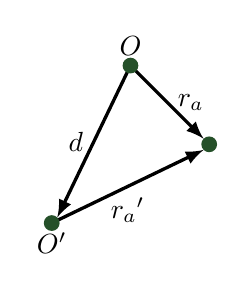
\begin{tikzpicture}
            \draw[very thick, ->] (0, 0) -- ($(2, 1) + (-135:0.1)$) node[midway, below] {\(\vv{r_a}'\)};
            \draw[very thick, ->] (1, 2) -- ($(0, 0) + (45:0.1)$) node[midway, left] {\(\vv{d}\)};
            \draw[very thick, ->] (1, 2) -- ($(2, 1) + (135:0.1)$) node[midway, right] {\(\vv{r_a}\)};
            \fill[highlight] (0, 0) circle [radius = 0.1cm] node[below, black] {\(O'\)};
            \fill[highlight] (1, 2) circle [radius = 0.1cm] node[above, black] {\(O\)};
            \fill[highlight] (2, 1) circle [radius = 0.1cm];
        \end{tikzpicture}
        \caption{The relationship between the two origins, \(O\) and \(O'\), and some arbitrary point.}
        \label{fig:inertia tensor shifted origin}
    \end{figure}
    
    The kinetic energy, including that of the centre of mass motion in the principle axis basis, is then given by
    \begin{equation}
        T = \frac{1}{2}\vv{\omega} \cdot I' \vv{\omega} = \frac{1}{2}(I_1'\omega_1^2 + I_2\omega_2^2 + I_3\omega_3^2).
    \end{equation}
    
    One common use case is when \(O'\) is a distance, \(l\), from the centre of mass along the \(3\)-axis.
    In the principle axis basis we then have
    \begin{equation}
        I_1' = I_1 + Ml^2, \qquad I_2' = I_2 + Ml^2, \qqand I_3' = I_3.
    \end{equation}
    This is the \defineindex{parallel axis theorem}, which relates the moment of inertia about an axis parallel to an axis through the centre of mass with known moment of inertia.
    
    \section{The Eulerian Approach}
    Euler approached the problem of describing a rotating rigid body by considering the noninertial body frame, which rotates with the body.
    In this frame the principle axes are constant in time, as they too rotate with the body.
    Consider then some inertial frame, \(S_0\), which coincides instantaneously with the body frame, \(S\).
    We saw previously in \cref{sec:rotating frame} that for an instantaneous angular velocity of \(\vv{\omega}\) any vector, \(\vv{A}\), evolves according to
    \begin{equation}
        [\dot{\vv{A}}]_{S_0} = [\dot{\vv{A}}]_{S} + \vv{\omega} \times [\vv{A}]_{S}.
    \end{equation}
    Note that \(\vv{A} = [\vv{A}]_S = [\vv{A}]_{S_0}\) at the instant when the frames coincide.
    
    Using this we have the usual equation of motion in frame \(S_0\) that
    \begin{equation}
        [\dot{\vv{L}}]_{S_0} = \vv{G},
    \end{equation}
    where \(\vv{L}\) is the angular momentum and \(\vv{G}\) is the total external torque on the system.
    In the body frame we have
    \begin{equation}
        \vv{G} = [\dot{\vv{L}}]_S + \vv{\omega} \times [\vv{L}]_S.
    \end{equation}
    Since \(S\) is the frame of the principle axes we have
    \begin{equation}
        [\vv{L}]_S = \vv{J} = (I_1\omega_1, I_2\omega_2, I_3\omega_3).
    \end{equation}
    Therefore we have
    \begin{align}
        G_1 &= I_1\dot{\omega}_1 + (I_3 - I_2)\omega_2\omega_3,\\
        G_2 &= I_2\dot{\omega}_2 + (I_1 - I_3)\omega_3\omega_1,\\
        G_3 &= I_3\dot{\omega}_3 + (I_2 - I_1)\omega_1\omega_2.
    \end{align}
    These are \defineindex{Euler's equations of motion} for rigid body motion.
    
    The problem with this approach is that \(\vv{G}\) is usually specified with respect to some set of axes fixed in space.
    This means we can't write \(\vv{G}\) in the body frame until after we have solved for the motion.
    This means that the Eulerian approach is typically only useful in the case where \(\vv{G} = \vv{0}\).
    In which case Euler's equations of motion reduce to
    \begin{align}
        I_1\dot{\omega}_1 &= (I_2 - I_3)\omega_2\omega_3,\\
        I_2\dot{\omega}_2 &= (I_3 - I_1)\omega_3\omega_1,\\
        I_3\dot{\omega}_3 &= (I_1 - I_2)\omega_1\omega_2.
    \end{align}
    These apply in the body frame.
    Since this is noninertial it isn't necessarily true that \(\vv{\omega} = \vv{0}\), despite the definition as the frame that rotates with the body, since we define \(\vv{\omega}\) to be the rotation velocity relative to an inertial frame.
    
    \section{Symmetric Top}
    The symmetric top is perhaps the simplest example of a rotating body that isn't a sphere.
    The symmetric top rotates about an axis of symmetry, which we take to be \(I_3\), and the other two principle axes are equal, so \(I_1 = I_2\).
    In this case Euler's equations of motion in the absence of external torque reduce to
    \begin{align}
        I_1\dot{\omega}_1 &= (I_1 - I_3)\omega_2\omega_3,\\
        I_1\dot{\omega}_2 &= (I_3 - I_1)\omega_3\omega_1,\\
        I_3\dot{\omega}_3 &= 0.
    \end{align}
    Immediately we see from this that \(\omega_3\) is constant and we can write
    \begin{align}
        \dot{\omega}_1 &= \frac{I_1 - I_3}{I_1}\omega_3\omega_2 = \Omega\omega_2,\\
        \dot{\omega}_2 &= \frac{I_3 - I_1}{I_1}\omega_3\omega_1 = -\Omega\omega_1.
    \end{align}
    Here we define
    \begin{equation}
        \Omega \coloneqq \frac{I_1 - I_3}{I_1}\omega_3,
    \end{equation}
    which is constant in time in the body frame.
    
    Differentiating the first of these with respect to time and substituting in the second we get
    \begin{equation}
        \ddot{\omega}_1 = \Omega\dot{\omega}_2 = -\Omega^2\omega_1,
    \end{equation}
    and similarly for the second
    \begin{equation}
        \ddot{\omega}_2 = -\Omega\dot{\omega}_1 = -\Omega^2\omega_2.
    \end{equation}
    Recognising these as the equations for simple harmonic motion with frequency \(\Omega\) we identify the relative phase between the two as \(\pi/2\) since \(\dot{\omega}_2 = -\Omega\omega_1\), so if \(\omega_2 = A\cos(\Omega t)\) then \(\omega_2 = A\sin(\Omega t) = A\cos(\Omega t + \pi/2)\).
    This corresponds to circular motion of \(\vv{\omega}\) in the \((1,2)\)-plane, with \(\omega_3\) constant.
    This means that \(\vv{\omega}\) processes about the \(3\)-axis with frequency \(\Omega\).
    The precession of \(\omega_3\) traces out what we call the body cone.
    See \cref{fig:symmetric top precession}.
    
    \begin{figure}
        \tikzsetnextfilename{symmetric-top-precession}
        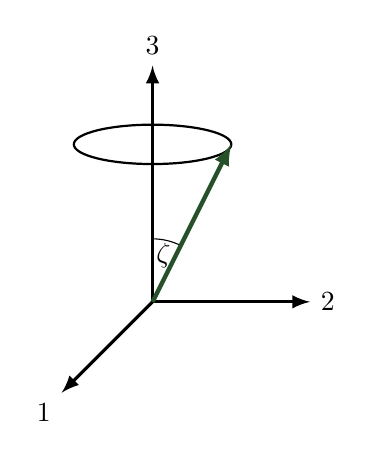
\begin{tikzpicture}
            \path (0, 1) coordinate (C) -- (0, 0) coordinate (B) -- (1, 2) coordinate (A) pic [draw, angle radius=0.8cm, "\(\zeta\)", angle eccentricity=0.75] {angle};
            \draw[very thick, ->] (0, 0, 0) -- (2, 0, 0) node[right] {2};
            \draw[very thick, ->] (0, 0, 0) -- (0, 3, 0) node[above] {3};
            \draw[very thick, ->] (0, 0, 0) -- (0, 0, 3) node[below left] {1};
            \draw[thick] (0, 2) circle [x radius = 1, y radius=0.25];
            \draw[highlight, ultra thick, ->] (0, 0) -- (1, 2);
        \end{tikzpicture}
        \caption[Symmetric top precession.]{A symmetric top rotating around its axis of symmetry will have an angular momentum, \(\vv{\omega}\), which precesses about the axis of symmetry tracing out a circle.}
        \label{fig:symmetric top precession}
    \end{figure}
    
    Since the motion is in a circle in the \((1,2)\)-plane the value of \(\omega_1^2 + \omega_2^2\) is constant, it's the radius of the circle squared.
    We also know that \(\omega_3\) is constant, and therefore \(\omega_3^2\) is constant.
    Combining these we see that \(\abs{\vv{\omega}} = \sqrt{\omega_1^2 + \omega_2^2 + \omega_3^2}\) is constant.
    The intrinsic angular momentum, \(\vv{J}\), then satisfies \(\vv{J}^2 = I_1^2A^2 + I_3^2\omega_3^2 = \text{constant}\), where \(A = \sqrt{\omega_1^2 + \omega_2^2}\) is the amplitude of the oscillations in the \(1\) and \(2\) directions, which is also the radius of the circle.
    We therefore also have \(\vv{J} \cdot \vv{\omega} = \text{constant}\).
    
    Since \(\vv{J}\cdot\vv{\omega}\), \(\vv{J}\cdot\ve{3}\), and \(\vv{\omega}\cdot\ve{3}\) are all constant \(\vv{J}\), \(\vv{\omega}\), and \(\ve{3}\) must make constant angles to each other.
    We can show that \((\vv{J} \times \vv{\omega}) \cdot \ve{3} = 0\), which shows that these three vectors are coplanar.
    This means that \(\vv{J}\) precesses along with \(\vv{\omega}\), since \(\ve{3}\) is fixed and \(\vv{J}\) must remain in the \(\ve{3}\)-\(\vv{\omega}\) plane.
    Therefore \(\vv{J}\) precesses with frequency \(\Omega\).
    
    Let \(\zeta\) be the angle between \(\ve{e}\) and \(\vv{\omega}\), and \(\tau\) be the angle between \(\ve{3}\) and \(\vv{J}\).
    Then
    \begin{equation}
        \cos \tau = \frac{\vv{J}\cdot\ve{3}}{\abs{\vv{J}}} = \frac{I_3\omega_3}{\sqrt{I_1^2A^2 + I_2^2\omega_3}} = \frac{\omega_3}{\sqrt{\frac{I_1^2}{I_3^2}A^2 + \omega_3^2}}.
    \end{equation}
    Similarly
    \begin{equation}
        \cos\zeta = \frac{\vv{\omega} \cdot \ve{3}}{\abs{\vv{\omega}}} = \frac{\omega_3}{\sqrt{A^2 + \omega_3^2}}.
    \end{equation}
    From this we see that if \(I_1 > I_3\), so \(I_1^2/I_3^2 \in (0, 1)\), then \(\cos\tau > \cos\zeta\), which means that \(\tau < \zeta\), since \(\cos\) is a decreasing function on \([0, \pi]\), which is also the total range of angles that \(\vv{J}\) and \(\vv{\omega}\) can make to \(\ve{3}\).
    The reverse, that if \(I_1 < I_3\), then \(\tau > \zeta\), also holds.
    
    For the special case where \(I_3 = I_1 = I_2\) Euler's equations reduce further to \(\dot{\vv{\omega}} = 0\), which is trivially true since \(\vv{J}\) and \(\vv{\omega}\) are parallel in this case.
    
    We wish to translate these results into the lab frame.
    The vectors \(\vv{J}\), \(\vv{\omega}\), and \(\ve{3}\) remain coplanar.
    The angular velocity, \(\vv{\omega}\), traces out a cone about \(\vv{J}\), called the space cone.
    We also know that \(\vv{\omega}\) traces out a body cone about \(\ve{3}\).
    We therefore find that the body cone rolls without slipping about the outside of the space cone if \(I_3 < I_1\), and inside the space cone if \(I_3 > I_1\).
    
    \section{Asymmetric Top}
    For the most general case in which all three principle moments of inertia are different the general solution to Euler's equations for torque free motion requires elliptic integrals and doesn't teach us much.
    Instead we will focus on looking for a solution where \(\vv{\omega}\) is constant in the body frame.
    From Euler's equations we see that this is only possible if two components of \(\vv{\omega}\) are zero in the body frame.
    Without loss of generality we take \(\omega_3\) to be the only non-zero component of \(\vv{\omega}\) and Euler's equations then give us
    \begin{align}
        I_1\dot{\omega}_1 &= (I_2 - I_3)\omega_2\omega_3 = 0,\\
        I_2\dot{\omega}_2 &= (I_3 - I_1)\omega_3\omega_1 = 0,\\
        I_3\dot{\omega}_3 &= (I_1 - I_2)\omega_1\omega_3 = 0.
    \end{align}
    So we see that as long as two components of \(\vv{\omega}\) are zero in the body frame then \(\vv{\omega}\) is constant.
    This means that
    \begin{important}
        an asymmetric body can only rotate with constant angular velocity if the rotation axis is one of the principal axes.
    \end{important}

    Suppose we have an asymmetric top rotating such that \(\vv{\omega} = \omega\ve{3}\) is constant.
    We can investigate the stability by seeing by considering \(\omega_1 = \varepsilon_1\), \(\omega_2 = \varepsilon_2\), and \(\omega_3 = \omega + \varepsilon_3\), where \(\varepsilon_i\) is small compared to \(\omega\).
    Inserting this in Euler's equations and expanding to first order in \(\varepsilon_i\) we get
    \begin{align}
        I_1\dot{\varepsilon}_1 &= (I_2 - I_3)(\omega + \varepsilon_3)\varepsilon_2 \approx (I_2 - I_3)\omega\varepsilon_2,\\
        I_2\dot{\varepsilon}_2 &= (I_3 - I_1)(\omega + \varepsilon_3)\varepsilon_1 \approx (I_3 - I_1)\omega\varepsilon_1,\\
        I_3\dot{\varepsilon}_3 &= (I_1 - I_2)\varepsilon_1\varepsilon_2 \approx 0.
    \end{align}
    Differentiating the first equation, remembering that \(I_i\) and \(\omega\) are constant, then substituting in the second equation we get
    \begin{equation}
        I_1\ddot{\varepsilon}_1 = (I_2 - I_3)\omega\dot{\varepsilon}_2 = (I_2 - I_3)\omega\frac{I_3 - I_1}{I_2}\omega\varepsilon_1,
    \end{equation}
    which we rearrange to get
    \begin{equation}
        I_1I_2\ddot{\varepsilon}_1 = (I_2 - I_3)(I_3 - I_1)\omega^2\varepsilon_1.
    \end{equation}
    If we swap the order of the two equations then we get the same equation but for \(\varepsilon_2\).
    
    The general solution to this equation is
    \begin{equation}
        \varepsilon_1 = A\e^{i\Omega t} + B\e^{-i\Omega t},
    \end{equation}
    and similar for \(\varepsilon_2\), where
    \begin{equation}
        \Omega^2 = \frac{(I_1 - I_3)(I_2 - I_3)}{I_1I_2}\omega^2.
    \end{equation}
    If \(I_3\) is either the smallest or largest moment of inertia then the right hand side is positive, meaning \(\Omega\) will be real.
    If \(I_3\) is the middle axis then \(\Omega\) is imaginary and hence \(\varepsilon_1\) grows exponentially as
    \begin{equation}
        \varepsilon_1 \sim B\e^{\abs{\Omega}t}.
    \end{equation}
    
    This results in the tennis racket theorem, so called because it is easy to demonstrate by throwing a tennis racket spinning about each of its three axes.
    \begin{thm}{Tennis Racket Theorem}{}
        Steady rotation about the intermediate axis is unstable, steady rotation about the major or minor axes is stable.
    \end{thm}
    
    \chapter{Lagrange's Method}
    Lagrange's method for rigid body motion is suitable for systems with a nonzero external torque.
    The trade-off with Euler's method is that Lagrange's method assumes that there is a point, \(O\), which is fixed.
    This point is normally not the centre of mass.
    We will consider the moment of inertia about \(O\), and call it \(I\) (we were calling the moment of inertia about a non-centre-of-mass point \(I'\) before).
    
    The angular momentum about \(O\) is
    \begin{equation}
        \vv{L} = I\vv{\omega}.
    \end{equation}
    The kinetic energy, including that due to the centre of mass motion, is
    \begin{equation}
        T = \frac{1}{2}\vv{\omega} \cdot I \vv{\omega} = \frac{1}{2}(I_1\omega_1^2 + I_2\omega_2^2 + I_3\omega_3^2)
    \end{equation}
    where \(I_i\) are the eigenvalues of \(I\), which we take to be arbitrary.
    
    We need a set of three generalised coordinates to specify the orientation of the body, fixing \(O\) fixes three of the six degrees of freedom.
    The canonical choice is to use \defineindex{Euler angles}, \((\vartheta, \varphi, \psi)\), which are defined by a series of rotations.
    There are multiple ways to define Euler angles which don't work together, we choose to use one convention, called the \(y\) convention, the only real advantage being that they are slightly more natural for the derivation of conservation laws.
    
    The process for defining Euler angles starts with the object in a reference state and then three rotations are made so that the object has the desired orientation, each rotation defining an angle:
    \begin{enumerate}
        \item Start with the object aligned with the body axes (those that rotate with the body) aligned with the space axes.
        \item Rotate the body in the \((x, z)\)-plane, the angle is \(\vartheta\).
        \item Rotate the body about the \(z\)-space-axis defining the angle \(\varphi\).
        \item Rotate the body about the \(3\)-axis (a body axis), defining the angle \(\psi\).
    \end{enumerate}
    These steps are drawn in \cref{fig:euler angles}.
    
    \begin{figure}
        \begin{subfigure}[b]{0.4\textwidth}
            \tikzsetnextfilename{euler-angle-1}
            \begin{tikzpicture}
                \draw[->, thick] (0, 0, 0) -- (3, 0, 0) node[right] {\(y\)};
                \draw[->, thick] (0, 0, 0) -- (0, 0, 3) node[below left] {\(x\)};
                \draw[->, thick] (0, 0, 0) -- (0, 3, 0) node[above] {\(z\)};
                \draw[->, highlight] (0, 0, 0) -- (2, 0, 0) node[below left] {\(2\)};
                \draw[->, highlight] (0, 0, 0) -- (0, 0, 2) node[above left] {\(1\)};
                \draw[->, highlight] (0, 0, 0) -- (0, 2, 0) node[below left] {\(3\)};
            \end{tikzpicture}
            \caption{Start with the body and space axes aligned.}
        \end{subfigure}
        \begin{subfigure}[b]{0.4\textwidth}
            \tikzsetnextfilename{euler-angle-2}
            \begin{tikzpicture}
                \draw[->, thick] (0, 0, 0) -- (3, 0, 0) node[right] {\(y\)};
                \draw[->, thick] (0, 0, 0) -- (0, 0, 3) node[below left] {\(x\)};
                \draw[->, thick] (0, 0, 0) -- (0, 3, 0) node[above] {\(z\)};
                \draw[->, highlight] (0, 0, 0) -- (2, 0, 0) node[below left] {\(2\)};
                \draw[->, highlight] (0, 0, 0) -- (0, -1.73205, 1) node[below left] {\(1\)};
                \draw[->, highlight] (0, 0, 0) -- (0, 1, 1.73205) node[above left] {\(3\)};
                \path[canvas is yz plane at x=0] (1, 0) coordinate (A) -- (0, 0) coordinate (B) -- ({cos(60)}, {sin(60)}) coordinate (C) pic [draw, "\(\vartheta\)", angle eccentricity = 0.7] {angle};
            \end{tikzpicture}
            \caption{Rotate through angle \(\vartheta\) about the \(y\)-axis.}
        \end{subfigure}
        \begin{subfigure}[b]{0.4\textwidth}
            \tikzsetnextfilename{euler-angle-3}
            \begin{tikzpicture}
                \draw[->, thick] (0, 0, 0) -- (3, 0, 0) node[right] {\(y\)};
                \draw[->, thick] (0, 0, 0) -- (0, 0, 3) node[below left] {\(x\)};
                \draw[->, thick] (0, 0, 0) -- (0, 3, 0) node[above] {\(z\)};
                \draw[->, highlight] (0, 0, 0) -- (1.73205, 1, 0) node[above right] {\(2\)};
                \draw[->, highlight] (0, 0, 0) -- (0.866025, -1.5, 1) node[below right] {\(1\)};
                \draw[->, highlight] (0, 0, 0) -- (-0.5, 0.866025, 1.73205) node[above left] {\(3\)};
                \path (1, 0) coordinate (A) -- (0, 0) coordinate (B) -- ({cos(30)}, {sin(30)}) coordinate (C) pic [draw, "\(\varphi\)", angle eccentricity = 1.3] {angle};
            \end{tikzpicture}
            \caption{Rotate through angle \(\varphi\) about the \(z\) axis.}
        \end{subfigure}
        \begin{subfigure}[b]{0.4\textwidth}
            \tikzsetnextfilename{euler-angle-4}
            \begin{tikzpicture}
                \draw[->, thick] (0, 0, 0) -- (3, 0, 0) node[right] {\(y\)};
                \draw[->, thick] (0, 0, 0) -- (0, 0, 3) node[below left] {\(x\)};
                \draw[->, thick] (0, 0, 0) -- (0, 3, 0) node[above] {\(z\)};
                \draw[->, highlight] (0, 0, 0) -- (1.06699, 1.61603, -0.5) node[above right] {\(2\)};
                \draw[->, highlight] (0, 0, 0) -- (1.61603, -0.799038, 0.866025) node[below right] {\(1\)} coordinate (C);
                \draw[->, highlight] (0, 0, 0) -- (-0.5, 0.866025, 1.73205) node[above left] {\(3\)};
                \draw[highlight, dashed] (0, 0, 0) -- (0.866025, -1.5, 1) coordinate (A);
                \path coordinate (B) pic [draw, "\(\psi\)", angle eccentricity = 1.35] {angle};
            \end{tikzpicture}
            \caption{Rotate through angle \(\psi\) about the \(3\)-axis.}
        \end{subfigure}
        \caption{How to define the rotation of a set of body axes relative to a set of space axes using Euler angles and the \(y\)-convention adopted in this course.}
        \label{fig:euler angles}
    \end{figure}
    
    \section{The Lagrangian}
    We want to find a Lagrangian, \(\lagrangian\), where the generalised coordinates are the Euler angles as defined in the previous section.
    The potential term is straight forward if we restrict ourselves to tops under gravity, the potential is simply
    \begin{equation}
        V = Mgl\cos\vartheta
    \end{equation}
    where \(l\) is the distance from the fixed point to the centre of mass and \(\vartheta\) is the Euler angle.
    
    The kinetic energy is not so straight forward.
    We know that in general
    \begin{equation}
        T = \frac{1}{2}\vv{\omega} \cdot I \vv{\omega} = \frac{1}{2}(I_1\omega_1^2 + I_2\omega_2^2 + I_3\omega_3^2).
    \end{equation}
    We therefore require \(\vv{\omega}\) as a function of \(\vartheta\), \(\varphi\), \(\psi\), \(\dot{\vartheta}\), \(\dot{\varphi}\), and \(\dot{\psi}\).
    
    Define the axes \(\ve{i}\) in the body frame as usual, and also an intermediate set of axes, \(\ve{i}'\), which are the axes after the second rotation, before the third rotation.
    Since the third rotation is about the \(3\)-axis we have that \(\ve{3} = \ve{3}'\).
    Looking down the \(3\)-axis we see that
    \begin{align}
        \ve{1} \cdot \ve{1}' &= \cos\psi,\\
        \ve{1} \cdot \ve{2}' &= \sin\psi,\\
        \ve{2} \cdot \ve{1}' &= -\sin\psi,\\
        \ve{2} \cdot \ve{2}' &= \cos\psi,
    \end{align}
    since this is simply a rotation in the plane normal to \(\ve{3}\) by angle \(\psi\).
    
    We will fist find the components of \(\vv{\omega}\) in the primed basis set.
    From the definition of the Euler angles we can identify that \(\dot{\vartheta}\) is the rate of rotation about the \(2'\)-axis, \(\dot{\varphi}\) is the rate of rotation about the \(z\)-axis, and \(\dot{\psi}\) is the rate of rotation about the \(3\)-axis.
    Therefore we have
    \begin{equation}
        \vv{\omega} = \dot{\vartheta}\ve{2}' + \dot{\varphi}\vh{z} + \dot{\psi}\ve{3}'.
    \end{equation}
    The \(2'\), \(3'\), and \(z\)-axes are not orthogonal, so this doesn't correspond directly to the components of \(\vv{\omega}\) in some orthonormal basis.
    We can decompose \(\vh{z}\) as
    \begin{equation}
        \vh{z} = (\vh{z} \cdot \ve{3}') \ve{3}' + (\vh{z} \cdot \ve{1}') \ve{1}' \ve{3}'\cos\vartheta - \ve{1}'\sin\vartheta.
    \end{equation}
    Doing so we get
    \begin{equation}
        \vv{\omega} = -\dot{\varphi} \sin\vartheta\ve{1}' + \dot{\vartheta}\ve{2}' + (\dot{\psi} + \dot{\varphi}\cos\vartheta)\ve{3}' = \sum_{i} \omega_i'\ve{i}'.
    \end{equation}
    
    Finally we can move to the unprimed basis using \(\ve{3}' = \ve{3}\) and hence \(\ve{3}' \cdot \ve{1} = \ve{3}' \cdot \ve{2} = 0\) so
    \begin{align}
        \omega_1 &= \ve{1} \cdot \vv{\omega} = -\dot{\varphi} \sin\vartheta \cos\psi + \dot{\vartheta} \sin\psi,\\
        \omega_2 &= \ve{2} \cdot \vv{\omega} = \hphantom{-}\dot{\varphi}\sin\vartheta\sin\psi + \dot{\vartheta\cos\varphi},\\
        \omega_3 &= \hphantom{-}\dot{\varphi}\cos\vartheta + \dot{\psi}.
    \end{align}
    This then gives the kinetic energy as
    \begin{align}
        T &= \frac{1}{2}(I_1\omega_1^2 + I_2\omega_2^2 + I_3\omega_3^2)\\
        &= \frac{1}{2}I_1(-\dot{\varphi}\sin\vartheta\cos\psi + \dot{\vartheta}\sin\psi)^2\\
        &+ \frac{1}{2}I_2(\dot{\varphi}\sin\vartheta\sin\psi + \dot{\vartheta}\cos\psi)^2\\
        &+ \frac{1}{2}I_3(\dot{\varphi}\cos\vartheta + \dot{\psi})^2.
    \end{align}
    Notice that this is quadratic in the velocities.
    
    This simplifies if the \(3\)-axis, which passes through the fixed pivot point, is also a symmetry axis of the body, which is to say that \(I_1 = I_3 = A\), denoting \(I_3 = C\) and expanding we then have
    \begin{align}
        T &= \frac{1}{2}[A(\omega_1^2 + \omega_2^2) + C\omega_3^2]\\
        &= \frac{1}{2}[A(\omega_1'^2 + \omega_2'^2) + C\omega_3^2]\\
        &= \frac{1}{2}[A(\dot{\vartheta}^2 + \dot{\varphi}^2\sin^2\vartheta) + C(\dot{\varphi}\cos\vartheta + \dot{\psi})].
    \end{align}
    Here we have used the fact that the \(1\) and \(2\) axes differ from the \(1'\) and \(2'\) axes by a rotation in the plane and therefore lengths are left unchanged, in particular \(\omega_1^2 + \omega_2^2 = \omega_1'^2 + \omega_2'^2\).
    This means that the final rotation was not necessary in this case.
    We could also have argued that the final result must be independent of \(\psi\) by symmetry in this case and then evaluated our earlier result for \(\psi = 0\) to achieve the same result.
    
    The Lagrangian is then
    \begin{equation}
        \lagrangian = \frac{1}{2}[A(\dot{\vartheta}^2 + \dot{\varphi}^2\sin^2\vartheta) + C(\dot{\varphi}\cos\vartheta + \dot\psi)^2] - Mgl\cos\vartheta.
    \end{equation}
    
    \section{Conservation Laws and Equations of Motion}
    Now that we have the Lagrangian we go through the usual procedure of deriving the conserved quantities and then the equations of motions.
    First we note that \(\lagrangian\) doesn't explicitly depend on \(\psi\), and so
    \begin{equation}
        p_\psi \coloneqq \diffp{\lagrangian}{\dot{\psi}} = C(\dot{\psi} + \dot{\varphi}\cos\vartheta) = I_3\omega_3
    \end{equation}
    is conserved.
    The reason for this conservation law is the symmetry of the system under rotations of the body about the 3-axis.
    Since the centre of mass is on the 3-axis the gravitational torque cannot change \(\omega_3\).
    By convention we define the conserved quantity
    \begin{equation}
        n = \omega_3 = \frac{p_\psi}{I_3} = \dot{\psi} + \dot{\varphi} \cos\vartheta
    \end{equation}
    which we call the \defineindex{spin}.
    
    The Lagrangian is also independent of \(\varphi\), and so
    \begin{equation}
        p_{\varphi} \coloneqq \diffp{\lagrangian}{\dot{\varphi}} = A\dot{\varphi}\sin^2\vartheta + C(\dot{\psi} + \dot{\varphi}\cos\vartheta)\cos\vartheta = A\dot{\varphi}\sin^2\vartheta + Cn\cos\vartheta
    \end{equation}
    is a conserved quantity.
    This corresponds to symmetry of the system under rotations about the \(z\)-axis.
    We can identify that \(p_\varphi = L_z\), is the \(z\) component of the orbital angular momentum.
    
    The Lagrangian \emph{does} depend explicitly on \(\vartheta\).
    The conjugate momentum is
    \begin{equation}
        p_{\vartheta} \coloneqq \diffp{\lagrangian}{\dot{\vartheta}} = A\dot{\vartheta}.
    \end{equation}
    The Euler--Lagrange equation for \(\vartheta\) is
    \begin{equation}
        \dot{p}_{\vartheta} = \diffp{\lagrangian}{\vartheta}
    \end{equation}
    which gives
    \begin{equation}
        A\ddot{\vartheta} = A\dot{\varphi}^2\sin\vartheta\cos\vartheta - C(\dot{\psi} + \dot{\varphi}\cos\vartheta)\dot{\varphi}\sin\vartheta + Mgl\sin\vartheta.
    \end{equation}
    This can be written as
    \begin{equation}
        A\ddot{\vartheta} = A\dot{\varphi}^2\sin\vartheta\cos\vartheta - Cn\dot{\varphi}\sin\vartheta + Mgl\sin\vartheta.
    \end{equation}
    
    The Lagrangian doesn't depend explicitly on time, hence the energy function,
    \begin{equation}
        h = \sum_{i=1}^{3}\dot{q_i}p_i - \lagrangian
    \end{equation}
    is conserved.
    Since the kinetic energy is quadratic in the velocity the value of the energy function coincides with the total energy \(E = T + V\).
    We can therefore compute \(T + V\) instead of \(h\) giving
    \begin{equation}
        E = \frac{A}{2}(\dot{\vartheta}^2 + \dot{\varphi}^2\sin^2\vartheta) + \frac{C}{2}n^2 + Mgl\cos\vartheta.
    \end{equation}
    We can write this as
    \begin{equation}
        \dot{\vartheta}^2 + \dot{\varphi}^2\sin^2\vartheta = \frac{2E - Cn^2}{A} - \frac{2Mgl\cos\vartheta}{A}.
    \end{equation}
    Substituting in the orbital angular momentum we can write this as
    \begin{equation}
        \dot{\vartheta}^2 = \frac{2E - Cn^2}{A} - \frac{2Mgl\cos\vartheta}{A} - \frac{(L_z - Cn\cos\vartheta)^2}{A^2\sin^2\vartheta}.
    \end{equation}
    
    After accounting for conservation laws we have only a single nontrivial degree of freedom, \(\vartheta\), described by a nonlinear first order ODE.
    
    \section{The Zone Function}
    Since \(\dot{\vartheta}\) must be real we require that \(\dot{\vartheta}^2 > 0\).
    For given value of \(n\), \(L_z\), and \(E\) this will define a zone of allowed values of the quantity \(u \coloneqq \cos\vartheta\).
    Writing \(\dot{u} = -\dot{\vartheta}\sin\vartheta\) we find that
    \begin{equation}
        \dot{u}^2 = \left( \frac{2E - Cn^2}{A} \right)(1 - u^2) - \frac{(L_z - Cnu)^2}{A^2} - \left( \frac{2Mgl}{A} \right) u(1 - u^2) = f(u).
    \end{equation}
    This is cubic in \(u\).
    We will therefore find an interval of values of \(u\) for which \(f(u)\) is positive and in which the initial value of \(f(u)\) lies.
    
    \section{Steady Precession}
    Conservation of energy gives us
    \begin{equation}
        \frac{1}{2}A\dot{\vartheta}^2 = E - \frac{Cn^2}{2} - Mgl\cos\vartheta - \frac{(L_z - Cn\cos\vartheta)^2}{2A\sin^2\vartheta} = E' - U(\vartheta).
    \end{equation}
    Here we have defined \(E' \coloneqq E - Cn^2/2\), and we define \(U(\vartheta)\) to account for the rest of the equation.
    We can identify this as the energy equation for a particle of \enquote{mass} \(A\) in a one dimensional potential, \(U(\vartheta)\), with total energy \(E'\).
    \(U(\vartheta)\) becomes very large as \(\vartheta\) tends to zero, and \(U(\vartheta)\) is bounded below.
    
    If \(\dot{\vartheta} = 0\) then we call this \defineindex{steady precession}.
    This occurs when
    \begin{equation}
        E' = \min U(L_z, n)
    \end{equation}
    and
    \begin{equation}
        \vartheta = \min \vartheta(L_z, n).
    \end{equation}
    We then have \(\vartheta = \text{constant}\) and since both \(L_z\) and \(n\) are conserved, and related to the degrees of freedom by
    \begin{equation}
        L_z = A\dot{\varphi}\sin^2\vartheta + Cn\cos\vartheta, \qqand n = \dot{\psi} + \dot{\varphi}\cos\vartheta.
    \end{equation}
    This means that both \(\dot{\psi}\) and \(\dot{\varphi}\) must also be constant.
    
    We find \(\vartheta_0 = \min \vartheta\) by finding where \(\diff{u}/{\vartheta} = 0\).
    This gives
    \begin{equation}
        \sin\vartheta_0 [\dot{\varphi}^2 A\cos\vartheta_0 - \dot{\varphi}Cn + Mgl] = 0.
    \end{equation}
    We can also find the same result from the Lagrange equation for \(\vartheta\) by noticing that \(\dot{\theta} = 0\) implies \(\ddot{\vartheta} = 0\).
    
    There are two solutions corresponding to two different physical actions:
    \begin{itemize}
        \item If \(\sin\vartheta_0 = 0\) then the top spins upright, we call this a \defineindex{sleeping top}.
        \item If \(\vartheta_0 \ne 0\), then the term in square brackets above must be zero, which we can solve to give
        \begin{equation}
            \dot{\varphi} = \frac{Cn \pm \sqrt{C^2n^2 - 4AMgl\cos\vartheta_0}}{2A\cos\vartheta_0}.
        \end{equation}
        If \(\cos\vartheta_0 > 0\), which corresponds to a top \emph{not} hanging below its pivot, so, for example, spinning on a table, then steady precession requires
        \begin{equation}
            C^2n^2 \ge 4AMgl\cos\vartheta_0.
        \end{equation}
        This gives a minimum speed for the top to be spinning to have steady precession.
    \end{itemize}
    
    \section{Fast Top}
    For a sufficiently fast spinning top we can expand the equation for \(\dot{\varphi}\) in steady state precession to give
    \begin{align}
        \dot{\varphi} &= \frac{Cn \pm (C^2n^2 - 4AMgl\cos\vartheta_0)^{1/2}}{2A\cos\vartheta_0}\\
        &\approx \frac{Cn}{2A\cos\vartheta_0} \left[ 1 \pm \left( 1 - \frac{2AMgl\cos\vartheta_0}{C^2n^2} \right) \right].
    \end{align}
    
    There are two possible roots to this equation:
    \begin{itemize}
        \item[\(-\)] Slow precession due to gravity, which has
        \begin{equation}
            \dot{\vartheta} = \frac{Mgl}{Cn}.
        \end{equation}
        \item[\(+\)] Free precession where
        \begin{equation}
            \dot{\varphi} = \frac{Cn}{A\cos\vartheta_0}.
        \end{equation}
    \end{itemize}
    
    These two limiting cases can also be checked by other methods.
    For example, for slow precession we can balance the gravitational torque such that\(\dot{\vv{L}}\) is constant.
    For free precession we can obtain the same result from Euler's equations of motion with zero torque.
    
    For a real gyroscope the free precession is damped by air resistance and the slow precession dominates.
    
    \section{Nutation}
    Keeping \(L_z\) fixed and increasing the energy, \(E'\), such that \(E'\) is slightly above \(\min U\) we get oscillations on top of the steady precession, we call this \defineindex{nutation}.
    The path traced by the \(3\)-axis will trace out either a wave or loops on the surface of a sphere while staying within a zone of values of \(\vartheta\).
    The path depends on the relative frequencies of the \(\varphi\) and \(\vartheta\) oscillations.
    For small amplitudes there is simple harmonic motion in \(\vartheta\) with frequency
    \begin{equation}
        \Omega_{\mathrm{nut}} = \sqrt{\frac{U''(\vartheta_0)}{A}}.
    \end{equation}
    
    For large enough spin,
    \begin{equation}
        Cn \gg \sqrt{4AMgl\cos\vartheta_0}
    \end{equation}
    we have \(\Omega_{\mathrm{nut}} \gg \dot{\varphi}\) and there are many oscillations per precession period.
    
    \section{Sleeping Top}
    The sleeping top is the case of \(\vartheta_0 = 0\).
    Lagrange's equation of motion is
    \begin{equation}
        A\ddot{\vartheta} = A\dot{\varphi}^2\sin\vartheta\cos\vartheta - Cn\dot{\varphi}\sin\vartheta + Mgl\sin\vartheta.
    \end{equation}
    Expanding this for small \(\vartheta\) we get
    \begin{equation}
        A\ddot{\vartheta} = (A\dot{\varphi}^2 - Cn\dot{\varphi} + Mgl)\vartheta.
    \end{equation}
    One solution to this is \(\vartheta = 0\).
    
    The top starts of upright and \(L_z = Cn\).
    Since both \(L_z\) and \(Cn\) are conserved this means that
    \begin{equation}
        Cn = L_z = A \dot{\varphi}\sin^2\vartheta + Cn\cos\vartheta.
    \end{equation}
    Expanding this for small \(\vartheta\) we get
    \begin{equation}
        \frac{1}{2}Cn\vartheta^2 = A\dot{\varphi}\vartheta^2.
    \end{equation}
    The sleeping top then has
    \begin{equation}
        \dot{\vartheta} = \frac{Cn}{2A}.
    \end{equation}
    This is the frequency at which a sleeping top precesses when perturbed by an infinitesimal distance from the vertical.
    We then have
    \begin{equation}
        A\ddot{\vartheta} = \left( Mgl - \frac{C^2n^2}{4A} \right)\vartheta.
    \end{equation}
    If \(n^2 > 4MglA/C^2\) then we have simple harmonic motion and the motion of the sleeping top is stable.
    If the spin is too low however then any perturbation will grow exponentially and so the top is unstable.
    
    We see this in real life when spinning a top.
    It will spin upright for a long time slowly decreasing in spin speed due to friction and at some point will rapidly start to veer away from upright before falling over.
    
    \part{Oscillations and Lagrange Multipliers}
    \chapter{Oscillations}
    \section{Static Equilibrium}
    Consider a system of \(D\) degrees of freedom in a time-independent conservative potential, that is
    \begin{equation}
        V = V(\{q\}, \nodependence{\{\dot{q}\}}, \nodependence{t}) = V(\{q\}), \qquad\text{with} \{q\} = (q_1, \dotsc, q_D).
    \end{equation}
    Static equilibrium, that is no motion, is only possible if all of the generalised forces, \(Q_i\), vanish together for some set of coordinates, \(\{q\}_{\mathrm{eq}}\).
    This set of coordinates defines an equilibrium position.
    
    We can redefine our coordinates, \(\{q\} \to \{q\} - \{q\}_{\mathrm{ed}}\), such that the equilibrium position is the origin.
    We then have
    \begin{equation}
        Q_j(\{0\}) = -\diffp{V(\{q\})}{q_j}[\{q\} = 0] = 0
    \end{equation}
    for all \(j\).
    Expanding \(V\) about this point terms linear in \(\{q\}\) vanish and we are left with
    \begin{equation}
        V(\{q\}) = V(\{0\}) + \frac{1}{2}\sum_i\sum_j \diffp{V}{q_i,q_j} q_iq_j + \order(\{q\}^3).
    \end{equation}
    The first term here is just a constant, which we will neglect.
    We then write
    \begin{equation}
        V(\{q\}) = \frac{1}{2}q_iV_{ij}q_j
    \end{equation}
    where we now use the summation convention and we define
    \begin{equation}
        V_{ij} \coloneqq \diffp{V}{q_i,q_j}[\{q\} = 0].
    \end{equation}
    This is a constant \(D \times D\) matrix of second derivatives evaluated at the origin.
    This matrix is symmetric (for sufficiently nice \(V\)).
    If \(\{q\} = 0\) is a local minimum then \(V_{ij}\) will be positive semi-definite, that is the eigenvalues will all be nonnegative, this ensures that we cannot decrease the potential energy by changing the value of any of \(\{q\}\), and hence it is indeed a minimum.
    
    \section{The Lagrangian}
    We will consider only systems where the kinetic energy is time independent and quadratic in the velocities.
    We then have
    \begin{equation}
        T = T(\{q\}, \{\dot{q}\}, \nodependence{t}) = \frac{1}{2}\dot{q}_iT_{ij}\dot{q}_j.
    \end{equation}
    Here \(T_{ij}\) is a matrix depending, in general, on the coordinates, \(\{q\}\).
    
    For small displacements about the equilibrium we can take \(T_{ij}\) to be an approximately constant matrix.
    It is convenient to choose \(T_{ij}\) to be symmetric.
    This is possible since we can always symmetrise any asymmetric matrix, \(\tilde{T}_{ij}\), by writing \((\tilde{T}_{ij} + \tilde{T}_{ji})/2\), without changing the value of \(T\).
    Kinetic energies are typically positive and so \(T_{ij}\) is positive definite, that is all its eigenvalues are positive.
    
    For small displacements the Lagrangian is
    \begin{equation}
        \lagrangian = T - V = \frac{1}{2}(\dot{q}_iT_{ij}\dot{q}_j - q_iV_{ij}q_j).
    \end{equation}
    Lagrange's equations then give
    \begin{equation}
        \diff*{\left( \diffp{\lagrangian}{\dot{q}_i} \right)}{t} = \diffp{\lagrangian}{q_i} \implies T_{ij}\ddot{q}_j = -V_{ij}q_j.
    \end{equation}
    These are linear equations, so we say that the system has been linearised by the assumption that the displacements are small.
    We can then solve the resulting equations with matrix methods.
    
    We define \define{normal modes}\index{normal mode} to be the solutions to he equations of motion in which the generalised coordinates all oscillate with the same angular frequency, \(\omega\):
    \begin{equation}
        q_j = a_j\cos(\omega t + \varepsilon_j).
    \end{equation}
    The equation of motion is then
    \begin{equation}
        \omega^2T_{ij}a_j + V_{ij}a_j = 0.
    \end{equation}
    Setting \(\lambda \coloneqq \omega^2\) we get
    \begin{equation}
        (V_{ij} - \lambda T_{ij})a_j = 0.
    \end{equation}
    This is a sort of generalised eigenvalue equation, the basic version being \((M_{ij} - \lambda\delta_{ij})a_j = 0\).
    The process of solving this equation is very similar to the eigenvalue equation:
    \begin{enumerate}
        \item Find the eigenvalues, \(\lambda^{(i)}\), by solving
        \begin{equation}
            \det(V - \lambda T) = 0.
        \end{equation}
        \item For a given \(\lambda^{(k)}\) write
        \begin{equation}
            (V_{ij} - \lambda^{(k)}T_{ij})e_j^{(k)} = 0.
        \end{equation}
        This defines an (unnormalised) eigenvector, \(\vv{e^{(k)}}\), for the \(k\)th mode which has \(j\)th component \(e_j^{(k)}\).
        In general these eigenvectors will not be orthogonal.
    \end{enumerate}
    
    \section{Triatomic Molecule}
    Consider a triatomic molecule, such as \ce{H2O} or \ce{CO2}, with one central atom of mass \(M\) and two outer atoms of mass \(m\).
    We can model the bonds as being springs with spring constant \(K\).
    See \cref{fig:triatomic molecule}.
    
    \begin{figure}
        \tikzsetnextfilename{triatomic-molecule}
        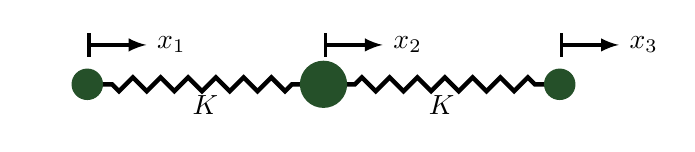
\begin{tikzpicture}
            \tikzset{spring/.style = {ultra thick, decoration={zigzag, pre length=0.4cm, post length=0.25cm}, decorate}}
            \draw[spring] (0, 0) -- (3, 0) node[midway, below] {\(K\)};
            \draw[spring] (0, 0) -- (-3, 0) node[midway, below] {\(K\)};
            \fill[highlight] (0, 0) circle [radius = 0.3];
            \fill[highlight] (3, 0) circle [radius = 0.2];
            \fill[highlight] (-3, 0) circle [radius = 0.2];
            \foreach \x in {-3, 0, 3} {
                \pgfmathsetmacro{\i}{int((\x + 6)/3)}
                \draw[very thick, |->] (\x, 0.5) -- (\x + 0.75, 0.5) node[right] {\(x_\i\)};
            }
            \draw[white] (-3.75, 0) -- (-3.75, 0);
        \end{tikzpicture}
        \caption{Triatomic molecule.}
        \label{fig:triatomic molecule}
    \end{figure}
    
    We define the coordinates \(x_i\) as the displacements of the atoms, as shown in \cref{fig:triatomic molecule}.
    The kinetic energy is then
    \begin{equation}
        T = \frac{1}{2}m(\dot{x}_1^2 + \dot{x}_3^2) + \frac{1}{2}M\dot{x}_2^2.
    \end{equation}
    The potential is simply the energy stored in the springs, which is related to the extension of the sprints, \(x_1 - x_2\) and \(x_3 - x_2\):
    \begin{equation}
        V = \frac{1}{2}K(x_1 - x_2)^2 + \frac{1}{2}K(x_3 - x_2)^2 = \frac{1}{2}K(x_1^2 + 2x_2^2 + x_3^2 - 2x_1x_2 - 2x_3x_2).
    \end{equation}
    Choosing \(x_i\) as our generalised coordinates we find the matrices for \(T\) and \(V\) are
    \begin{equation}
        T_{ij} = 
        \begin{pmatrix}
            m & 0 & 0\\
            0 & M & 0\\
            0 & 0 & m
        \end{pmatrix}
        , \qqand V_{ij} = 
        \begin{pmatrix}
            K & -K & 0\\
            -K & 2K & -K\\
            0 & -K & K
        \end{pmatrix}
        .
    \end{equation}
    Note that we have chosen \(V_{ij}\) to be symmetric, there are other nonsymmetric matrices that would give the same result, for example
    \begin{equation}
        \begin{pmatrix}
            K & -2K & 0\\
            0 & 2K & 0\\
            0 & -2K & K
        \end{pmatrix}
        .
    \end{equation}
    The generalised eigenvalue problem is then to solve
    \begin{equation}
        \begin{vmatrix}
            K - \lambda m & -K + 7\\
            -K & 2K - \lambda M & -K\\
            0 & -K & K - \lambda m
        \end{vmatrix}
        = 0.
    \end{equation}
    This gives us the characteristic polynomial
    \begin{equation}
        \lambda(K - \lambda m)(\lambda mM - (M + 2m)K) = 0.
    \end{equation}
    This has roots
    \begin{equation}
        \lambda^{(1)} = 0, \qquad \lambda^{(2)} = \frac{K}{m}, \qqand \lambda^{(3)} = \frac{K(2m + M)}{Mm}.
    \end{equation}
    To find the eigenvectors, \(\vv{e^{(k)}}\) we solve
    \begin{equation}
        (V_{ij} - \lambda^{(k)}T_{ij})e_j^{(k)} = 0.
    \end{equation}
    We find that
    \begin{equation}
        \vv{e^{(1)}} = (1, 1, 1), \qquad \vv{e^{(2)}} = (1, 0, -1), \qqand \vv{e^{(3)}} = (1, -2m/M, 1).
    \end{equation}
    Writing \(\omega_i = \sqrt{\lambda^{(i)}}\) we can interpret these three eigenvectors as describing three linearly independent modes of vibration:
    \begin{enumerate}
        \item The first is uniform motion of the whole molecule, all three atoms move the same amount and the oscillation frequency is \(\omega_1 = 0\), since there is no restoring force as the molecule is free to move.
        \item The second is oscillation at frequency \(\omega_2 = \sqrt{K/m}\), which corresponds to the two outer atoms moving \(\pi\) out of phase with the middle atom stationary.
        \item The third is oscillation at frequency \(\omega_3 = \sqrt{K(2m + M)/(mM)}\), which corresponds to the two outer atoms moving in the same direction and the central atom moving in the opposite direction.
    \end{enumerate}
        
    The general solution describing the motion is then a linear combination of these three distinct types of motion:
    \begin{equation}
        \vv{x}(t) = A_1 \vv{e^{(1)}}\cos(\omega_1t + \varphi_1) + A_2\vv{e^{(2)}}\cos(\omega_2 t + \varphi_2) + A_3 \vv{e^{(3)}} \cos(\omega_3 t + \varphi_3).
    \end{equation}
    The amplitudes, \(A_i\), and phases, \(\varphi_i\), are set by the initial conditions, giving 6 constants having solved 3 second order differential equations.
    
    In this case since \(\omega_1 = 0\) the cosine factor is just a constant.
    In addition \(A_1\) can be arbitrarily large.
    Taking a limit we find that
    \begin{equation}
        \lim_{\omega_1 \to 0} A_1\cos(\omega_1 t + \varphi_1) = A + vt
    \end{equation}
    for some constants \(A\) and \(v\).
    This means we should really write the solution as
    \begin{equation}
        \vv{x}(t) = (A + vt) \vv{e^{(1)}} + A_2\vv{e^{(2)}}\cos(\omega_2 t + \varphi_2) + A_3 \vv{e^{(3)}} \cos(\omega_3 t + \varphi_3).
    \end{equation}
    To avoid this we usually neglect zero modes where the whole system moves together by simply restricting \(V_{ij}\) to be positive definite and treat the motion of the whole system separately.
    
    \section{Simultaneous Diagonalisation}
    The matrix \(T\) is positive definite.
    We will show that there is a coordinate transformation such that in the transformed coordinates both \(T\) and \(V\), which are symmetric, are simultaneously diagonalised.
    We start by applying an orthogonal transformation, \(C\), to \(T\) and \(V\) such that \(T\) is diagonalised, defining
    \begin{equation}
        T' \coloneqq C^{\trans}TC, \qqand V' \coloneqq C^{\trans}VC.
    \end{equation}
    This is always possible since \(T\) is symmetric.
    We now have
    \begin{equation}
        T' = 
        \begin{pmatrix}
            T_1 &     &        & \\
                & T_2 &        & \\
                &     & \ddots & \\
                &     &        & T_D
        \end{pmatrix}
    \end{equation}
    Since \(T\) is positive definite and \(T_i\) are the eigenvalues of \(T\) all of \(T_i\) are positive, and hence \(\sqrt{T_i}\) are real.
    This means we can define the real matrix
    \begin{equation}
        K \coloneqq 
        \begin{pmatrix}
            1/\sqrt{T_1} &              &        & \\
                         & 1/\sqrt{T_2} &        & \\
                         &              & \ddots & \\
                         &              &        & 1/\sqrt{T_D}
        \end{pmatrix}
    \end{equation}
    We can then apply a transform with this matrix defining
    \begin{equation}
        T'' = K^\trans C^\trans TCK, \qqand V'' = K^{\trans}C^{\trans}VCK.
    \end{equation}
    The way we have defined \(K\) means that \(T'' = K^{\trans}T'K = KT'K = \ident\).
    Also \(V''\) is still symmetric.
    
    We then apply a final orthogonal transformation, \(D\), to diagonalise \(V''\), which is possible since it is symmetric.
    This has no effect on \(T''\) since \(T'' = \ident\) so \(D^{\trans}T''D = D^{\trans}\ident D = D^{\trans}D = D^{-1}D = \ident\), since \(D\) is orthogonal.
    We therefore define \(T''' = DT''D = \ident\) and \(V''' = D^{\trans}V''D\) which gives a diagonal \(V'''\):
    \begin{equation}
        V''' =
        \begin{pmatrix}
            \lambda_1 &           &        & \\
                      & \lambda_2 &        & \\
                      &           & \ddots & \\
                      &           &        & \lambda_D
        \end{pmatrix}
        .
    \end{equation}
    Defining \(M \coloneqq CKD\) we have
    \begin{equation}
        T''' = M^{\trans}TM = \ident, \qqand V''' = M^{\trans}VM.
    \end{equation}
    We can now interpret this as a coordinate transformation:
    \begin{equation}
        q_i \to \tilde{q}_i, \qquad\text{with}\qquad q_i = M_{ij}\tilde{q}_j.
    \end{equation}
    This is invertible and so \(\{\tilde{q}\}\) are a valid set of generalised coordinates.
    In general this is \emph{not} an orthogonal transformation, unless \(T_i = 1\) for all \(i\).
    
    Dropping the tilde and working exclusively in this simultaneously diagonalised basis we have \(T_{ij} = \delta_{ij}\) and \(V_{ij} = \lambda_i\delta_{ij}\).
    The Lagrangian is then
    \begin{equation}
        \lagrangian = \frac{1}{2}\dot{q}_iT_{ij}\dot{q}_j - \frac{1}{2}q_iV_{ij}q_j = \sum_{i} \left[ \frac{1}{2}\dot{q}_i^2 - \frac{1}{2}\lambda_iq_i^2 \right].
    \end{equation}
    We now stop using the summation convention.
    This form of the Lagrangian is called the \define{normal form}\index{normal!form} and the transformed coordinates the \define{normal coordinates}\index{normal!coordinates}.
    The Euler--Lagrange equations are now very simple:
    \begin{equation}
        \ddot{q}_i = -\lambda_iq_i.
    \end{equation}
    Which is simple harmonic motion with the general solution
    \begin{equation}
        q_i(t) = A_i\cos(\omega_i t + \varphi_i).
    \end{equation}
    Where as usual \(\omega_i = \sqrt{\lambda_i}\), and \(A_i\) and \(\varphi_i\) are constants of integration fixed by the initial conditions.
    
    We don't need to sum over all of the modes any more.
    Each coordinate executes simple harmonic motion independent of the other coordinates.
    The effort in solving the motion is moved to finding the transformation that diagonalises both matrices simultaneously which allows us to relate the transformed coordinates, which may not have an obvious physical meaning, to a set of more easily understandable generalised coordinates.
    
    When solving problems with this method we don't typically find the matrices \(C\), \(K\), and \(D\) separately, instead we identify that \(M_{ij} = e_i^{(j)}\).
    This shows that the two methods of solving the equations are almost identical since both involve solving the generalised eigenvalue equation \((V_{ij} - \lambda T_{ij})a_j = 0\), and finding the eigenvectors, \(\vv{e^{(k)}}\).
    The only difference is in how we separate out the individual components of the motion.
    
    \chapter{Lagrange Multipliers}
    Recall that a holonomic constraint is one which can be written in the form \(f(\{q\}, t) = 0\).
    So far we have been accounting for these by using them to reduce the number of degrees of freedom, and hence the number of generalised coordinates in a problem.
    There is another method in which we can include them directly in the Lagrangian.
    This is the method of Lagrange multipliers.
    This method can also be used in many other optimisation procedures involving minimisation of functionals.
    
    Consider a system of two coordinates, \(x\) and \(y\), which are related by the holonomic constraint \(f(x, y) = 0\) for some function \(f\).
    We construct the Lagrangian, \(\lagrangian = T - V\), as normal using both coordinates treating them as independent.
    We find that the change in action for a change in the coordinates, \(x \to x + \delta x\) and \(y \to y + \delta y\) is
    \begin{equation}
        \delta S = \int \left( \diff*{\left( \diffp{\lagrangian}{\dot{x}} \right)}{t} - \diffp{\lagrangian}{x} \right)\delta x + \left( \diff*{\left( \diffp{\lagrangian}{\dot{y}} \right)}{t} - \diffp{\lagrangian}{y} \right)\delta y \dd{t}.
    \end{equation}
    If \(x\) and \(y\) are independent coordinates then both brackets would have to vanish independently.
    However, we are assuming that they aren't independent.
    
    Now consider the Lagrangian
    \begin{equation}
        \lagrangian'(x, y, t) = \lagrangian(x, y) + \lambda f(x, y).
    \end{equation}
    Note that this has the same numeric value, since \(f(x, y) = 0\), but the functional form is different, which we know can be important for functional calculus.
    The change in the action can then be written as
    \begin{equation}
        \delta S' = \int \left( \diff*{\left( \diffp{\lagrangian}{\dot{x}} \right)}{t} - \diffp{\lagrangian}{x} + \lambda\diffp{f}{x} \right)\delta x + \left( \diff*{\left( \diffp{\lagrangian}{\dot{y}} \right)}{t} - \diffp{\lagrangian}{y} + \lambda\diffp{f}{y} \right).
    \end{equation}
    Since \(\lambda\) is arbitrary we can choose it such that each term must be zero.
    
    In general if we have \(n\) (not necessarily independent) coordinates and \(m\) constraints, of the form
    \begin{equation}
        f_\alpha(q_1, \dotsc, q_n, t) = 0
    \end{equation}
    for \(\alpha = 1, \dotsc, m\), then we define the modified Lagrangian
    \begin{equation}
        \lagrangian'(q_1, \dotsc, q_n, \lambda_1, \dotsc, \lambda_m) = \lagrangian(q_1, \dotsc, q_n) + \sum_{\alpha} \lambda_\alpha f_\alpha(q_1, \dotsc, q_n, t).
    \end{equation}
    We then take all of \(q_i\) and \(\lambda_\alpha\) as our coordinates and form the Euler--Lagrange equations for them.
    Since there is no \(\dot{\lambda}_\alpha\) dependence in \(\lagrangian'\) the Euler--Lagrange equations for \(\lambda_\alpha\) immediately return the constraint \(f_{\alpha}(\{q\}) = 0\).
    
    \section{Holonomic Example}
    Consider Atwood's machine from \cref{sec:atwood's machine}.
    Previously we treated the constraint by reducing the number of degrees of freedom.
    Now we shall do so with Lagrange multipliers.
    Using the notation of \cref{sec:atwood's machine} we know that the kinetic energy and potential are
    \begin{equation}
        T = \frac{1}{2}M\dot{x}^2 + \frac{1}{2}m\dot{y}^2, \qqand V = Mgx + mgy.
    \end{equation}
    Our holonomic constraint is \(x + y + \ell = 2h\), which when written in the required form is \(f(x, y) = x + y + \ell - 2h = 0\).
    
    The Lagrangian accounting for this constraint is
    \begin{equation}
        \lagrangian = \frac{1}{2}M\dot{x}^2 + \frac{1}{2}m\dot{y}^2 - Mgx - mgy + \lambda(x + y + \ell - 2h).
    \end{equation}
    We then take \(x\), \(y\), and \(\lambda\) as our coordinates.
    The Euler--Lagrange equations are then
    \begin{align}
        \diff*{\left( \diffp{\lagrangian}{\dot{x}} \right)}{t} &= \diff*{(M\dot{x})}{t} = M\ddot{x} = \diffp{\lagrangian}{x} = -Mg + \lambda,\\
        \diff*{\left( \diffp{\lagrangian}{\dot{y}} \right)}{t} &= \diff*{(m\dot{y})}{t} = m\ddot{x} = \diffp{\lagrangian}{y} = -mg + \lambda,\\
        \diff*{\left( \diffp{\lagrangian}{\dot{\lambda}} \right)}{t} = 0 = \diffp{\lagrangian}{\lambda} = x + y + \ell - 2h.
    \end{align}
    Notice that we cannot drop the constant terms in order for this method to work, since we need them to ensure that we get the full constraint back.
    Differentiating the last of these equations twice, which is just the constraint, we get \(\ddot{x} = -\ddot{y}\).
    We can subtract the second from the first to eliminate \(\lambda\) giving
    \begin{equation}
        M\ddot{x} + Mg = -m\ddot{x} + mg.
    \end{equation}
    This gives the result
    \begin{equation}
        \ddot{x} = -\frac{(M - m)g}{M + m}.
    \end{equation}
    This is the same solution we found using the other method.
    
    Notice that if we missed the constraint we would have found \(\ddot{x} = \ddot{y} = -g\), which corresponds to both masses being free.
    This pattern, of missing constraints giving the free case, is fairly common.
    
    \section{Non-Holonomic Example}
    Consider a hanging chain of length \(\ell\) and density \(\rho\) hanging between two points which are the same height and are a distance \(2a\) apart, with \(2a < D\), the length of the chain.
    The chain will hang in the shape which minimises the potential energy, which is the same as maximising the action, since we are looking for a stationary solution so the kinetic energy is zero.
    
    The total energy is given by integrating along the chain:
    \begin{equation}
        V = \rho g\int y \dd{s} = \rho g \int_{-a}^{a} y\sqrt{1 + y'^2} \dd{x}.
    \end{equation}
    Here we take \(x = 0\) as the midpoint between the two attachment points.
    
    The constraint that we need to introduce is the constant length of the chain.
    This can be written in integral form as
    \begin{equation}
        \int \dl{s} = \int \sqrt{1 + y'^2} \dd{x} = D
    \end{equation}
    This gives us the functional
    \begin{equation}
        I = \int_{-a}^{a} \left[ \rho gy\sqrt{1 + y'^2} + \lambda\left( \sqrt{1 + y'^2} - D \right) \right] \dd{x}.
    \end{equation}
    
    Since there is no explicit dependence on \(x\) we know that the following is constant:
    \begin{equation}
        y' \diffp{F}{y'} - F = -\frac{\rho gy + \lambda}{\sqrt{1 + y'^2}} = C.
    \end{equation}
    The solution to this is
    \begin{equation}
        y(x) = \frac{C}{\rho g} \cosh\left( \frac{\rho g x}{C} \right) - \frac{\lambda}{\rho g}.
    \end{equation}
    Requiring \(y(\pm a) = 0\) we get
    \begin{equation}
        \lambda = C \cosh\left( \frac{\rho g a}{C} \right).
    \end{equation}
    We then find \(C\) by requiring that the total length be \(D\), which gives
    \begin{equation}
        D = \int_{-a}^{a}\sqrt{1 + y'^2} \dd{x} = \int_{-a}^{a} \cosh\left( \frac{\rho g x}{C} \right) \dd{x},
    \end{equation}
    here we have used
    \begin{equation}
        \diff*{\cosh x}{x} = \sinh x, \qqand 1 + \sinh^2 x = \cosh^2 x.
    \end{equation}
    
    %Appendicies
    \appendixpage
    \begin{appendices}
        \chapter{Differential Equations}
Many of the equations of motion we will derive are second order linear ordinary differential equations of the form
\begin{equation}
    ay''(x) + by'(x) + cy(x) = f(x)
\end{equation}
for some constants \(a\), \(b\), and \(c\), and functions \(y\) and \(f\).
There is a general procedure for solving such equations.
\begin{enumerate}
    \item First define the homogenous equation
    \begin{equation}
        ay''(x) + by'(x) + cy(x) = 0.
    \end{equation}
    This is important since if \(y_1\) is a solution to the homogeneous equation and \(y_p\) is a solution to the inhomogeneous equation then \(y_p + \lambda y_1\) with \(\lambda\) being a constant, is a solution to the original inhomogeneous equation also.
    The most general solution is the solution to the inhomogeneous equation and a linear combination of solutions to the homogenous equation.
    The number of solutions to the homogenous equation is equal to the order of the equation, so for our purposes 2.
    \item Solve the homogenous equation.
    This is usually done by making a guess and substituting into the homogenous equation and solving for any unknowns in the guess.
    The most common guess is of the form \(\e^{mx}\).
    If we make this guess after substitution we have
    \begin{equation}
        (am^2 + bm + c)\e^{mx} = 0.
    \end{equation}
    Since \(\e^{mx} \ne 0\) we must therefore have that the quadratic in \(m\) is zero.
    This gives us two values for \(m\), \(m_1\) and \(m_2\).
    If \(m_1 \ne m_2\) then we define
    \begin{equation}
        y_1(x) = \e^{m_1x}, \qqand y_2(x) = \e^{m_2x}.
    \end{equation}
    If \(m_1 = m_2\) then instead define
    \begin{equation}
        y_1(x) = \e^{m_1x}, \qqand y_2(x) = x\e^{m_1x}.
    \end{equation}
    Occasionally other guesses, such as trig functions, make more sense, particularly if there are no first derivatives in the equation.
    
    \item Returning to the inhomogeneous equation we now need to find a solution, \(y_p\), of course if the original equation was inhomogeneous then this step can be skipped.
    We again do this by guessing.
    The exact guess depends on the form of \(f\) but some common choices are given in \cref{tab:common guesses for differential equation}.
    \begin{table}
        \caption{Common guesses to solve the inhomogeneous differential equation \(ay''(x) + by'(x) + cy(x) = f(x)\) for different functions \(f\).}
        \label{tab:common guesses for differential equation}
        \begin{tabular}{cc}
            \toprule
            Form of \(f\) & Suggestion for \(y_p\)\\\midrule
            Constant, \(k\) & Constant \(k/c\)\\
            Polynomial in \(x\) & Polynomial in \(x\)\\
            \(ke^{\alpha x}\) & \(A e^{\alpha x}\)\\
            \(\sin(\alpha x)\) and/or \(\cos(\alpha x)\) & \(A\sin(\alpha x) + B\cos(\alpha x)\)\\\bottomrule
        \end{tabular}
    \end{table}
    Once you have chosen a function substitute it in and see if it is valid.
    
    \item If you have no boundary conditions then you are done.
    The solution is
    \begin{equation}
        y(x) = y_p(x) + \sum_i\lambda_i y_i(x)
    \end{equation}
    where \(y_i\) are solutions to the homogeneous equation.
    If you have boundary conditions then substitute them into this equation and solve for \(\lambda_i\).
\end{enumerate}

\begin{exm}{}{}
    Suppose we wish to solve
    \begin{equation}
        y''(x) + 4y'(x) + 4y(x) = \sin(3x),
    \end{equation}
    with the boundary conditions \(y(0) = 10\) and \(y'(0) = 0\).
    
    We start by defining the homogeneous equation
    \begin{equation}
        y''(x) + 4y'(x) + 4y(x) = 0.
    \end{equation}
    We propose that \(\e^{mx}\) is a solution to this.
    Substituting this in we find
    \begin{equation}
        (m^2 + 4m^2 + 4)\e^{mx} = 0.
    \end{equation}
    The quadratic has one repeated root \(m = -2\) and so our solutions to the homogenous equation are
    \begin{equation}
        y_1(x) = \e^{-2x}, \qqand y_2(x) = x\e^{-2x}.
    \end{equation}
    
    In this case \(f(x) = \sin(3x)\) and so we try a solution of the form
    \begin{equation}
        y_p(x) = A\sin(3x) + B\cos(3x).
    \end{equation}
    Substituting this into our original equation we have
    \begin{multline}
        -9A\sin(3x) -9B\cos(3x) + 12A\cos(3x) - 12B\sin(3x)\\ + 4A\sin(3x) + 4B\cos(3x)\\= -(5A + 12B)\sin(3x) + (12A - 5B)\cos(3x).
    \end{multline}
    In order for this to be equal to \(\sin(3x)\) we require that
    \begin{equation}
        5A + 12B = -1, \qqand 12A - 5B = 0.
    \end{equation}
    Solving these simultaneous equations gives us
    \begin{equation}
        A = -\frac{5}{169}, \qqand B = -\frac{12}{169}.
    \end{equation}
    Hence our solution is
    \begin{equation}
        y_p(x) = -\frac{5}{169} \sin(3x) - \frac{12}{169} \cos(3x).
    \end{equation}
    
    The general solution is then
    \begin{equation}
        y(x) = -\frac{5}{169} \sin(3x) - \frac{12}{169} \cos(3x) + \lambda_1\e^{-2x} + \lambda_2x\e^{-2x}.
    \end{equation}
    Substituting for our first initial condition, \(y(0) = 10\), we have
    \begin{equation}
        y(0) = -\frac{12}{169} + \lambda_1 = 10 \implies \lambda_1 = \frac{1702}{169}.
    \end{equation}
    The second initial condition, \(y'(0) = 0\), gives us
    \begin{equation}
        y'(0) = -\frac{15}{169} - 2\frac{1702}{169} - 2\lambda_2 = 0 \implies \lambda_2 = -\frac{263}{26}.
    \end{equation}
    Hence our final solution is
    \begin{equation}
        y(x) = -\frac{5}{169} \sin(3x) - \frac{12}{169} \cos(3x) + \frac{1702}{169}\e^{-2x} - \frac{263}{26}x\e^{-2x}.
    \end{equation}
\end{exm}

        \chapter{Electromagnetism}\label{sec:electromagnetism}
        \begin{rmk}
            For more details see the notes for electromagnetism.
        \end{rmk}
        \section{Maxwell's Equations}
        Maxwell's equations are, in SI units
        \begin{align}
            \div \vv{E} &= \frac{\rho}{\varepsilon_0}, \tag{M1}\\
            \div \vv{B} &= 0, \tag{M2}\\
            \curl \vv{E} &= -\diffp{\vv{B}}{t}, \tag{M3}\\
            \curl \vv{B} &= \mu_0\left( \vv{j} + \varepsilon_0\diffp{\vv{E}}{t} \right). \tag{M4}
        \end{align}
        Here \(\vv{E}\) and \(\vv{B}\) are the electric and magnetic fields, \(\rho\) is the electric charge density, \(\vv{j}\) is the electric current density, \(\varepsilon_0\) and \(\mu_0\) are the permittivity and permeability of free space, also known as the electric and magnetic constants.
        The value of \(\varepsilon_0\) and \(\mu_0\), and the speed of light, \(c = 1/\sqrt{\varepsilon_0\mu_0}\), determine the system of units used to measure \(\vv{E}\), \(\vv{B}\), \(\rho\), and \(\vv{j}\).
        
        The force on a particle of charge \(e\) in an electromagnetic filed is given by
        \begin{equation}
            \vv{F} = e(\vv{E} + \dot{\vv{r}}\times\vv{B})
        \end{equation}
        where \(\vv{r}\) is the position of the particle.
        This force is velocity dependent, and therefore cannot be treated with a simple \(T - V\) Lagrangian (unless \(\vv{B} = \vv{0}\)).
        
        \section{Potentials}
        It is a well known fact of vector calculus that a divergence free vector field, such as \(\vv{B}\), can be written as the curl of a vector field:
        \begin{equation}
            \div \vv{B} = 0 \iff \exists \vv{A} \text{ such that } \vv{B} = \curl \vv{A}.
        \end{equation}
        In the case of \(\vv{B}\) being the magnetic field we call \(\vv{A}\) the magnetic vector potential.
        
        Writing M3 in terms of the vector potential we have
        \begin{equation}\label{eqn:derivation of electric potential}
            \curl \vv{E} = -\diffp*{(\curl\vv{A})}{t} \implies \curl \left( \vv{E} + \diffp{\vv{A}}{t} \right) = 0.
        \end{equation}
        A standard result of vector calculus is that any curl free field, \(\vv{G}\), such that \(\curl\vv{G} = 0\), can be written as the gradient of a scalar potential, \(\varphi\):
        \begin{equation}
            \curl \vv{G} = 0 \iff \exists \varphi \text{ such that } \vv{G} = -\grad\varphi
        \end{equation}
        where the negative sign is a convention.
        From \cref{eqn:derivation of electric potential} we see that
        \begin{equation}
            \vv{E} + \diffp{\vv{A}}{t}
        \end{equation}
        is curl free, and so there exists a scalar field, \(\varphi\), which we call the scalar electric potential, such that
        \begin{equation}
            \vv{E} + \diffp{\vv{A}}{t} = -\grad\varphi \implies \vv{E} = -\grad\varphi - \diffp{\vv{A}}{t}.
        \end{equation}
        
        We can use the potential to rewrite Maxwell's equations as
        \begin{align}
            \div \vv{E} &= \frac{\rho}{\varepsilon_0},\\
            \vv{B} &= \curl\vv{A},\\
            \vv{E} &= -\grad{\varphi} - \diffp{\vv{A}}{t},\\
            \curl \vv{B} &= \mu_0\left( \vv{j} + \varepsilon_0\diffp{\vv{E}}{t} \right).
        \end{align}
    \end{appendices}
    
    \backmatter
    \begin{thebibliography}{9}
        \bibitem{parker2021} Matt Parker, \textit{The bubble that breaks maths.} 05/11/2021 \url{https://www.youtube.com/watch?v=31Om4VrSzb8} (accessed 08/11/2021)
    \end{thebibliography}
    \renewcommand{\glossaryname}{Acronyms}
    \printglossary[acronym]
    \printindex
\end{document}
